\documentclass{report}

\usepackage[textwidth=16cm, textheight=24cm]{geometry}
% Packages for special characters and symbols
\usepackage[utf8]{inputenc}
\usepackage[T1]{fontenc}
\usepackage{amsmath, amssymb, amsthm}

% Package for hyperlinks
\usepackage{hyperref}

% Package for graphics
\usepackage{graphicx}
\usepackage{float}
\usepackage{listings}
\usepackage{dirtree}

% Package for better tables
\usepackage{booktabs}
\usepackage{xepersian}

% \setlatintextfont{Times New Roman}
% \settextfont{Yas.ttf}
\settextfont[
BoldFont=Yas Bd.TTF]{Yas.TTF}
% Set the title, author, and date
\title{گزارش پروژه اول علوم اعصاب محاسباتی}
\author{امیرحسین انتظاری}
\date{\today}

% Begin document
\begin{document}

% Create the title
\maketitle
\newpage
% Create a table of contents
\tableofcontents
% Separate the table of contents from the next content with a new page
% \clearpage

\newgeometry{textwidth=15cm,textheight=22cm}
    \begin{abstract}
        هدف از این پروژه، پیاده سازی سیناپس و جمعیت نورونی، و همچنین بررسی رفتار های آن ها می باشد. در این پروژه ابتدا ساز و کار سیناپسی را با استفاده از تابع دلتای دیراک 
        \footnote{\lr{Dirac delta function}}
        پیاده سازی میکنیم، سپس سه الگوی ارتباطی بین نورون ها را پیاده سازی کرده و با انجام آزمایش های مناسب ویژگی های هر یک را بررسی میکنیم. سپس این الگو های ارتباطی را بین جمعیت های نورونی مختلف قرار داده و آن ها را بررسی میکنیم. در نهایت نیز سه جمعیت نورونی به همراه سیناپس های آن ها درست کرده و و تاثیر آن ها بر یک دیگر را مشاهده می کنیم.
    \end{abstract}
\restoregeometry

\newpage
\section{پیاده سازی ساز و کار سیناپس}
    در این بخش، میخواهیم ساز و کار سیناپس را با استفاده از تابع دلتای دیراک
    \footnote{\lr{Delta Dirac function}}
    پیاده سازی کنیم. جزئیات پیاده سازی در فایل های کد آماده است و فقط در اینجا به نحوه پیاده سازی و همچنین آزمایش آن با یک و دو جمعیت نورونی می پردازیم.

    طبق لینک داده شده، در تجزیه و تحلیل ریاضی، تابع دلتای دیراک
    (یا توزیع $\delta$)، 
    همچنین به عنوان تکانه واحد شناخته می شود، یک تابع تعمیم یافته بر روی اعداد واقعی است که مقدار آن در همه جا صفر است به جز صفر، و انتگرال آن در کل محور حقیقی. برابر یک است.
    \footnote{\href{https://en.wikipedia.org/wiki/Dirac\_delta\_function}{ویکی پدیا}}

    از این رو برای پیاده سازی آن به این صورت عمل میکنیم که ابتدا یک ماتریس به نام 
    $W$ 
    به ابعاد تعداد نورون های پیش سیناپسی
    ($m$)
    در تعداد نورون های پس سیناپسی
    ($n$) 
    ایجاد میکنیم که ماتریس 
    \textbf{وزن}
    های سیناپس ما را تشکیل می دهد.
    ($W_{m\times n}$)
    در هر تکرار
    \footnote{iteration}
    از شبیه سازی، اندیس نورون های پیش سیناپسی که در تکرار قبلی ضربه 
    \footnote{spike}
    زده اند را در یک متغیر مانند 
    \texttt{pre\_spike}
    ذخیره کرده، و از ماتریس وزن ها
    ($W$)
    سطر هایی که ضربه زده اند را جدا کرده و سپس برای هر یک از نورون های پیش سیناپسی و اندیس متناظر، مجموع این وزن ها را حساب کرده و به عنوان جریان سیناپسی ورودی آن نورون در نظر میگیریم و در متغیری مانند 
    \texttt{sg.I}
    ذخیره میکنیم. حال باید این جریان را به جریان نورون های پس سیناپسی اضافه کنیم، اینکار میتواند به راحتی توسط یک رفتار
    \footnote{Behavior}
    به نام دندرایت پیاده سازی شود که در هر تکرار، جریان سیناپسی را به علاوه جریان ورودی نورون می کند:
    \begin{equation}
        I_{ng}(t) = I_{sg}(t-1) + I_{sg}(t)
    \end{equation}

    حال به بررسی رفتار یک یا دو جمعیت نورونی، با پارامتر های مختلف می پردازیم. در این قسمت فقط الگوی ارتباط کامل را بررسی میکنیم و بررسی دقیق تر ۳ الگو را به بخش دوم پروژه واگذار میکنیم.
    \subsection{بررسی رفتار درون یک جمعیت نورونی}
        \subsubsection*{جمعیت نورونی بدون سیناپس}
        برای درک بهتر ساز و کار سیناپس ها، بهتر است ابتدا تاثیر آن را درون یک جمعیت نورونی به تنهایی بررسی کنیم. از این رو اول رفتار یک جمعیت را بدون حضور سیناپس و سپس در حضور سیناپس، بعد گذشت چند تکرار مشاهده میکنیم. 
        همانطور که در شکل 
        \ref{fig:part1-simple-ng}
        مشاهده می کنید، هنگامی که یک جریان ثابت به یک گروه نورونی یکسان وارد می شود، زمان ضربه زدن تمامی نورون ها در یک لحظه اتفاق میوفتد. دلیل این رفتار بدیهی است و بخاطر این است که از آنجا که نورون ها مقادیر یکسانی در هنگام شروع دارند و همچنین جریان یکسانی دریافت می کنند، زمان ضربه زدن آن ها نیز مشابه خواهد بود.
        \begin{figure}[!ht]
            \centering
            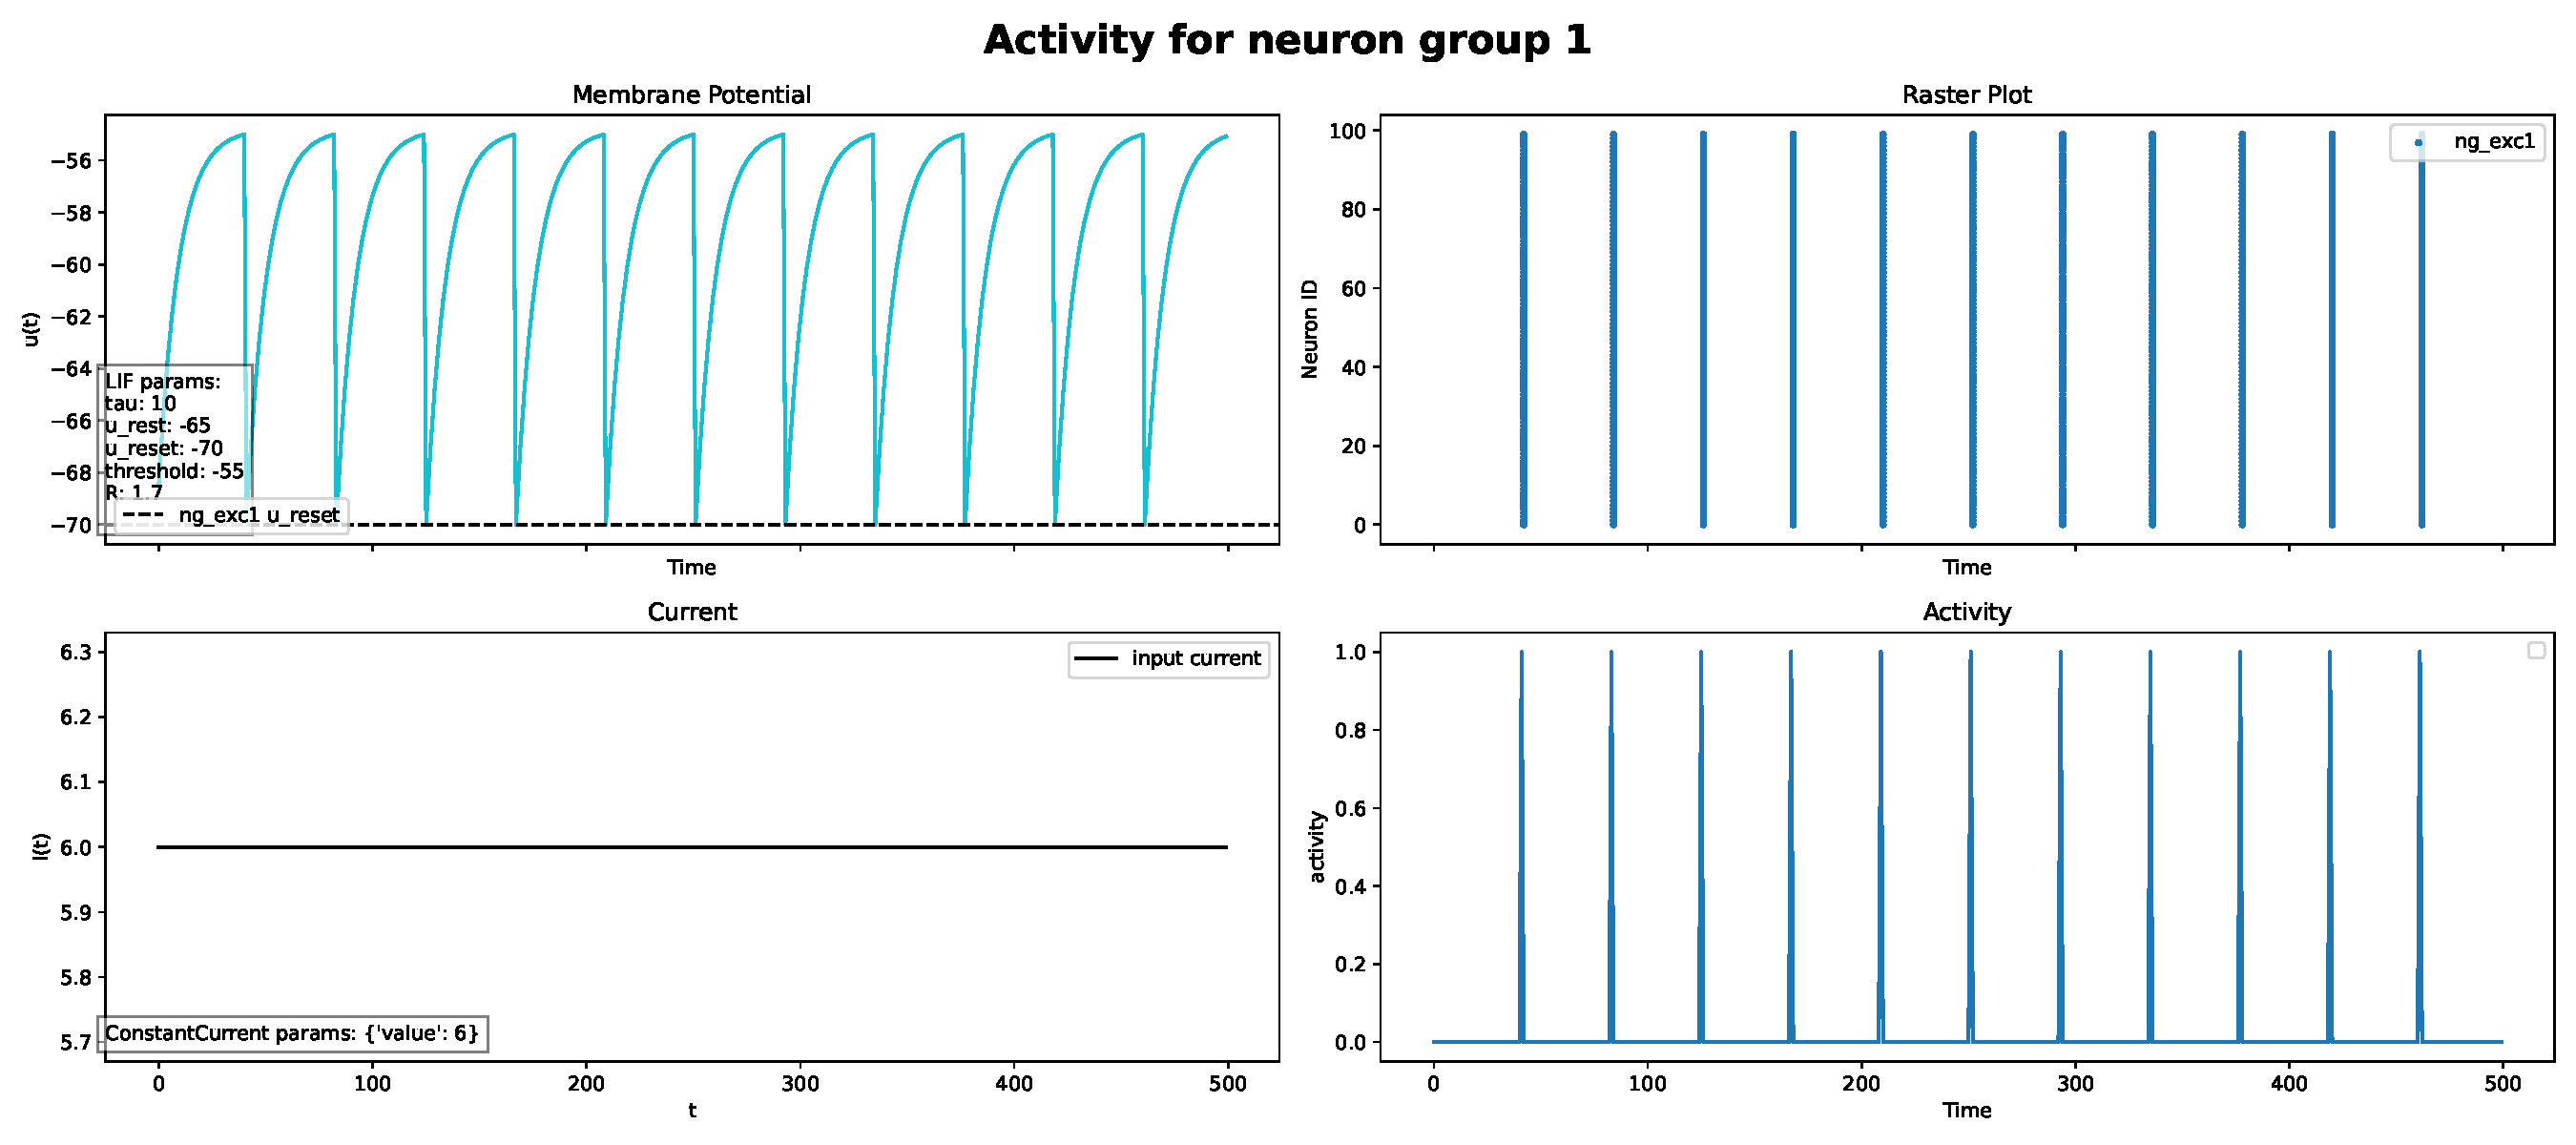
\includegraphics[width=0.9\textwidth]{plots/part1-Simple-ng-without-synapse.pdf} 
            \caption{جمعیت نورونی بدون سیناپس}
            \label{fig:part1-simple-ng}
        \end{figure}

        حال بیاید مقادیر اولیه نورون ها مانند اختلاف پتانسیل اولیه آن ها را تغییر دهیم تا رفتار آن ها را ببینیم. برای اینکار، اختلاف پتانسیل اولیه نورون ها را در حدود بازه ۶۷ با واریانس ۲ توزیع میکنیم. همانطور که در شکل
        \ref{fig:part1-simple-ng-u-init}
        نیز مشاهده می کنیم، نورون ها در ابتدا با یک اختلاف پتانسیل متفاوت شروع به فعالیت میکنند و از آنجا که جریان ورودی به آن ها نیز یکسان است، فواصل ضربه زدن خود را حفظ میکنند و با همان فواصل به ضربه زدن ادامه می دهند. در نتیجه فعالیت کلی جمعیت، به صورت دوره ای تکرار خواهد شد.
        \begin{figure}[!ht]
            \centering
            \includegraphics[width=0.9\textwidth]{plots/part1-Simple-ng-without-synapse-u\_init.pdf} 
            \caption{جمعیت نورونی بدون سیناپس: اختلاف پتانسیل اولیه متفاوت}
            \label{fig:part1-simple-ng-u-init}
        \end{figure}

        حال اگر به همین جمعیت یک جریان نویز دار اضافه کنیم چه اتفاقی می افتد؟ برای اینکار یک رفتار
        (\lr{Behavior})
        به نام 
        \texttt{NoiseCurrent}
        تعریف میکنیم که وظیفه آن اضافه کردن نویز به جریان نورون باشد. مقدار این نویز را یک جریان رندوم با میانگین ۰ و واریانس ۰.۱ قرار می دهیم. همانطور که در شکل 
        \ref{fig:part1-simple-ng-u-init-noise-curr}
        مشاهده میکنیم، به دلیل اضافه شدن نویز، الگوی فعالت نورون ها در بازه هایی که ضربه میزنند رفته رفته تغییر کرده و الگوی خود را از دست می دهند. هر چند اگر میزان این نویز خیلی زیاد باشد، می تواند برآیند جریان ورودی را زیاد کرده، به نحوی که رفتار نورون ها پس از مدتی مشابه شود.
        (شکل \ref{fig:part1-simple-ng-u-init-high-noise-curr})
        \begin{figure}[!ht]
            \centering
            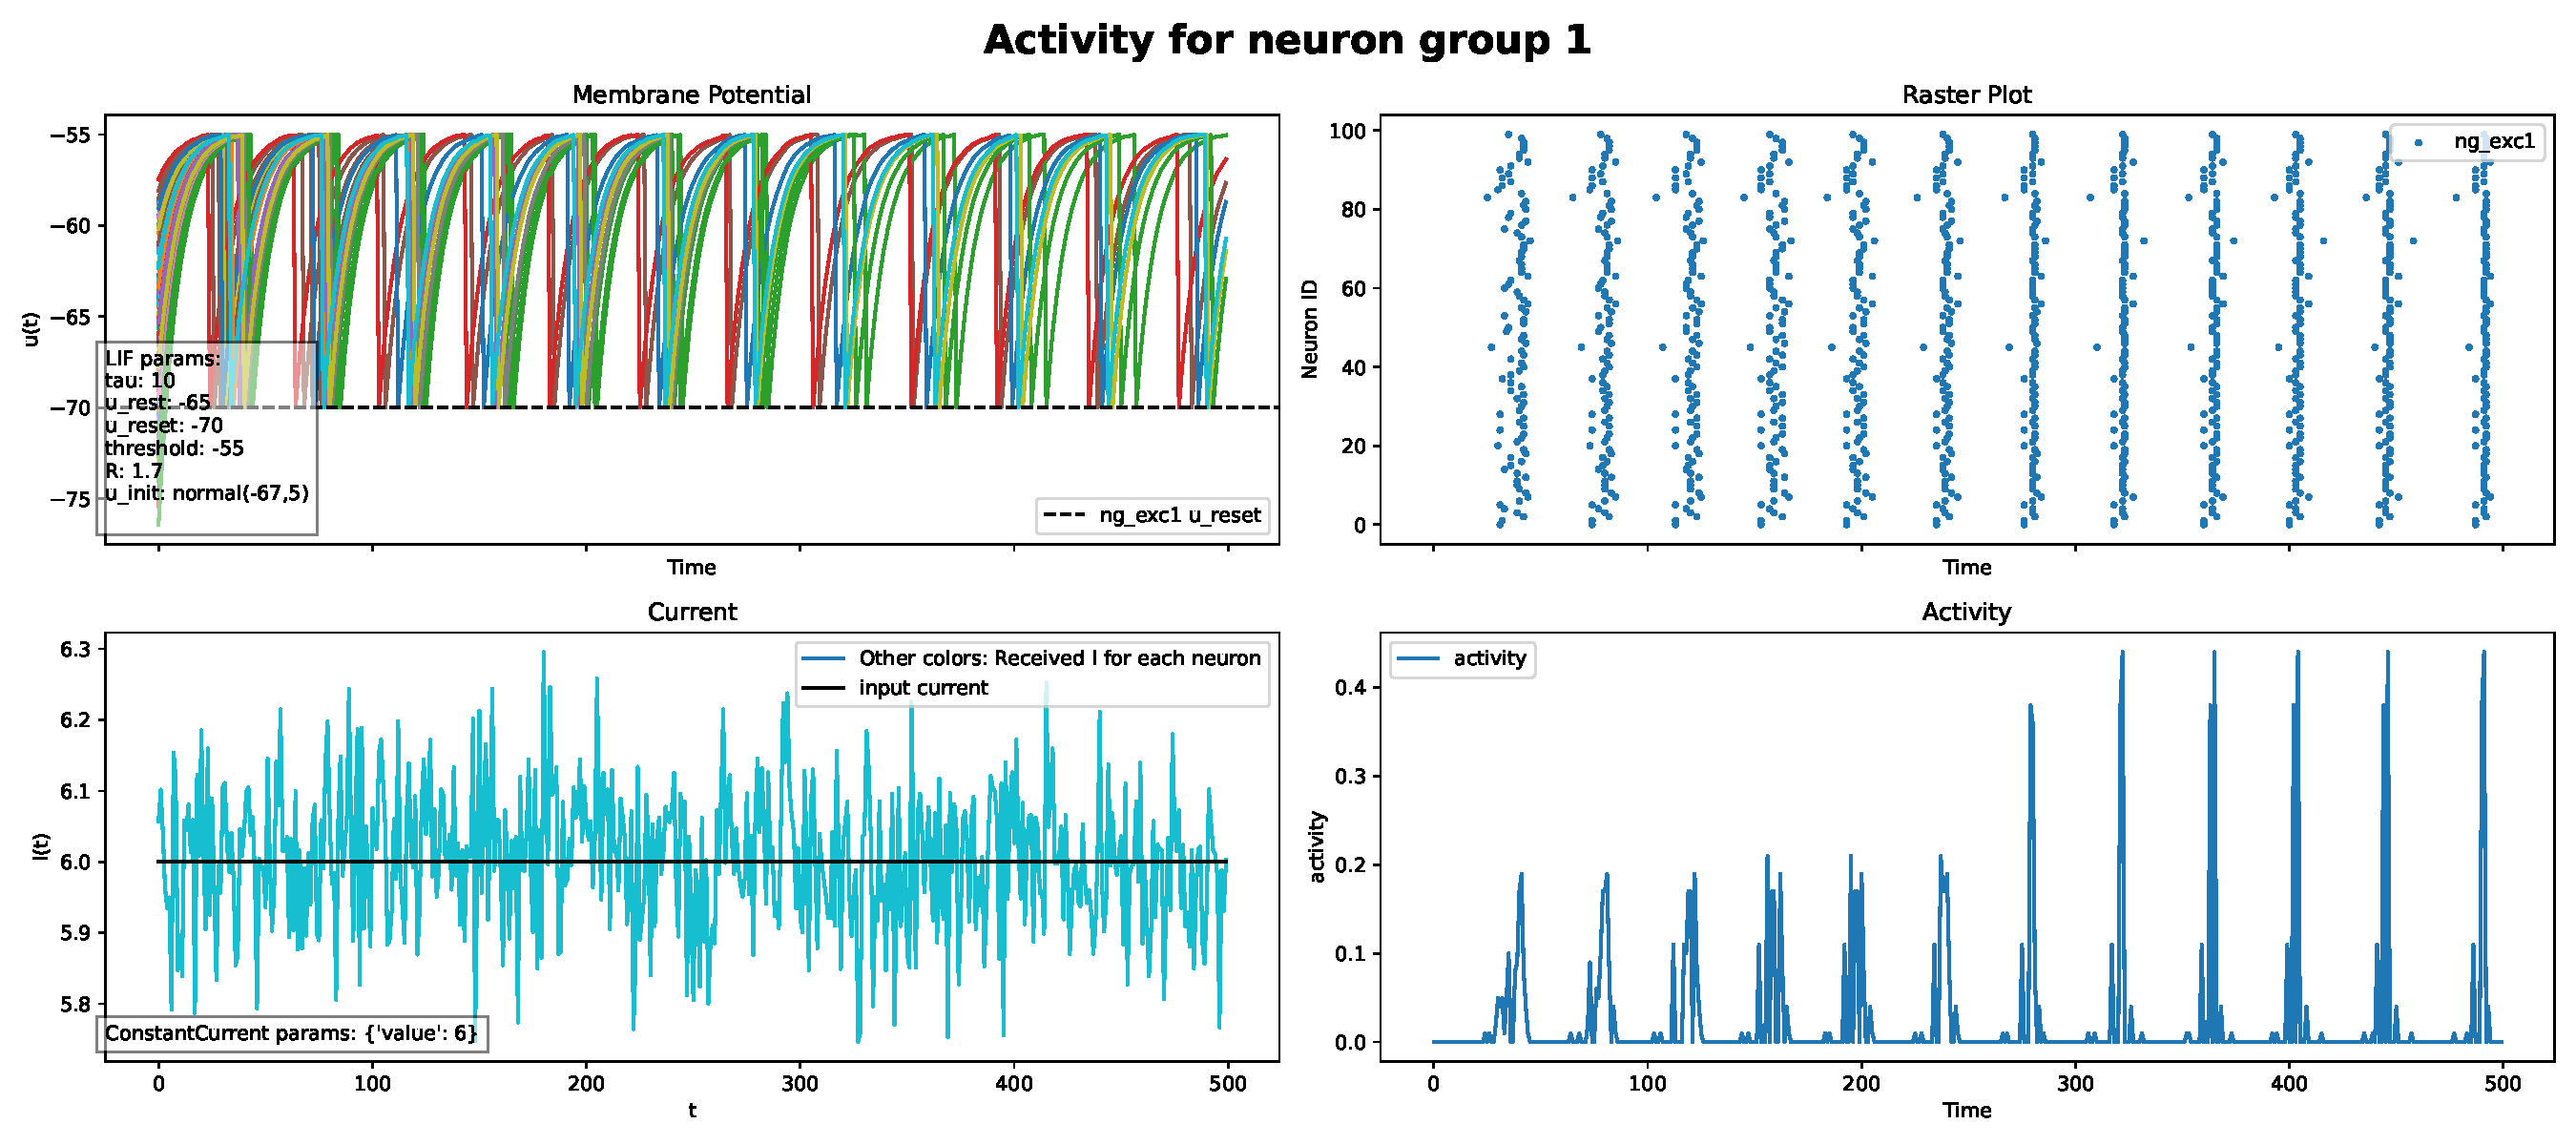
\includegraphics[width=0.9\textwidth]{plots/part1-Simple-ng-without-synapse-noise-curr.pdf} 
            \caption{جمعیت نورونی بدون سیناپس: اختلاف پتانسیل اولیه متفاوت و جریان نویزی}
            \label{fig:part1-simple-ng-u-init-noise-curr}
        \end{figure}
        \begin{figure}[!ht]
            \centering
            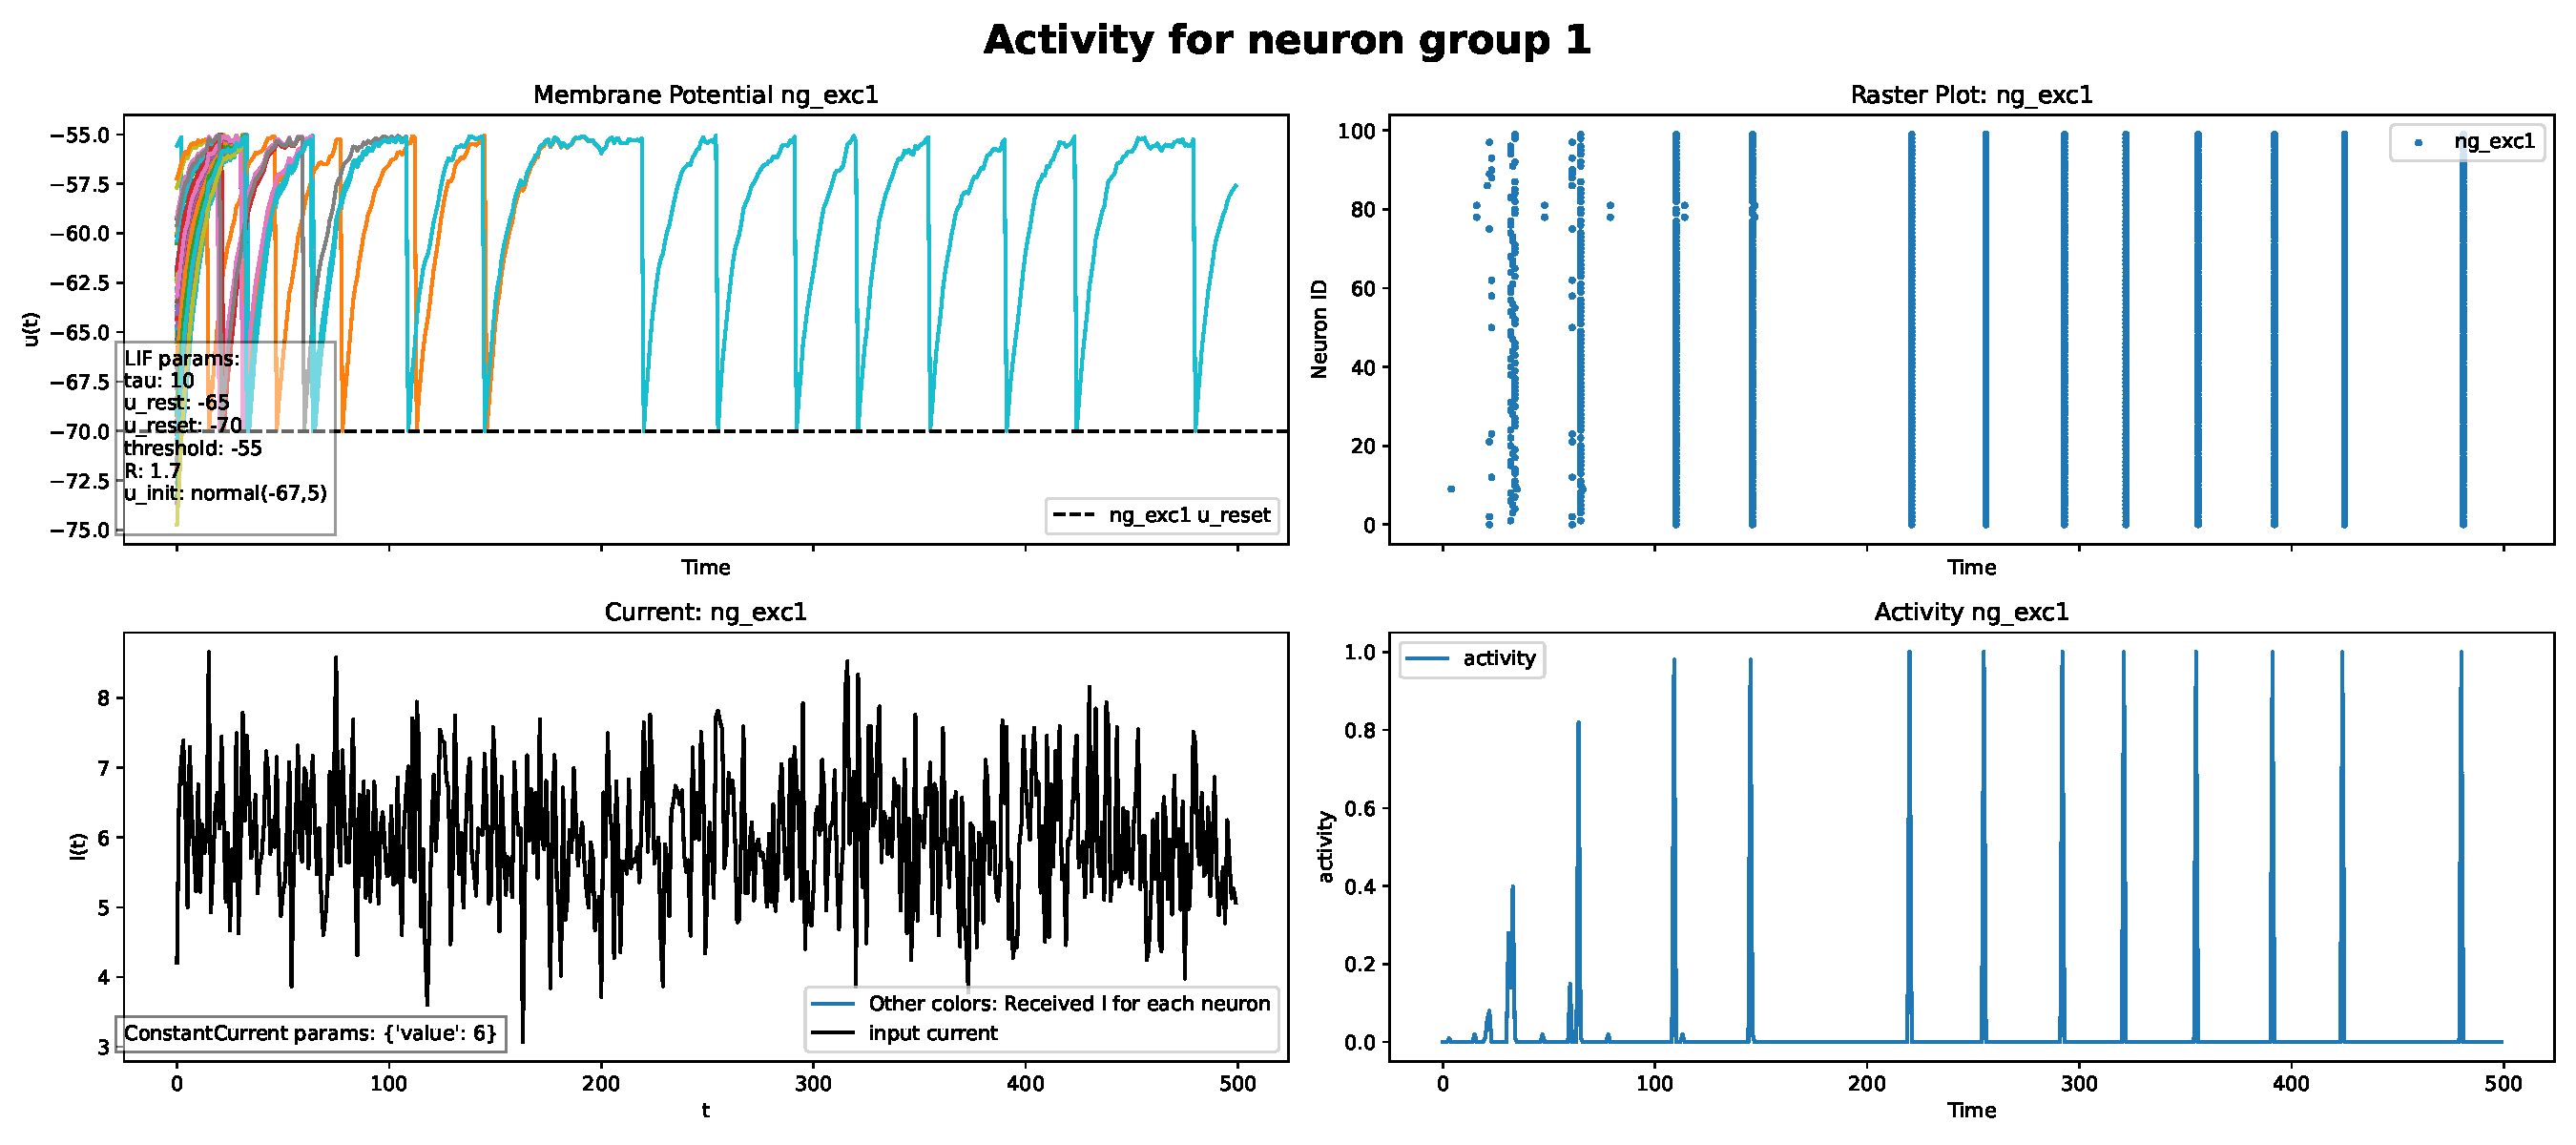
\includegraphics[width=0.9\textwidth]{plots/part1-Simple-ng-without-synapse-high-noise-curr.pdf} 
            \caption{جمعیت نورونی بدون سیناپس: اختلاف پتانسیل اولیه متفاوت و جریان نویزی زیاد}
            \label{fig:part1-simple-ng-u-init-high-noise-curr}
        \end{figure}

        حال فعالیت جمعیت نورونی را با جریان متفاوت برای هر نورون آزمایش میکنیم تا رفتار آن ها را بر این اساس نیز مشاهده کنیم. برای اینکار، جریان ورودی به جمعیت نورونی را با واریانس 
        $0.2$
        اضافه میکنیم. همانطور که در شکل 
        \ref{fig:part1-simple-ng-variance-curr}
        مشاهده میکنیم، تغییر دادن جریان ورودی به ازای هر نورون، زمان ضربه زدن هر نورون را از دیگری نسبت به حالت های قبل بیشتر متفاوت می کند و در نتیجه، پراکندگی زمان فعالیت نورون ها بیشتر می شود. همچنین اضافه کردن واریانس بیشتر میتواند پراکندگی را آنقدر افزایش دهد تا تشخیص یک الگو برای زمان ضربه زدن نورون ها بسیار سخت تر شود
        (شکل \ref{fig:part1-simple-ng-high-variance-curr})
        \begin{figure}[!ht]
            \centering
            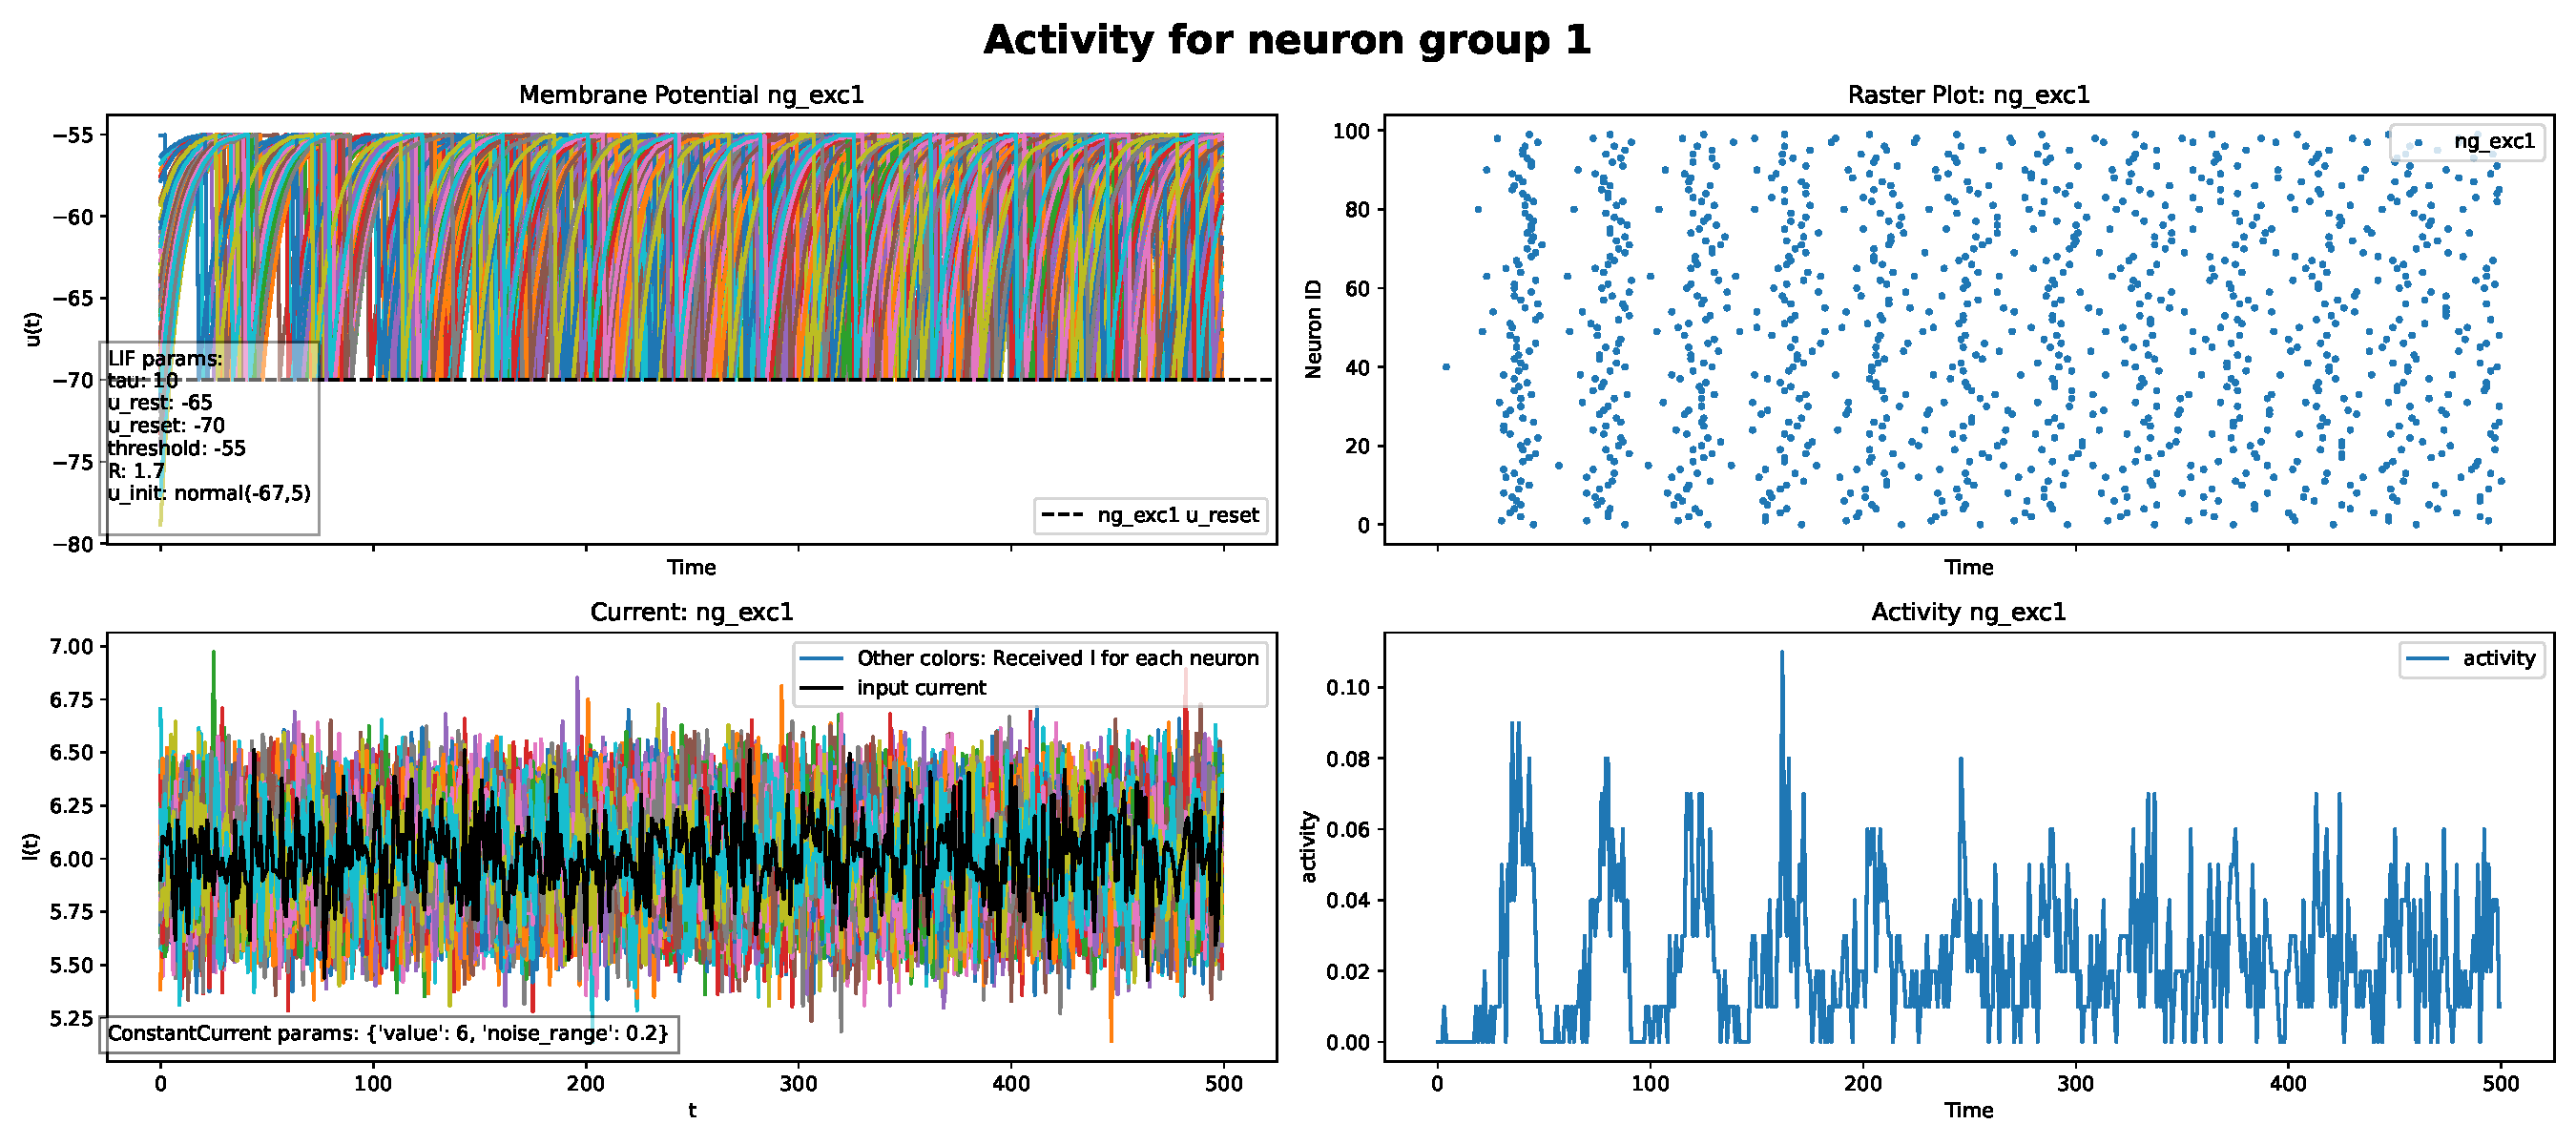
\includegraphics[width=0.9\textwidth]{plots/part1-Simple-ng-without-synapse-variance-curr.pdf} 
            \caption{جمعیت نورونی بدون سیناپس: جریان ورودی متفاوت}
            \label{fig:part1-simple-ng-variance-curr}
        \end{figure}
        \begin{figure}[!ht]
            \centering
            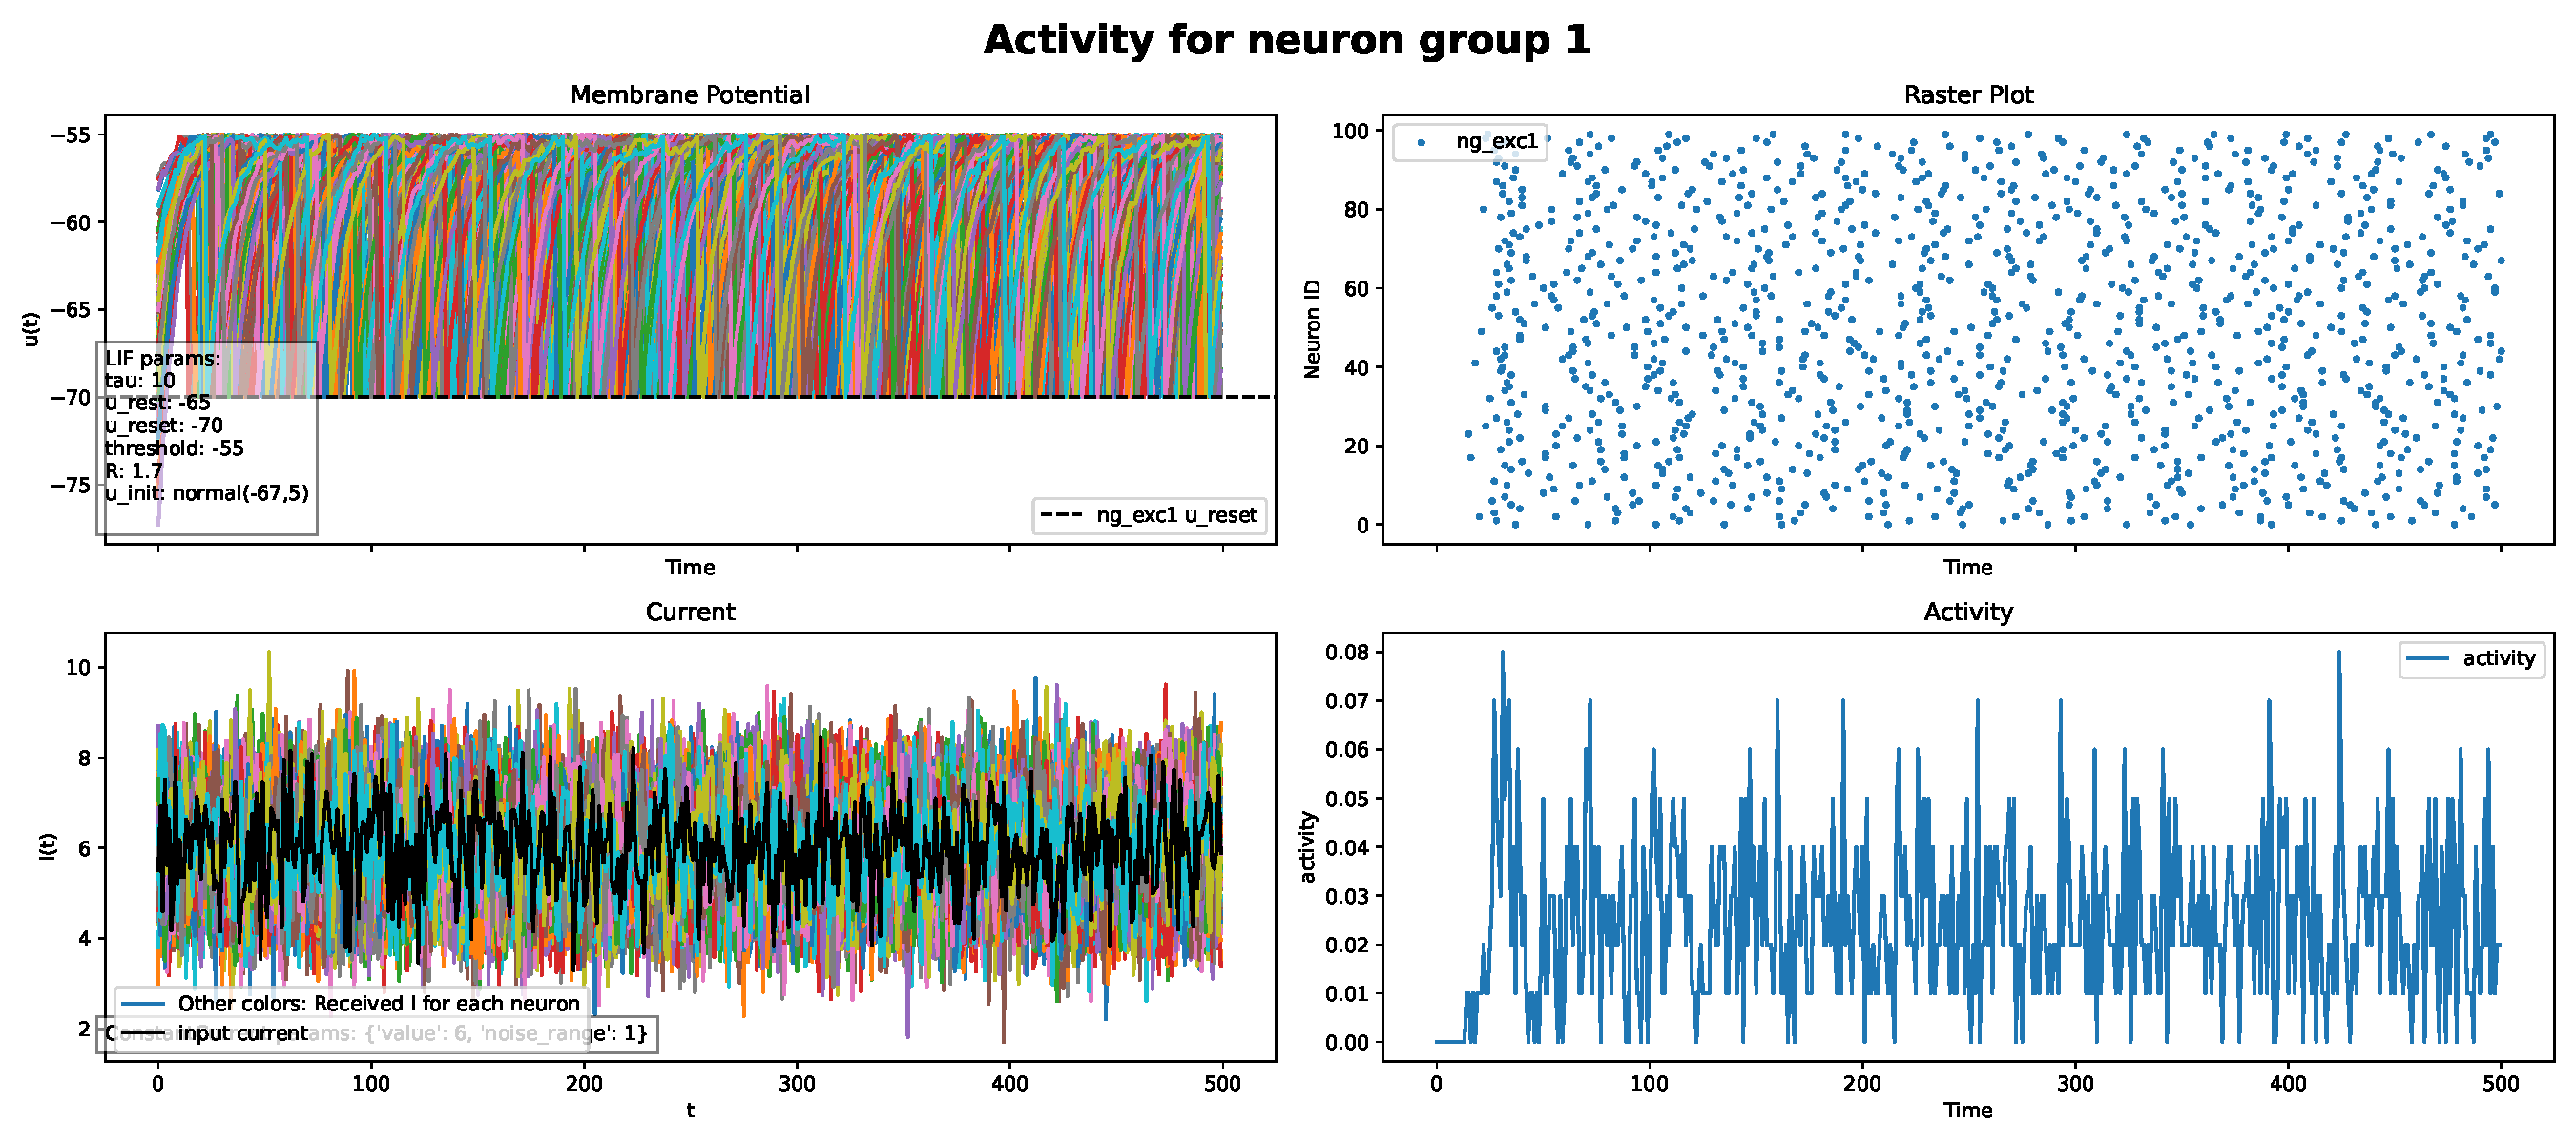
\includegraphics[width=0.9\textwidth]{plots/part1-Simple-ng-without-synapse-high-variance-curr.pdf} 
            \caption{جمعیت نورونی بدون سیناپس: جریان ورودی با تفاوت زیاد}
            \label{fig:part1-simple-ng-high-variance-curr}
        \end{figure}

        \subsubsection*{جمعیت نورونی به همراه سیناپس}
        حال که تاثیر انواع متفاوت جریان را بر یک جمعیت نورونی بررسی کردیم، به سراغ اضافه کردن سیناپس به آن میرویم. برای سادگی، سیناپس را با الگوی ارتباط کامل
        \footnote{\lr{full connectivity}}
        بررسی میکنیم و بررسی الگو های دیگر را به بخش دوم پروژه واگذار میکنیم. در ابتدا نیز وزن های سیناپسی را کامل یکسان با
        $j_0=5$ و $\sigma=0$
        در نظر میگیریم و سپس به آن واریانس اضافه میکنیم. همانطور که در شکل
        \ref{fig:part1-simple-ng-with-synapse}
        ملاحظه میکنیم، در یک جمعیت نورونی به همراه سیناپس داخلی، که نورون ها نیز در زمان اولیه اختلاف پتانسیل یکسانی دارند، رفتار جمعیت همانند هنگامی است که سیناپس وجود نداشته باشد. این به این دلیل است که در این حالت، قبل از اولین ضربه سیناپس تاثیری ندارد و رفتار نورون  همانند جمعیت بدون سیناپس با جریان ورودی ثابت است. از این رو اختلاف پتانسیل نورون ها به طور همزمان افزایش می یابد تا هنگامی که به  آستانه رسیده و نورون ها همزمان ضربه می زنند. در این لحظه، بلافاصله جریان سیناپسی نیز به جریان دریافتی نورون اضافه می شود و از آنجا که سیناپس ارتباط کامل است، زمان ضربه زدن نورون ها تغییری پیدا نمی کند.
        \begin{figure}[!ht]
            \centering
            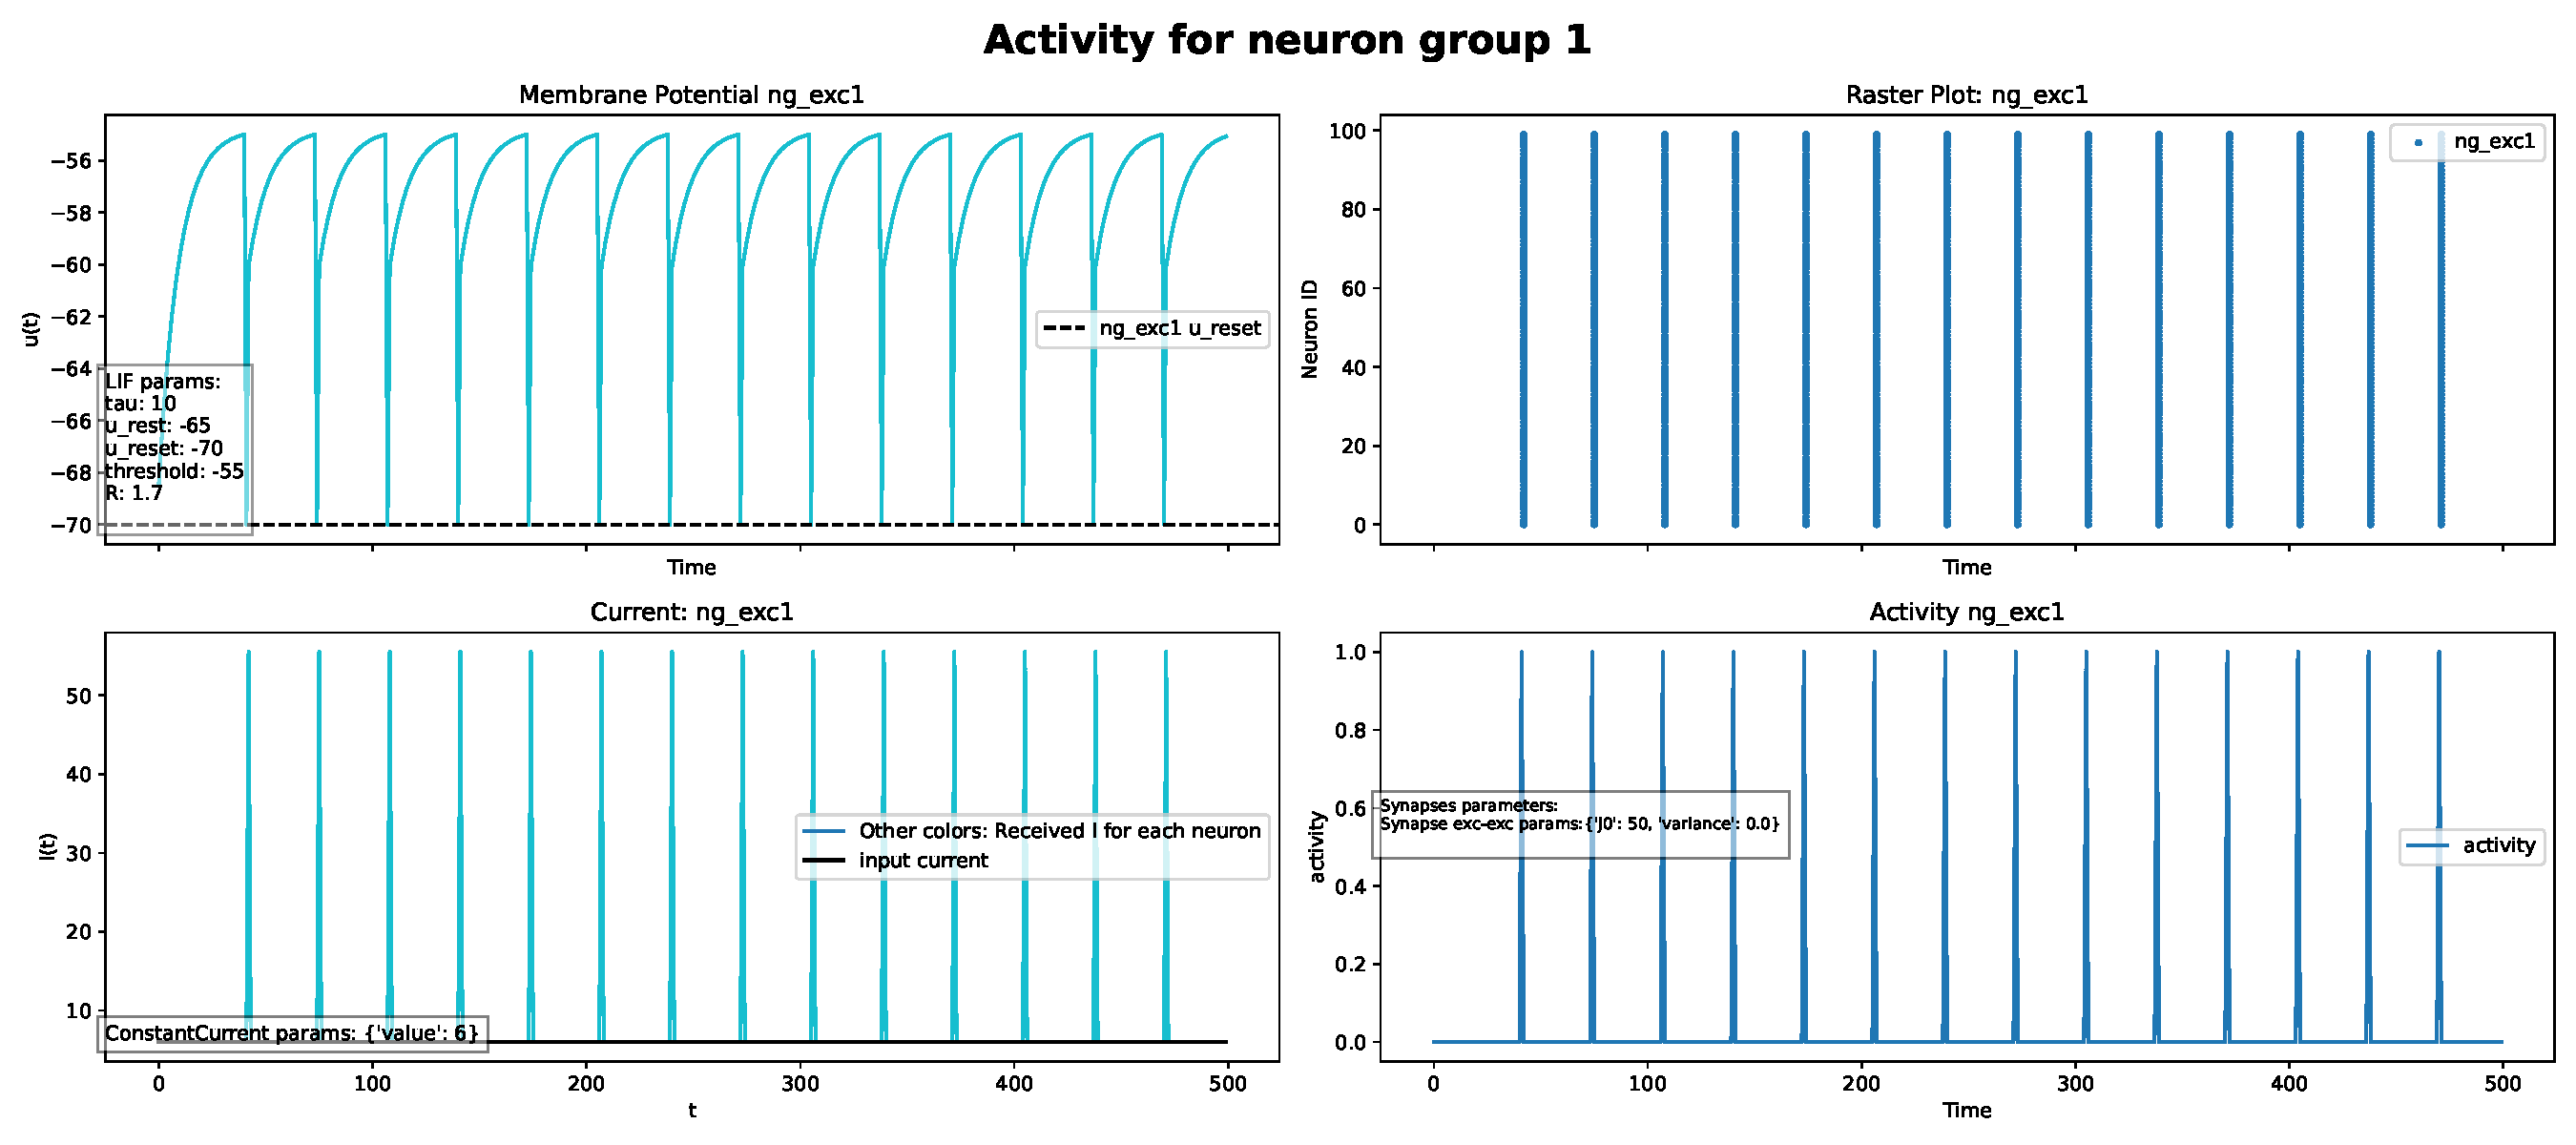
\includegraphics[width=0.9\textwidth]{plots/part1-Simple-ng-with-synapse.pdf} 
            \caption{جمعیت نورونی با سیناپس: جریان ثابت}
            \label{fig:part1-simple-ng-with-synapse}
        \end{figure}

        حال اگر اختلاف پتانسیل اولیه نورون ها را متفاوت مقدار دهی کنیم، مطابق شکل
        \ref{fig:part1-simple-ng-with-synapse-u-init}
        میبینیم که زمان ضربه زدن نورون ها متفاوت می شود.هر چند پس از مدتی، به دلیل اضافه شدن جریان سیناپسی به جریان ورودی نورون و درنتیجه افزایش یافتن جریان دریافتی نورون، این اختلاف زمانی ضربه ها نیز کمتر می شود. افزایش مقدار 
        $j_0$ 
        به ۱۰ نیز زمان این همگرایی را سریع تر می کند.
        (شکل \ref{fig:part1-simple-ng-with-synapse-u-init-high-j})
        \begin{figure}[!ht]
            \centering
            \includegraphics[width=0.9\textwidth]{plots/part1-Simple-ng-with-synapse-u\_init.pdf} 
            \caption{جمعیت نورونی با سیناپس: اختلاف پتانسیل اولیه متفاوت}
            \label{fig:part1-simple-ng-with-synapse-u-init}
        \end{figure}
        \begin{figure}[!ht]
            \centering
            \includegraphics[width=0.9\textwidth]{plots/part1-Simple-ng-with-synapse-u\_init-high\_j.pdf} 
            \caption{جمعیت نورونی با سیناپس: اختلاف پتانسیل اولیه متفاوت و وزن های بیشتر}
            \label{fig:part1-simple-ng-with-synapse-u-init-high-j}
        \end{figure}

        حال واریانس وزن های سیناپسی را از ۰ بیشتر میکنیم، تا تاثیر این پارامتر را بر روی رفتار جمعیت ملاحظه کنیم. انتظار داریم که افزودن پراکندگی به وزن ها باعث پراکندگی زمان ضربه زدن نورون ها نیز بشود. شکل 
        \ref{fig:part1-simple-ng-with-synapse-u_init-variance}
        این موضوع را تایید میکند و ملاظحه می شود که فعالیت نورون ها مانند شکل قبل همگرا نشده و بالا و پایین می شود
        (در نهایت بین مقادیر ۰.۶ و ۰.۸ نوسان می کند.)
        \begin{figure}[!ht]
            \centering
            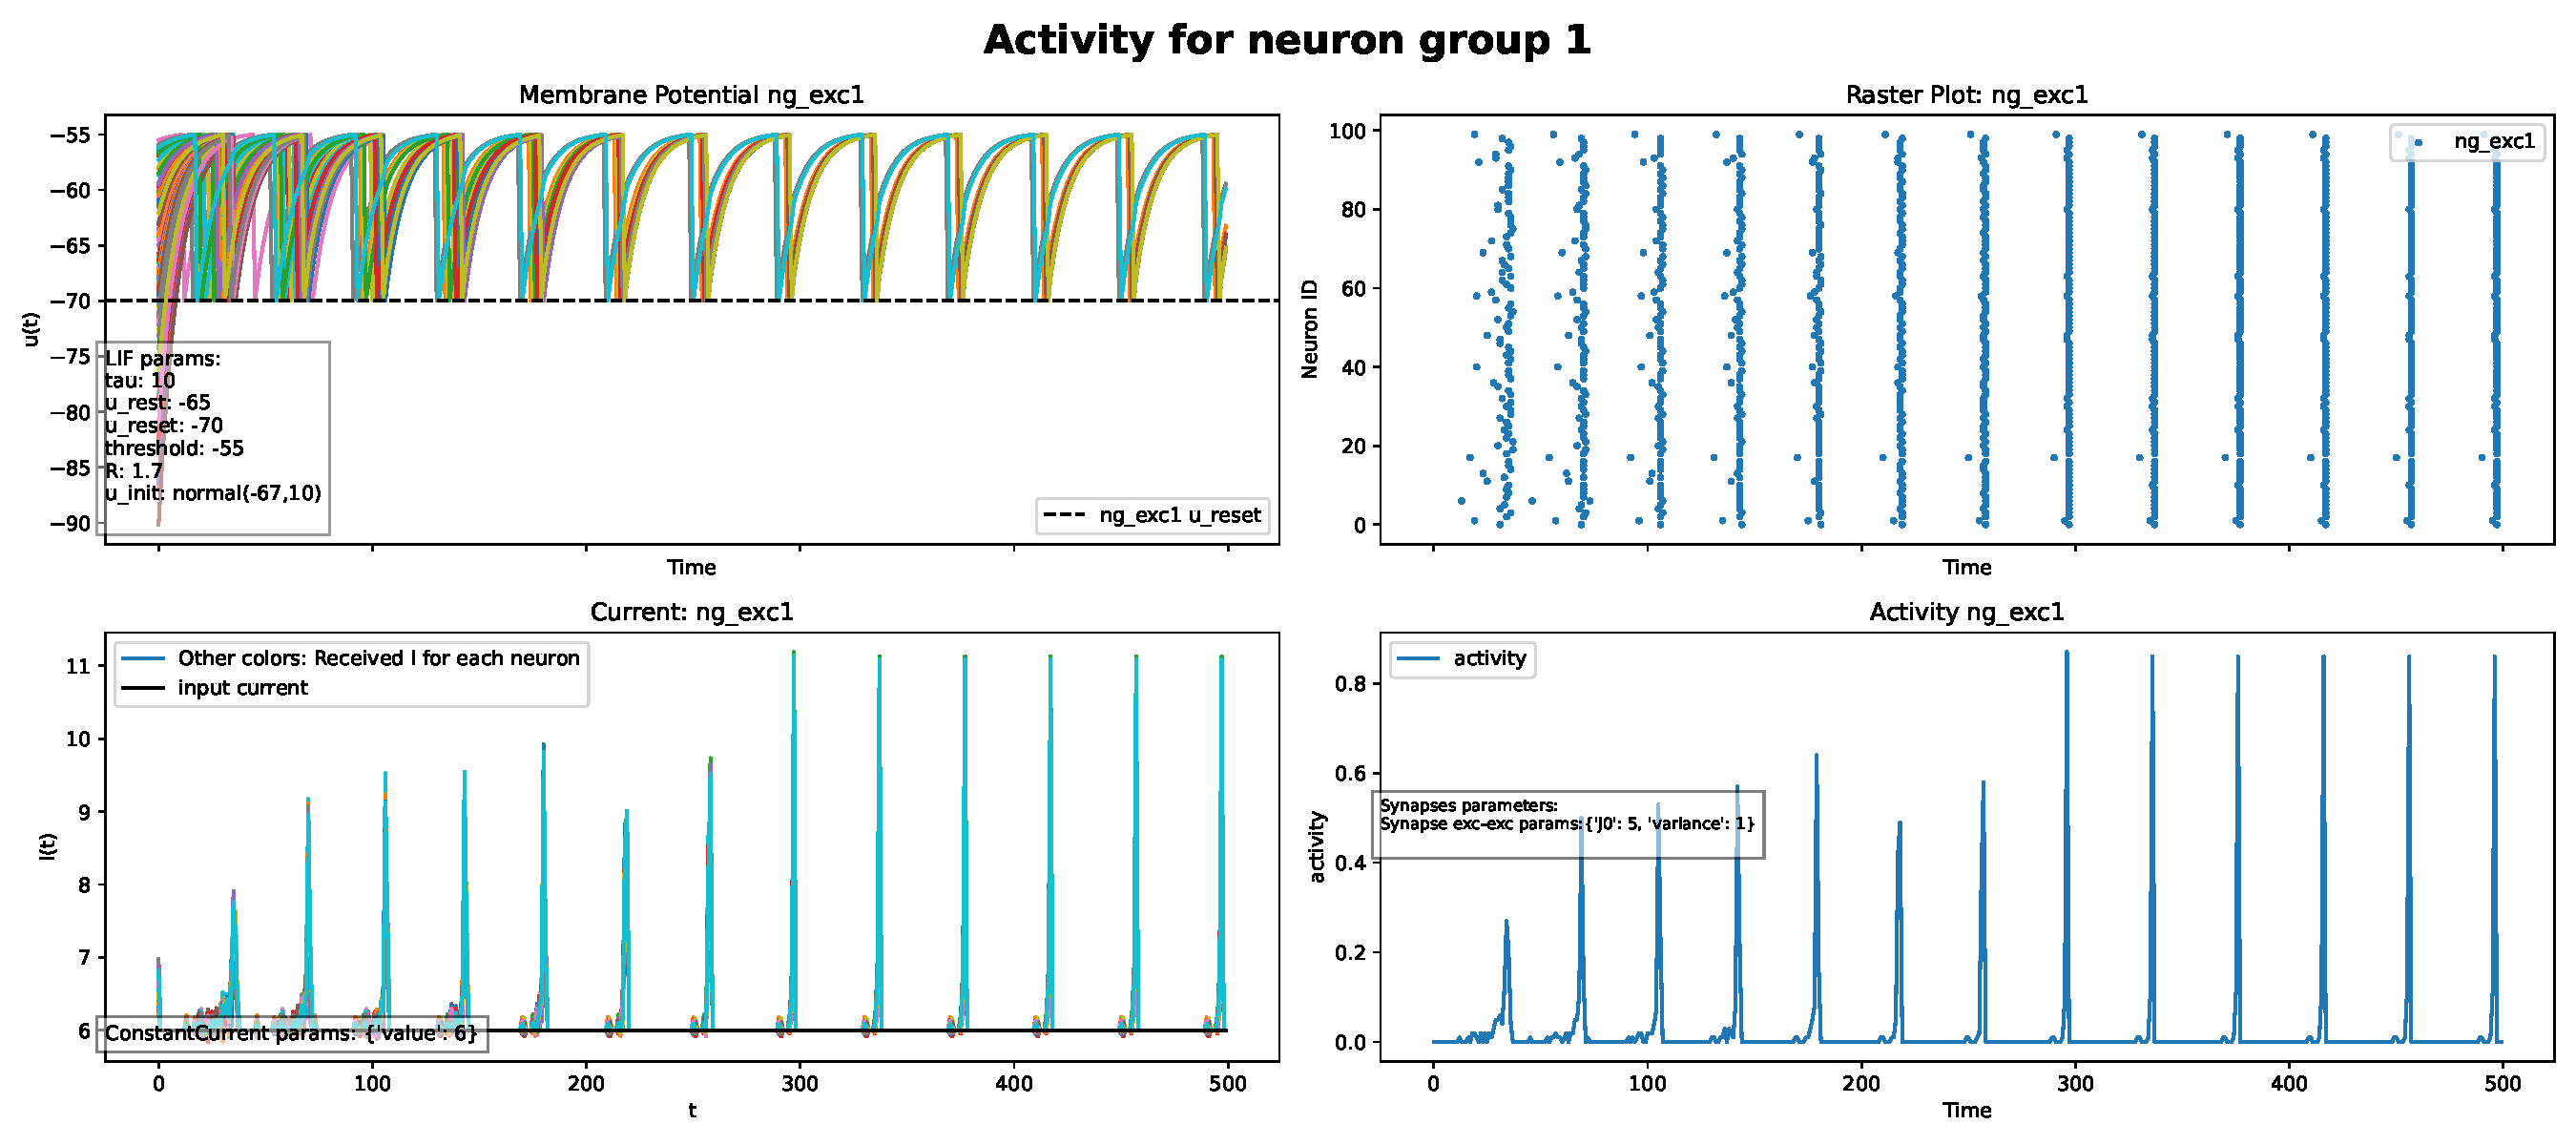
\includegraphics[width=0.9\textwidth]{plots/part1-Simple-ng-with-synapse-u_init-variance.pdf} 
            \caption{جمعیت نورونی با سیناپس: اختلاف پتانسیل اولیه متفاوت و وزن با واریانس بیشتر}
            \label{fig:part1-simple-ng-with-synapse-u_init-variance}
        \end{figure}
        بعد از بررسی پارامتر های سیناپس، نوبت به بررسی تاثیر جریان بر روی سیناپس می رسد. مطابق زیربخش قبل، در ابتدا رفتار جمعیت را با جریان نویزی یکسان برای همه نورون ها بررسی میکنیم. همانطور که در شکل
        \ref{fig:part1-simple-ng-with-synapse-noise-curr}
        مشاهده می شود، در ابتدا، زمان ضربه زدن نورون ها با یکدیگر متفاوت است و پس از مدتی این تفاوت کاهش یافته و همگرا می شود به طور که در نمودار فعالیت مشاهده می کنیم که ابتدا فعالیت نورونی حدود ۰ بوده و در نهایت به ۱ می رسد.
        \begin{figure}[!ht]
            \centering
            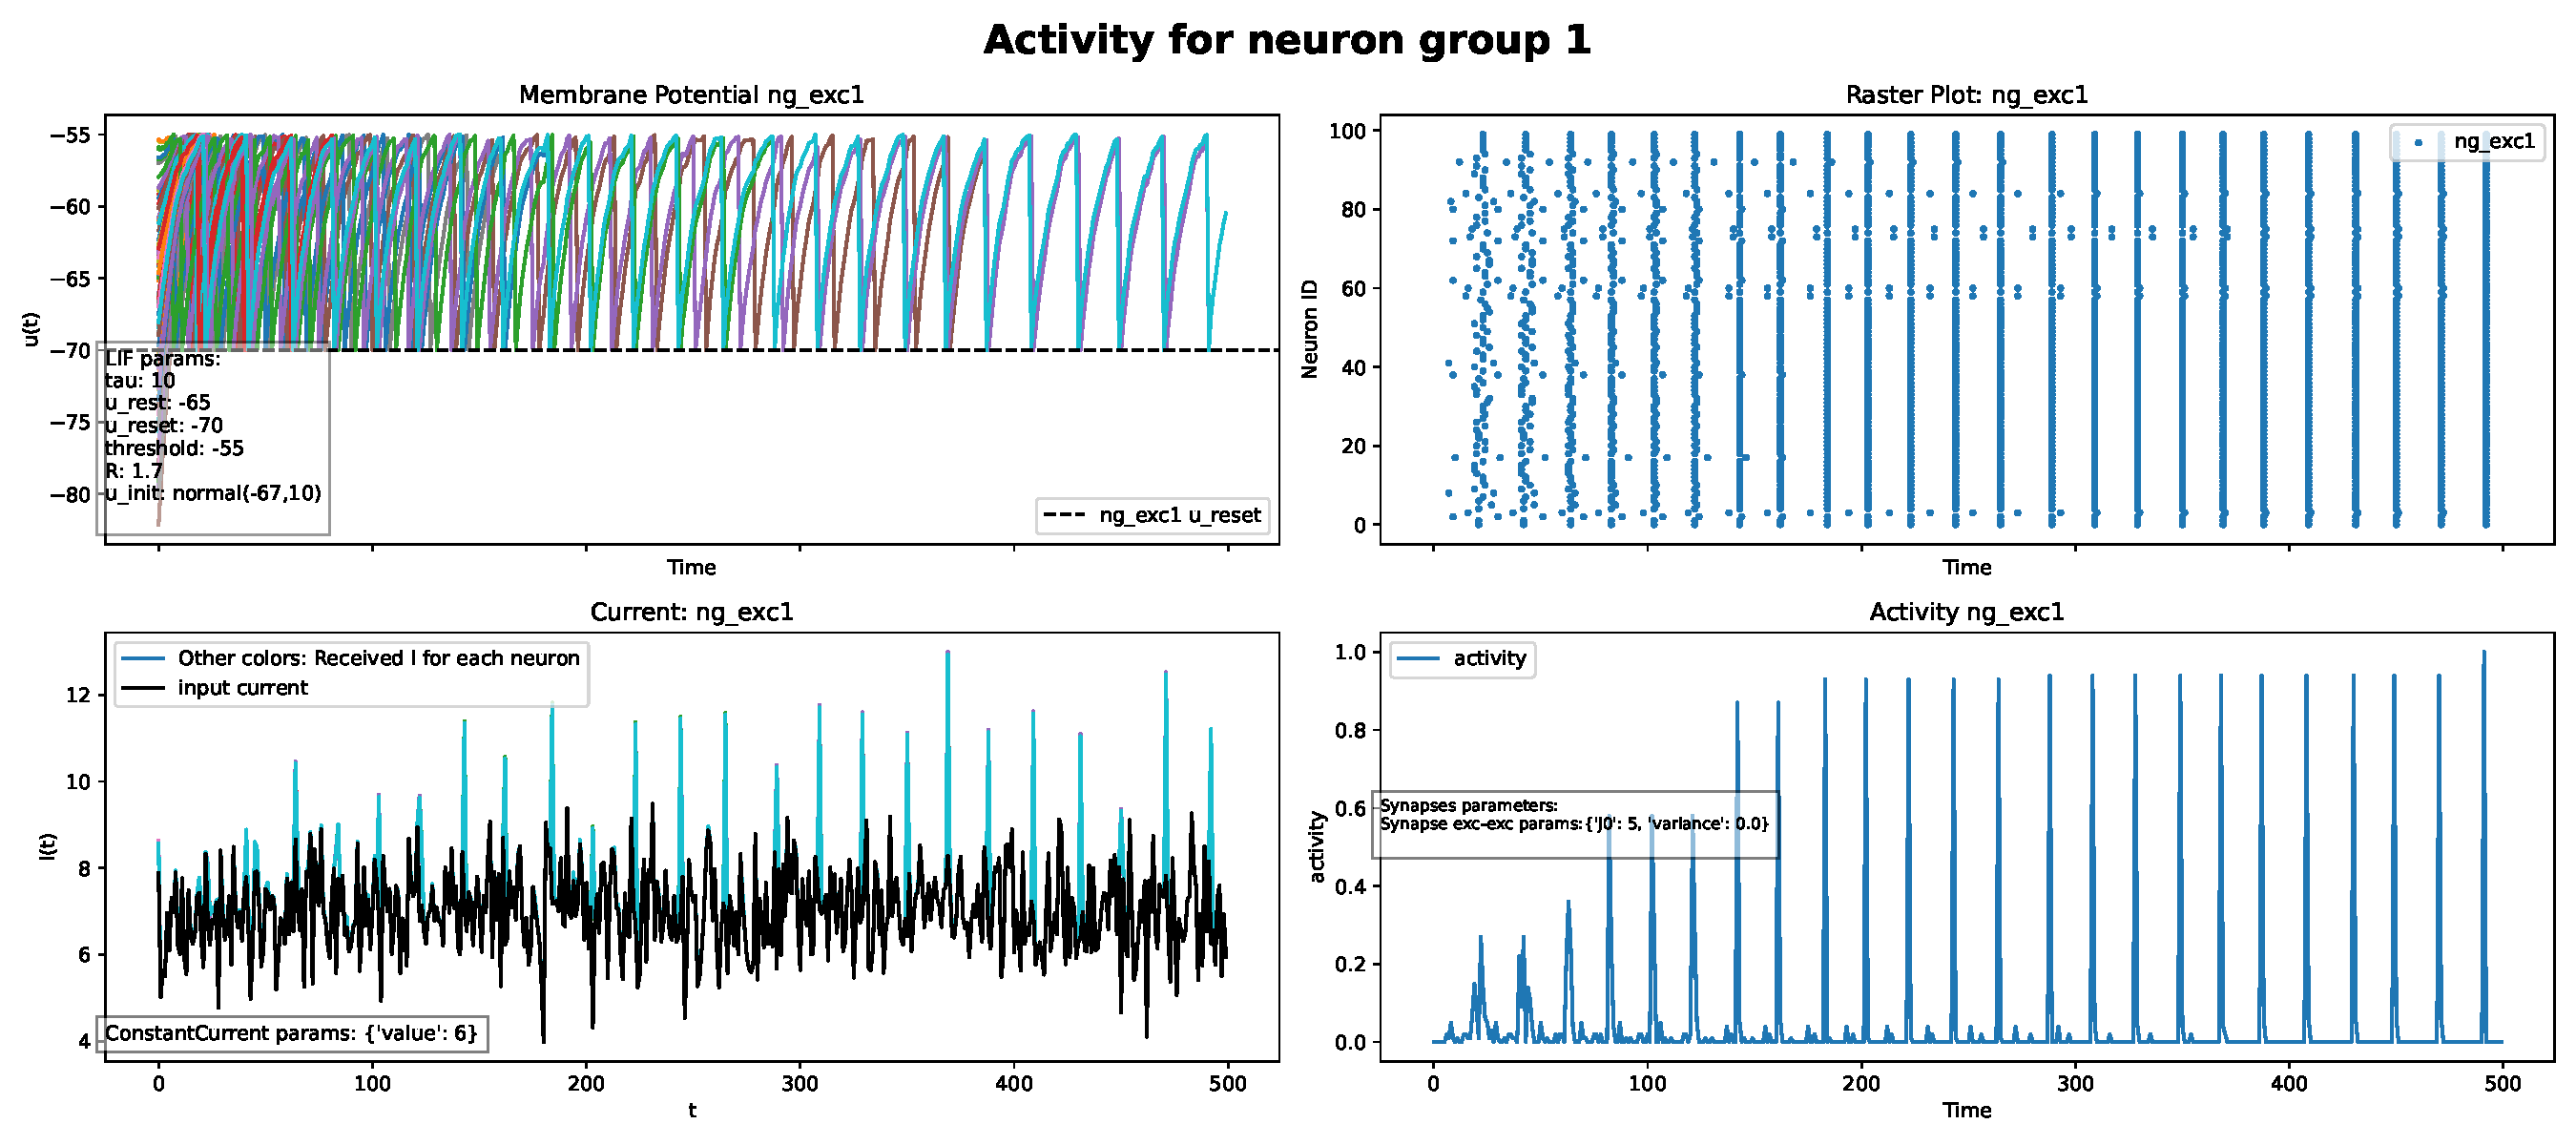
\includegraphics[width=0.9\textwidth]{plots/part1-Simple-ng-with-synapse-noise-curr.pdf} 
            \caption{جمعیت نورونی با سیناپس: اختلاف پتانسیل اولیه متفاوت و جریان نویز دار}
            \label{fig:part1-simple-ng-with-synapse-noise-curr}
        \end{figure}

        اکنون نوبت به آزمایش رفتار جمعیت نسبت به جریان متفاوت می رسد. در این آزمایش، رفتار جمعیت را با جریان نویزی برای نورون های مختلف با دامنه نوسان 0.6 بررسی میکنیم. همانطور که در شکل
        \ref{fig:part1-simple-ng-with-synapse-diff-curr}
        مشاهده می شود، داشتن جریان های متفاوت سبب می شود که زمان ضربه زدن نورون ها پارکندگی بیشتر نسبت به قبل داشته باشد ولی برخلاف جمعیت بدون سیناپس که این پراکندگی کاهش نمی یافت، در جمعیت دارای سیناپس مشاهده میکنیم که پس از مدتی، پراکندگی زمان ضربه زدن نورون ها کاهش یافته و در نتیجه فعالیت جمعیت بیشتر میشود.
        \begin{figure}[!ht]
            \centering
            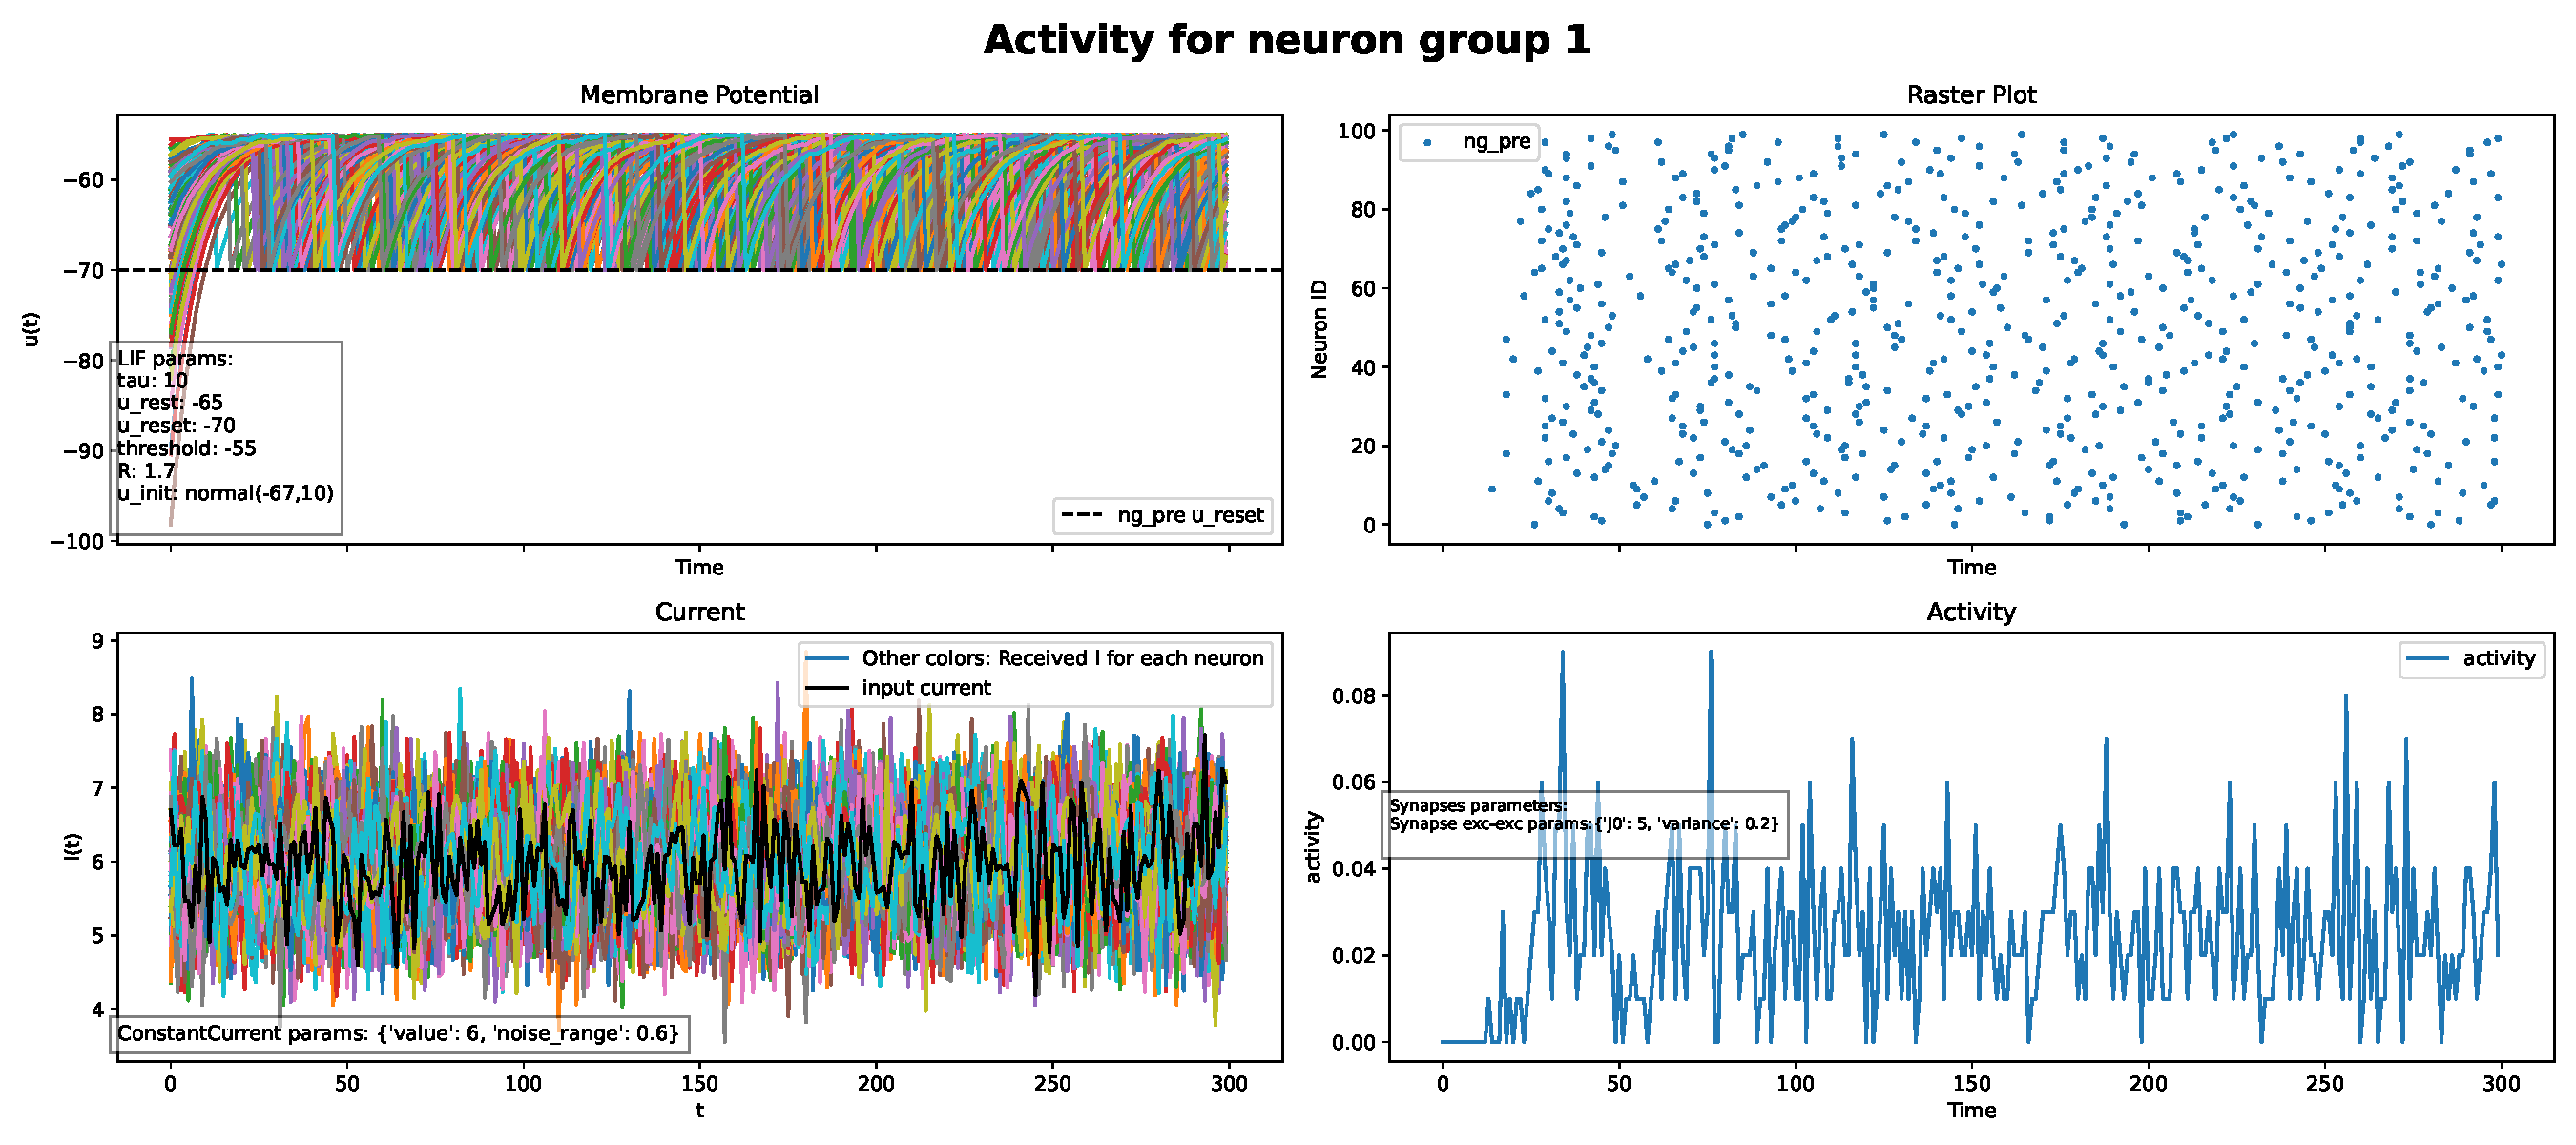
\includegraphics[width=0.9\textwidth]{plots/part1-Simple-ng-with-synapse-diff-curr.pdf} 
            \caption{جمعیت نورونی با سیناپس: اختلاف پتانسیل اولیه متفاوت و جریان نویزی غیریکسان}
            \label{fig:part1-simple-ng-with-synapse-diff-curr}
        \end{figure}

    \subsection{بررسی رفتار دو جمعیت نورونی}
        پس از بررسی رفتار یک جمعیت نورونی در حضور سیناپس، اکنون به سراغ بررسی رفتار دو جمعیت نورونی که از یکی به دیگری سیناپس وجود دارد می رویم. در این بخش تنها حالتی را در نظر میگیریم که یک جمعیت، نورون های پیش سیناپسی را تشکیل داده و جمعیت دیگر نورون های پس سیناپسی. بررسی حالت هایی با سیناپس های بیشتر را به بخش های بعدی واگذار میکنیم.

        برای اینکار، ابتدا دو جمعیت نورونی تحریکی کاملا مشابه تشکیل میدهیم که فقط از جمعیت اول به جمعیت دوم سیناپس داریم. همچنین جریان ورودی هر دو جمعیت را نیز یکسان و ثابت میگیریم. حال اگر شبیه سازی را انجام دهیم، در شکل
        \ref{fig:part1-two-ng-with-synapse}
        ملاحظه میکنیم که زمان ضربه زدن نورون های هر دو جمعیت کاملا یکسان است که این موضوع مربوط به کاملا یکسان بودن این دو جمعیت است. همچنین به دلیل اینکه در پیاده سازی سیناپس، طبق گفته حل تمرین مربوطه، نیازی نیست تا تاثیر سیناپس تا لحظات بعد نیز باقی بماند، عملا افزایش لحظه ای جریان ورودی به نورون های پس سیناپسی بی تاثیر می شود. اما اگر بتوان تاثیر جریان های موجود در سیناپس را حفظ نمود، ضربه های نورون پیش سیناپسی نیز روی نورون های پس سیناپسی تاثیر گذار خواهد بود
        (شکل \ref{fig:part1-two-ng-with-synapse-decay})
        \begin{figure}[!ht]
            \centering
            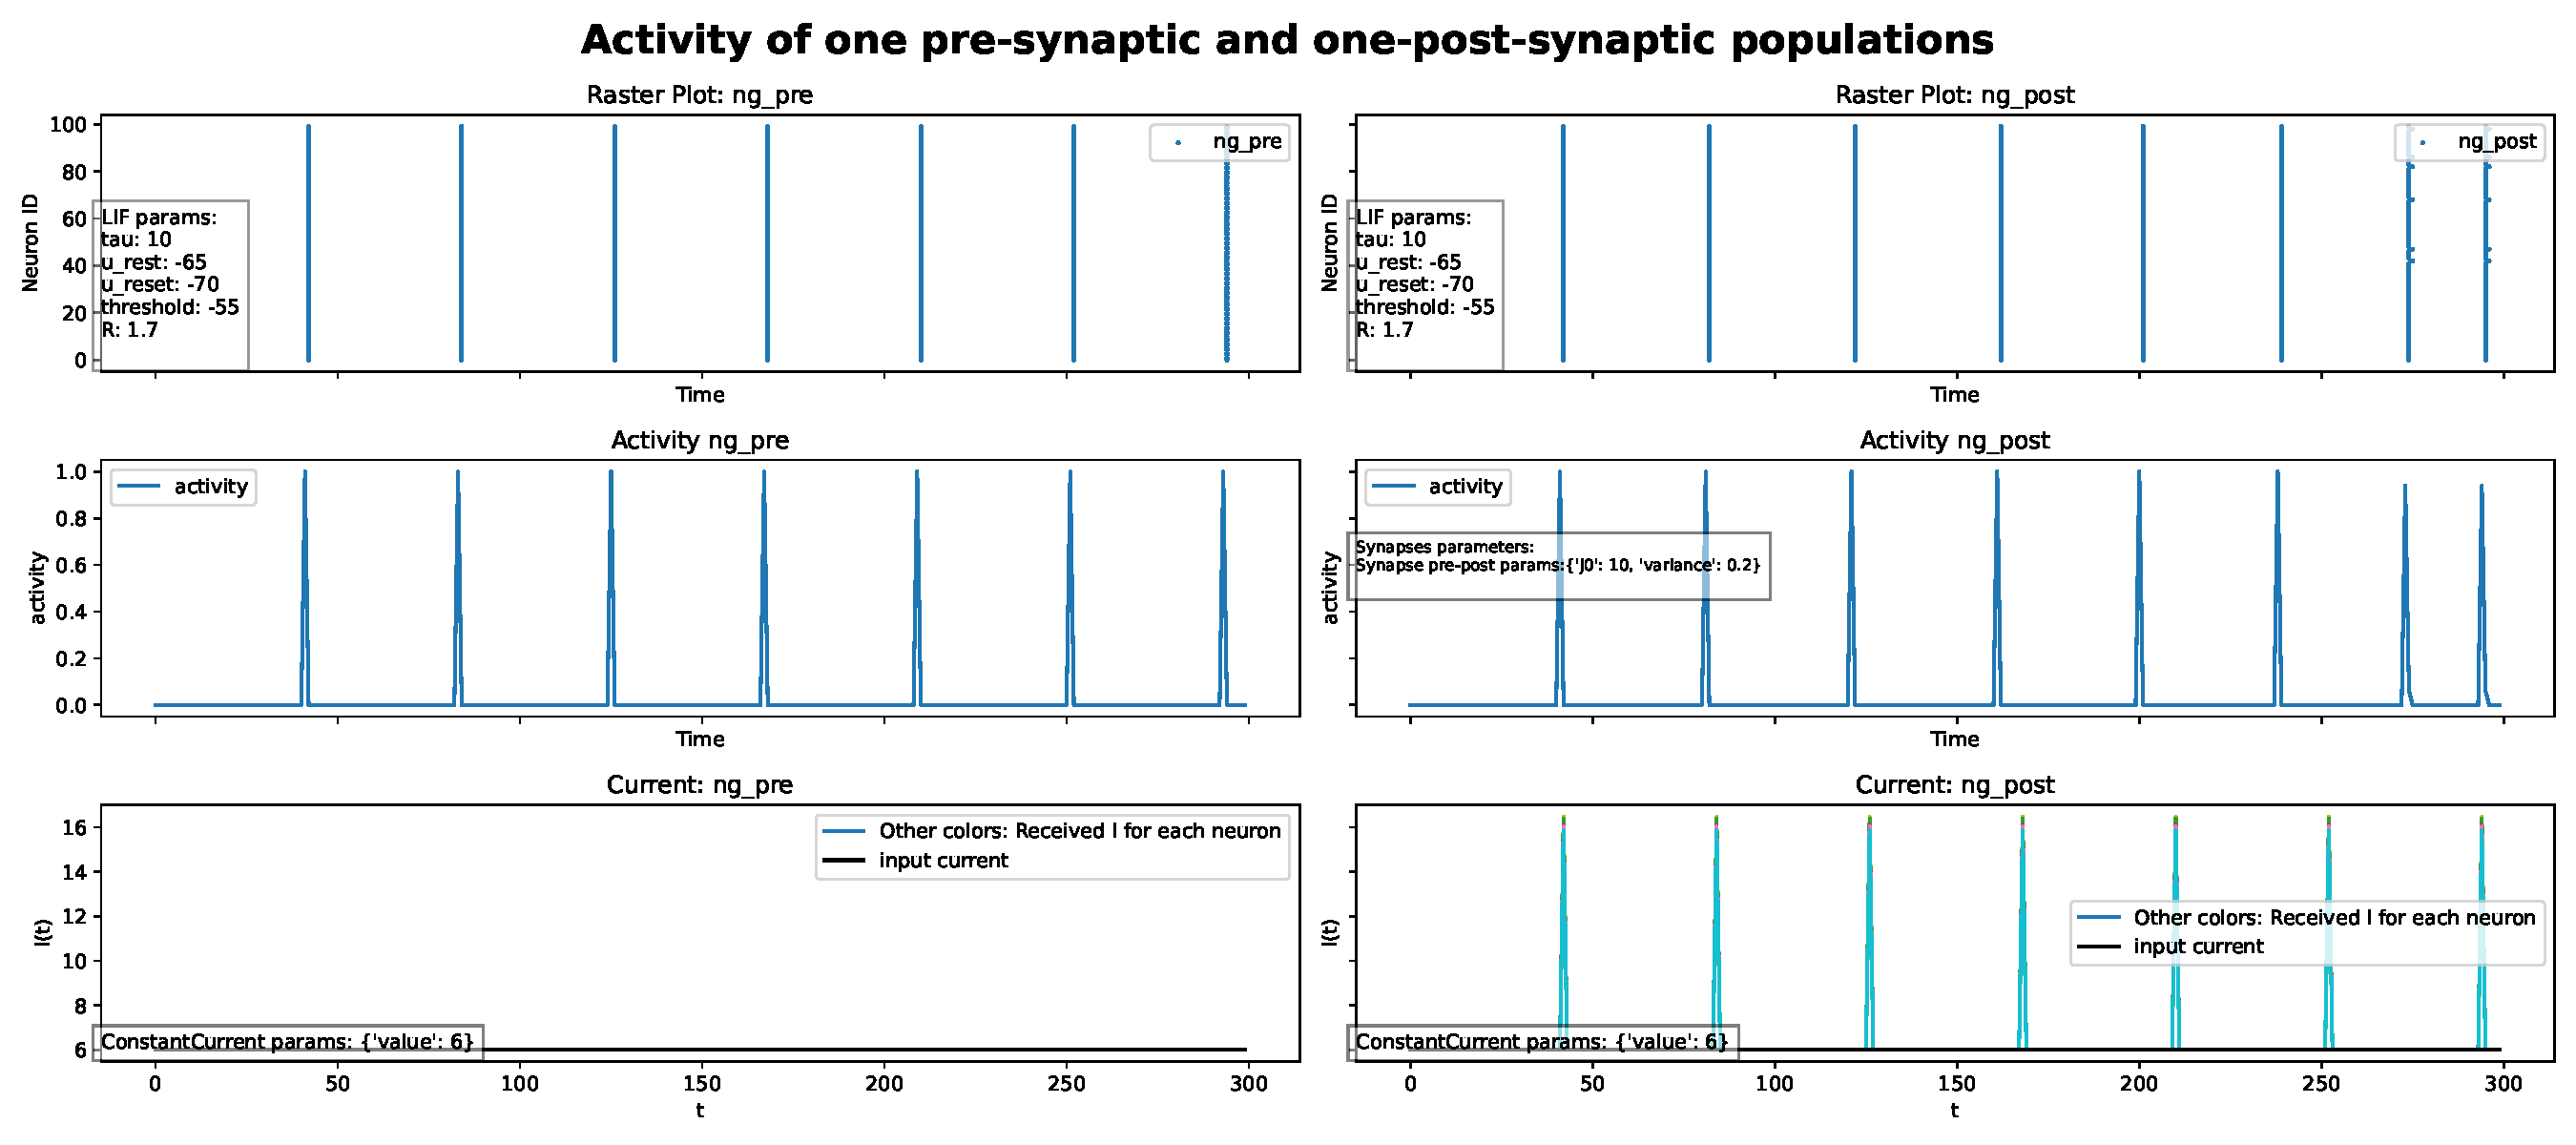
\includegraphics[width=0.9\textwidth]{plots/part1-two-ng-with-synapse.pdf} 
            \caption{جمعیت نورونی پیش سیناپسی و پس سیناپسی}
            \label{fig:part1-two-ng-with-synapse}
        \end{figure}
        \begin{figure}[!ht]
            \centering
            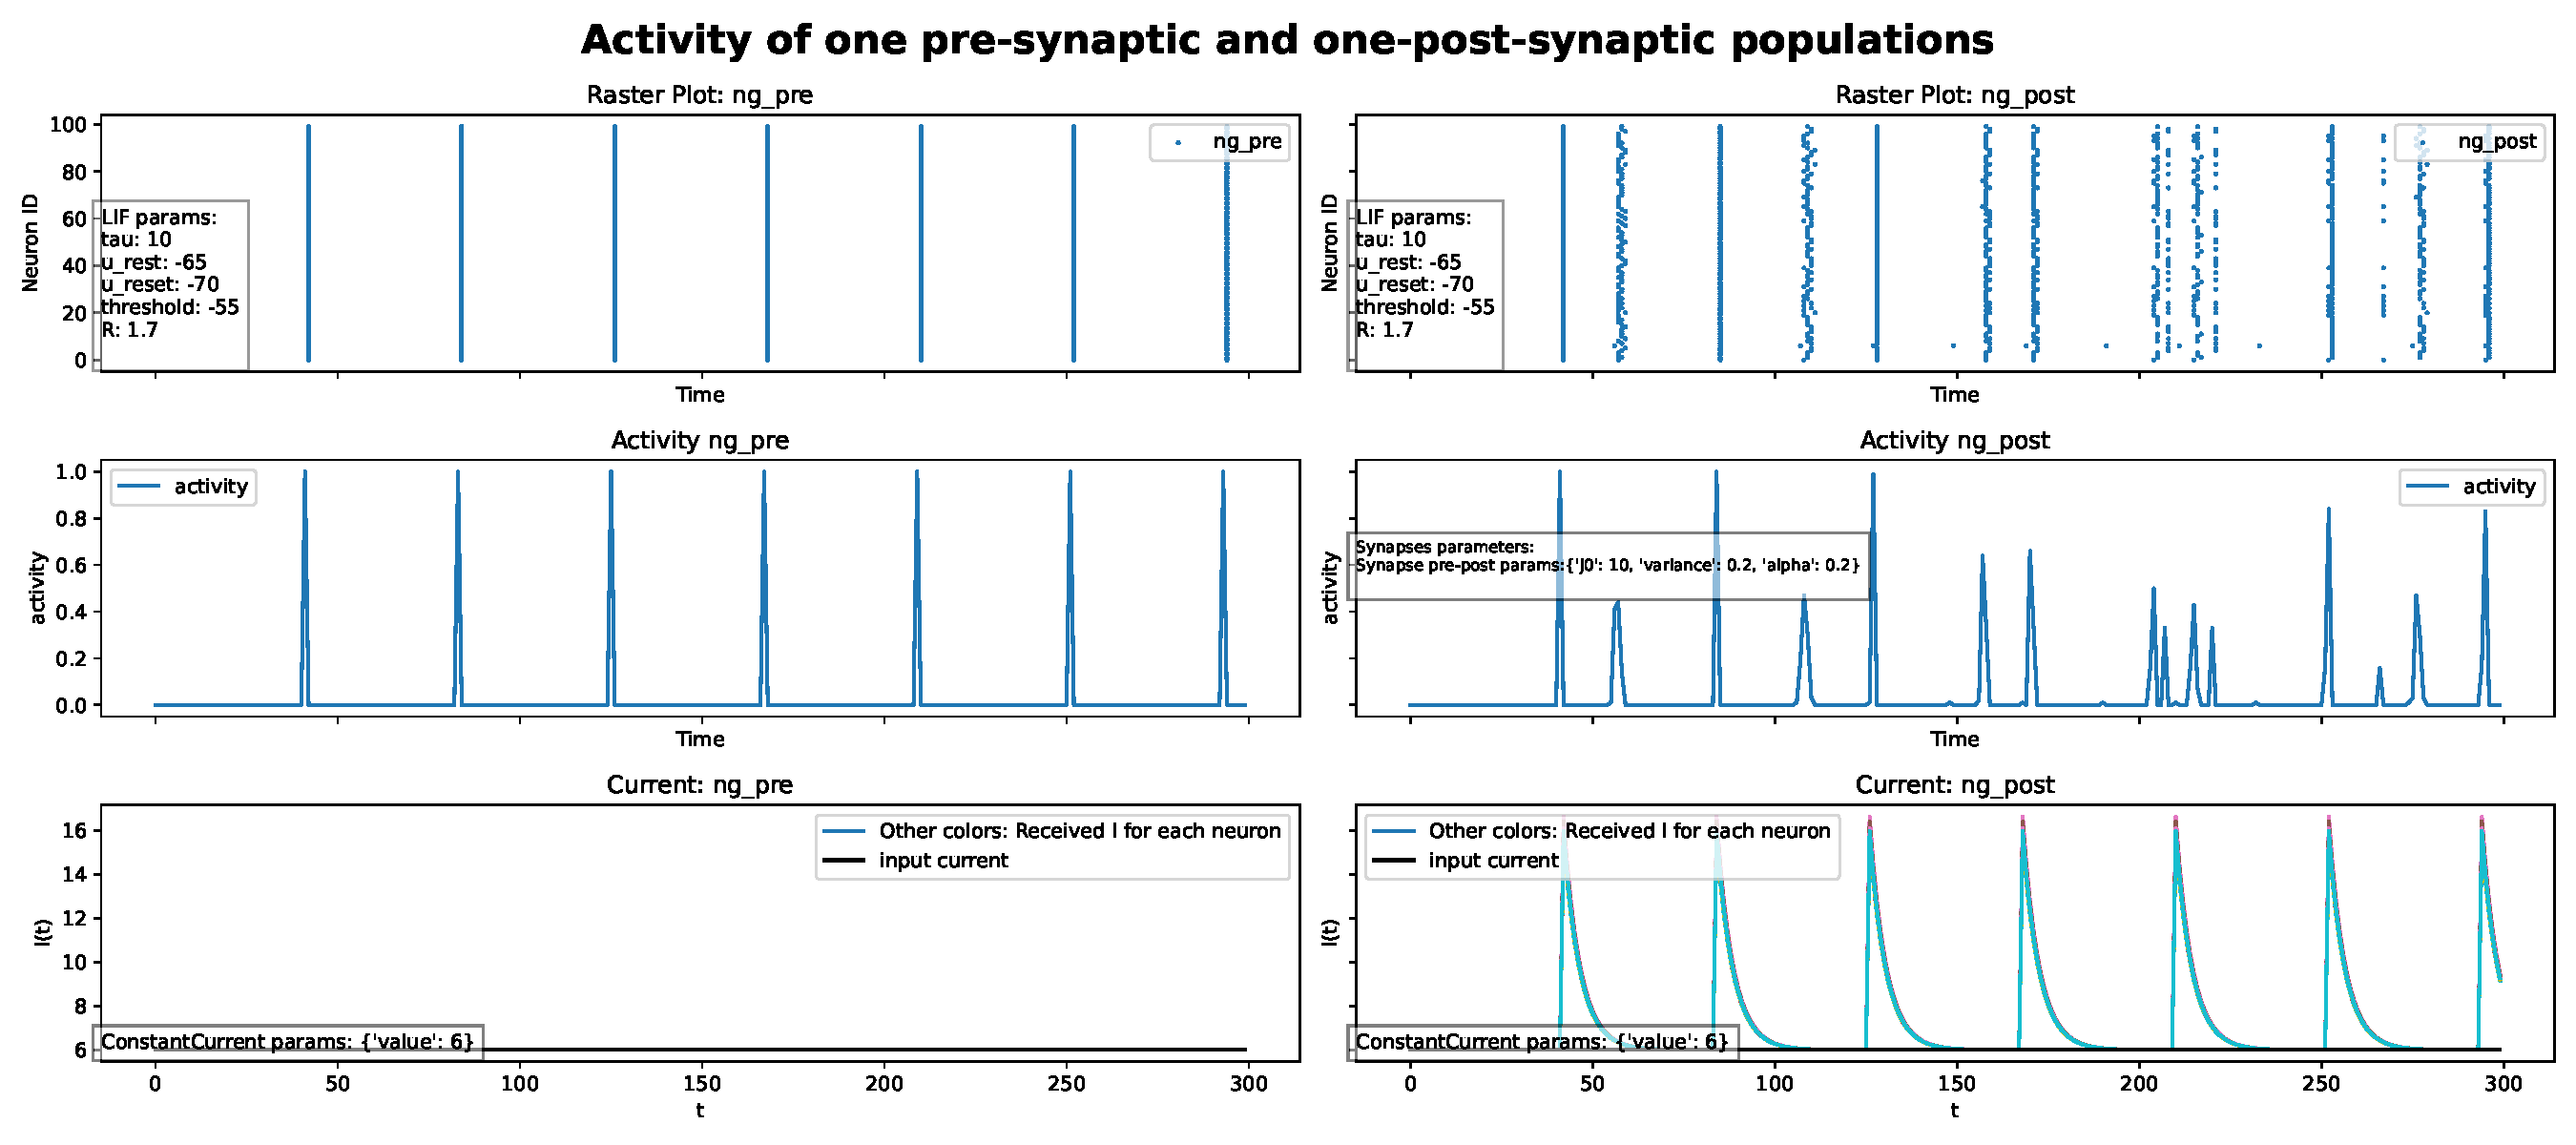
\includegraphics[width=0.9\textwidth]{plots/part1-two-ng-with-synapse-decay.pdf} 
            \caption{جمعیت نورونی پیش سیناپسی و پس سیناپسی: حفظ تاثیر جریان سیناپسی تا لحظات بعد}
            \label{fig:part1-two-ng-with-synapse-decay}
        \end{figure}
        به دلیل اینکه این نوع سیناپس هدف اصلی پروژه نمی باشد، ما بررسی های خود را بیشتر روی همان حالت گفته شده توسط دستیار آموزشی انجام می دهیم.
        
        حال اگر به نمودار 
        \ref{fig:part1-two-ng-with-synapse}
        اختلاف پتانسیل اولیه متفاوت بیفزاییم، طبق شکل 
        \ref{fig:part1-two-ng-with-synapse-u-init}
        ملاحظه میکنیم که فواصل زمانی ضربه ها در جمعیت دوم نزدیک تر بوده و فعالیت آن نسبت به جمعیت اول بیشتر است. این به این دلیل است که در جمعیت دوم، علاوه بر جریان ورودی، جریان سیناپسی که از جمعیت اول گرفته می شود نیز وجود دارد.
        \begin{figure}[!ht]
            \centering
            \includegraphics[width=0.9\textwidth]{plots/part1-two-ng-with-synapse-u\_init.pdf} 
            \caption{جمعیت نورونی پیش سیناپسی و پس سیناپسی: تاثیر اختلاف پتانسیل اولیه متفاوت}
            \label{fig:part1-two-ng-with-synapse-u-init}
        \end{figure}

        حال به جریان ورودی هر دو جمعیت، یک جریان یکسان نویز دار اضافه میکنیم. همانطور که در شکل
        \ref{fig:part1-two-ng-with-synapse-noise-curr}
        ملاحظه میکنیم، با اینکه نویز اضافه شده به هر دو نمودار از توزیع یکسان
        (میانگین=۰ و واریانس=۱)
        پیروی میکند، جریان دریافتی نهایی نورون های جمعیت پس سیناپسی، به طور میانگین بیشتر از جمعیت نورونی پیش سیناپسی است و در نتیجه فعالیت جمعیت آن نیز بیشتر است. این به این دلیل است که جریانی تحت تاثیر ضربه های جمعیت پیش سیناپسی به جریان جمعیت پس سیناپسی نیز اضافه می شود.
        \begin{figure}[!ht]
            \centering
            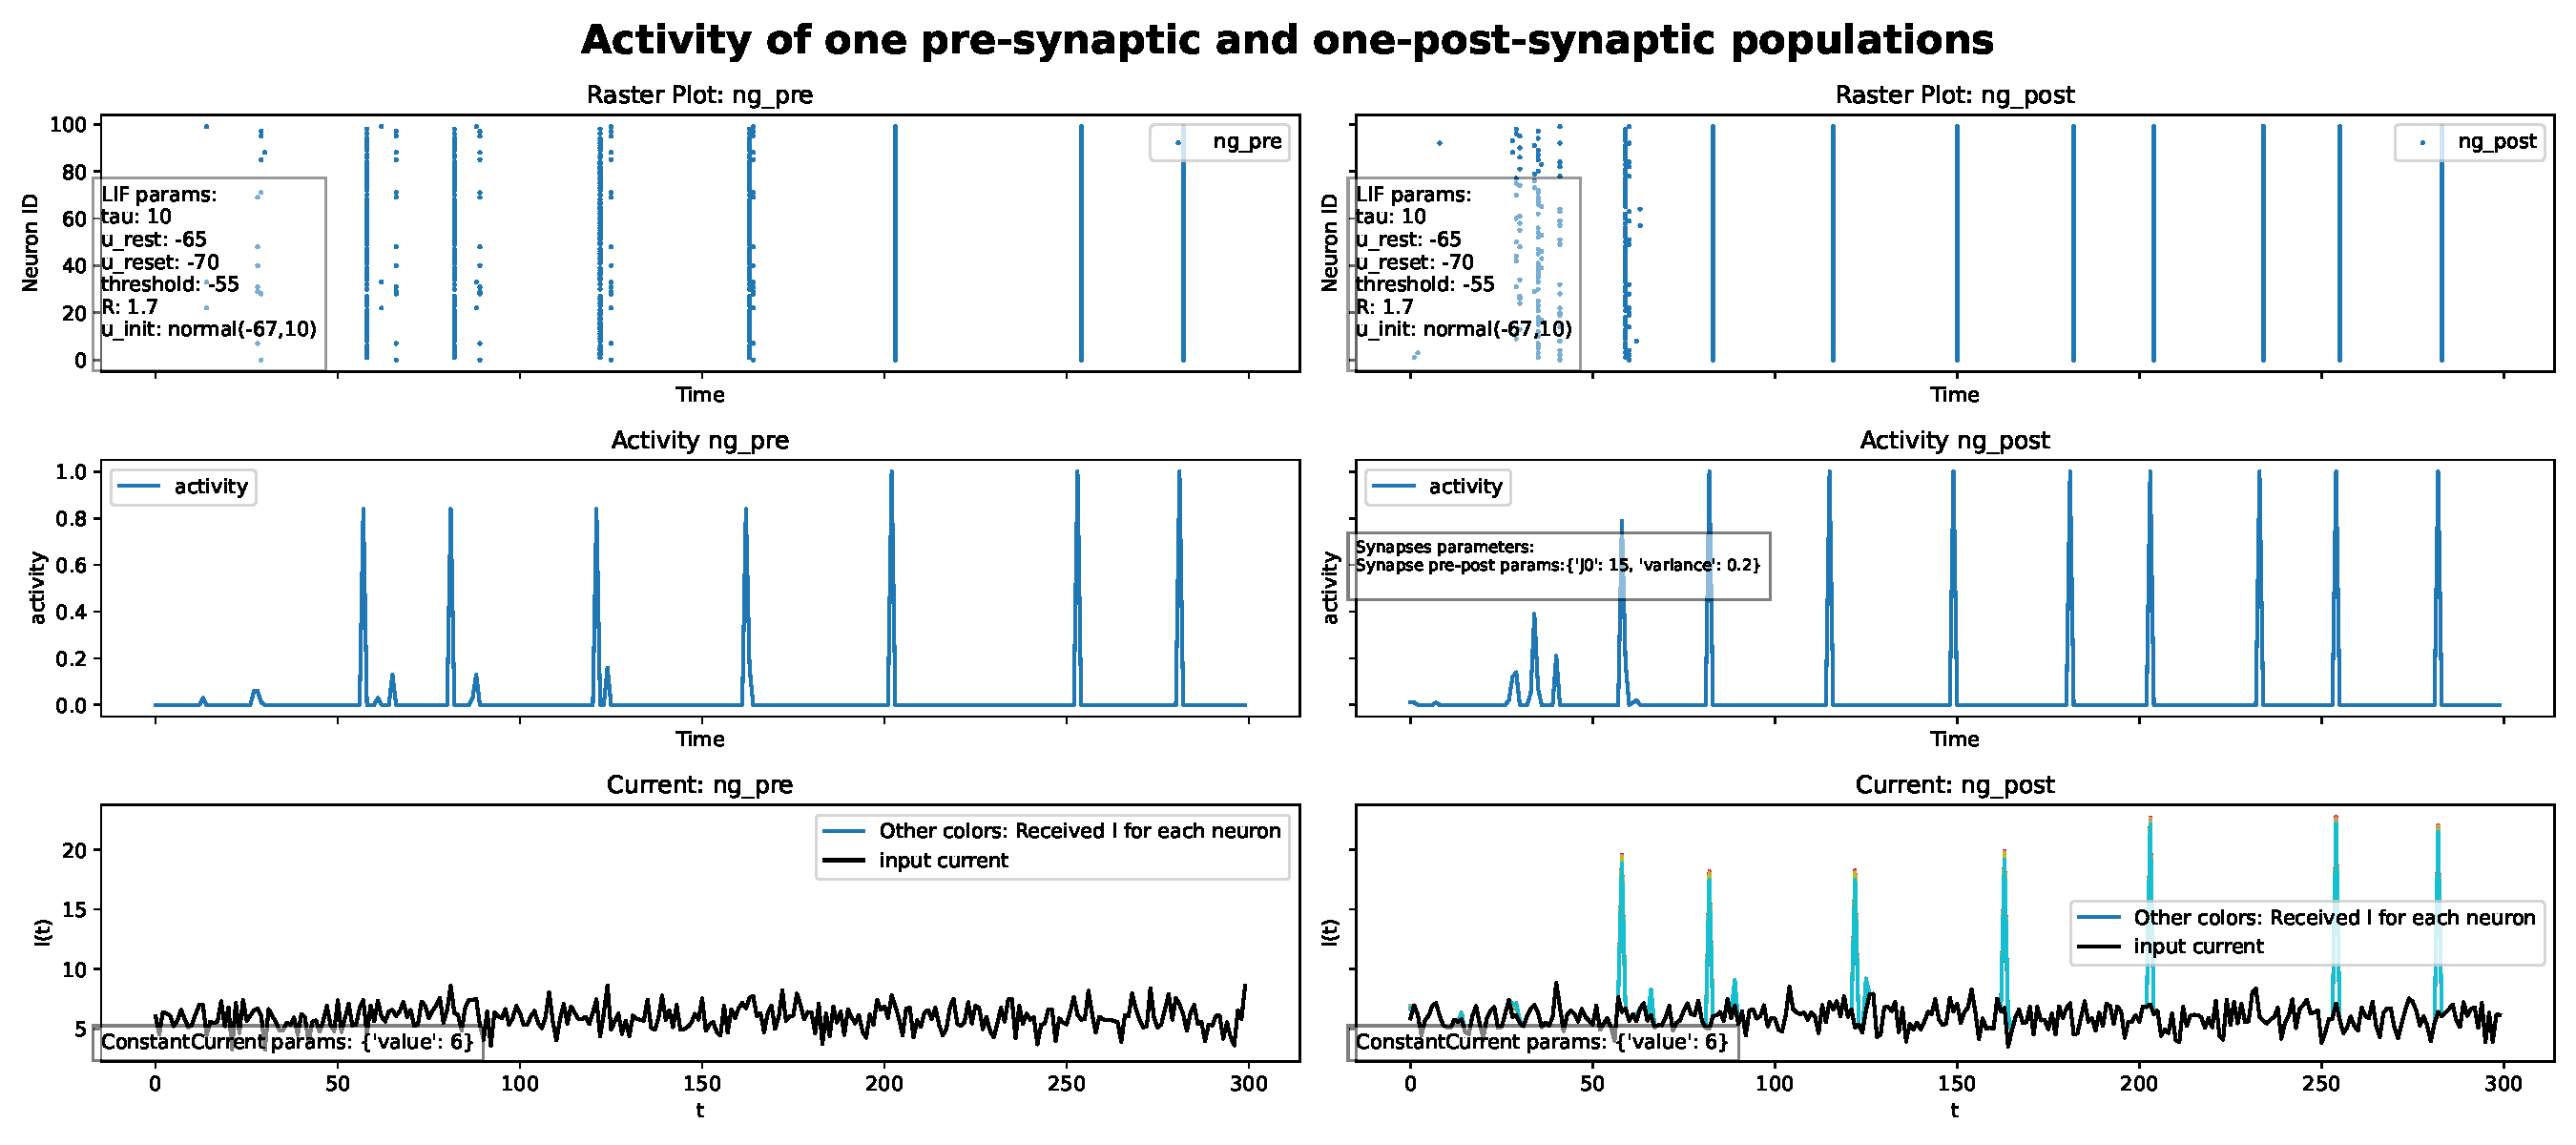
\includegraphics[width=0.9\textwidth]{plots/part1-two-ng-with-synapse-noise-curr.pdf} 
            \caption{جمعیت نورونی پیش سیناپسی و پس سیناپسی: تاثیر جریان نویزی}
            \label{fig:part1-two-ng-with-synapse-noise-curr}
        \end{figure}

        حال رفتار جمعیت را با جریان نویزی غیریکسان آزمایش میکنیم. دامنه نوسان را 
        $0.2$ 
        تنظیم میکنیم و انتظار داریم که مانند شکل های گذشته، میزان پراکندگی زمان ضربه زدن های نورون ها بیشتر شود، که از شکل 
        \ref{fig:part1-two-ng-with-synapse-diff-curr}
        نیز همین دریافت می شود.
        \begin{figure}[!ht]
            \centering
            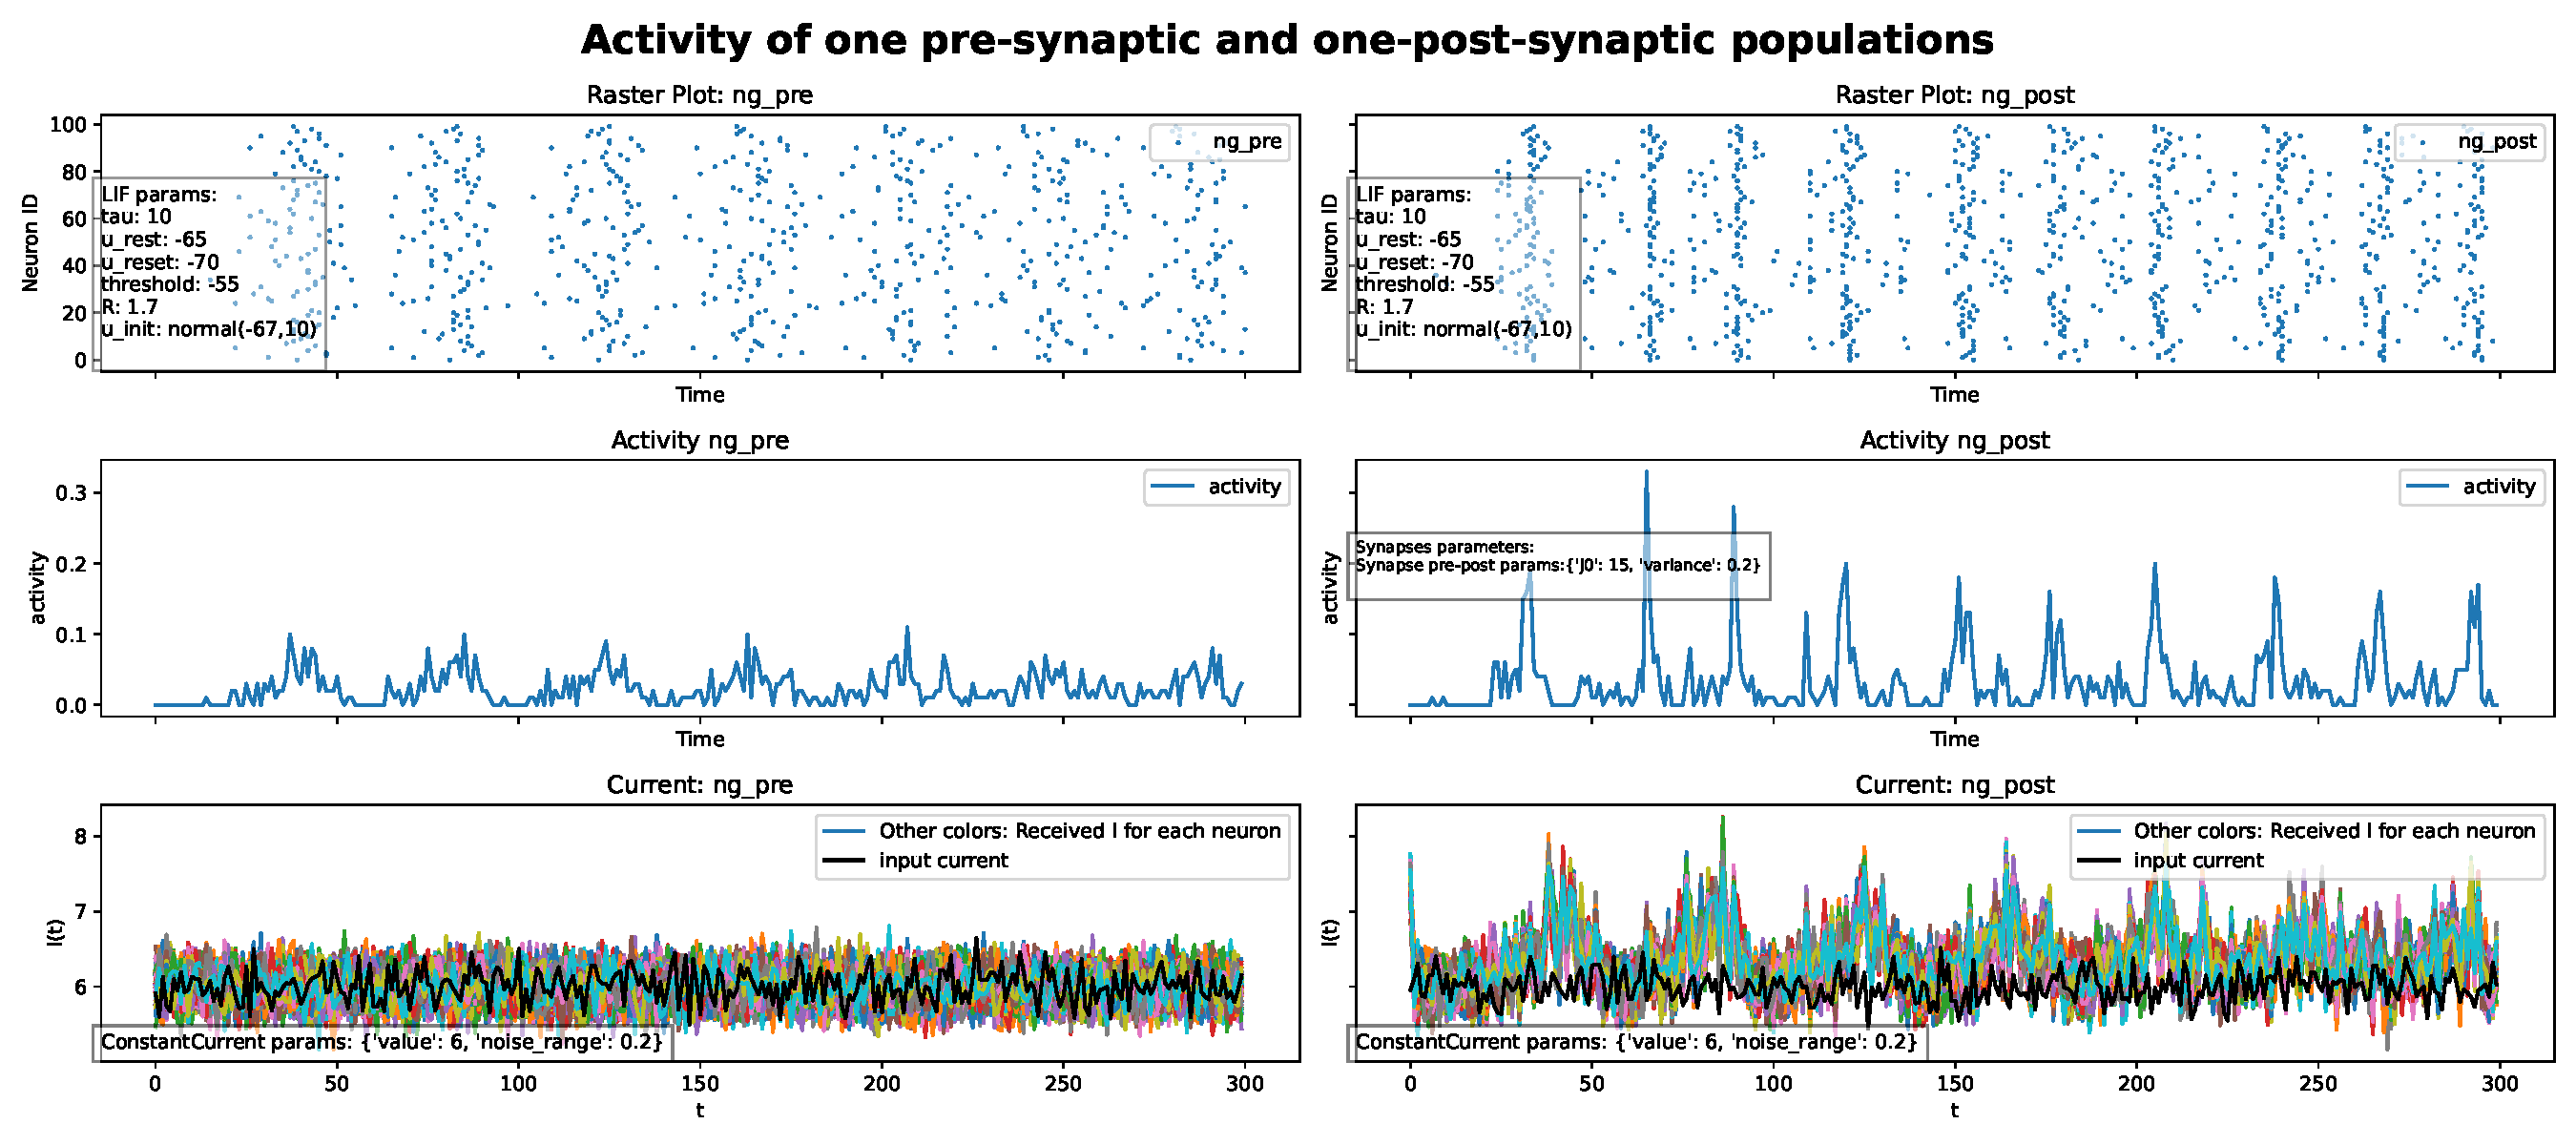
\includegraphics[width=0.9\textwidth]{plots/part1-two-ng-with-synapse-diff-curr.pdf} 
            \caption{جمعیت نورونی پیش سیناپسی و پس سیناپسی: تاثیر جریان نویزی غیریکسان}
            \label{fig:part1-two-ng-with-synapse-diff-curr}
        \end{figure}

        اگر دامنه نوسان جریان را تا 
        $0.5$ 
        بیشتر افزایش دهیم، هرچند پراکندگی زمان ضربه زدن هر دو جمعیت بیشتر می شود، ولی هنوز بیشتر بودن فعالیت جمعیت نورونی دوم مشهود است.
        (شکل \ref{fig:part1-two-ng-with-synapse-high-diff-curr})
        \begin{figure}[!ht]
            \centering
            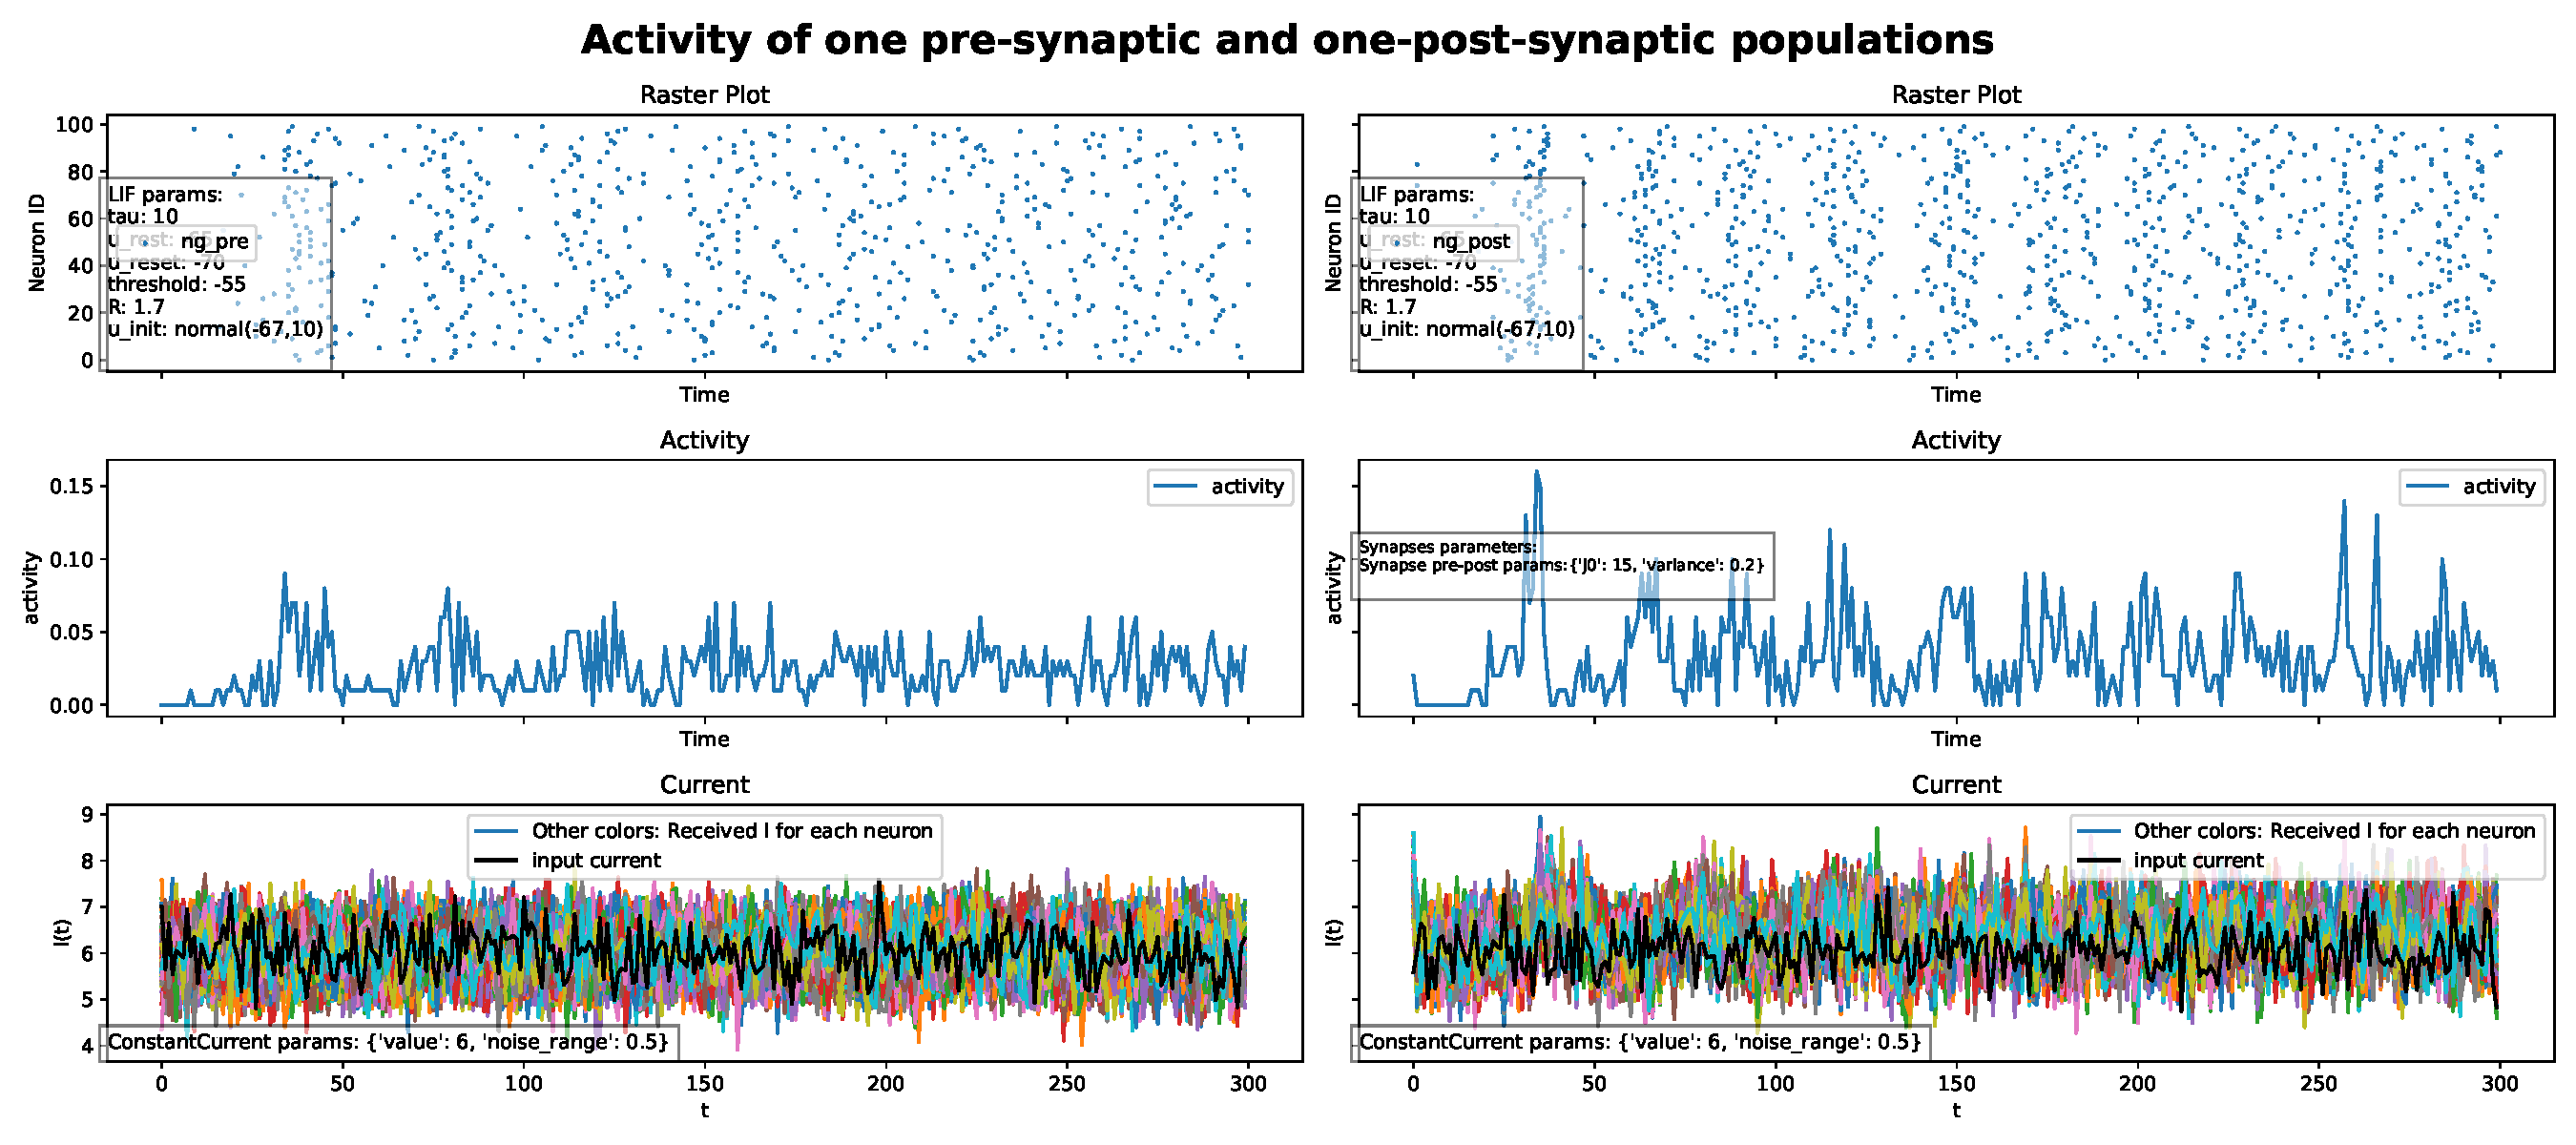
\includegraphics[width=0.9\textwidth]{plots/part1-two-ng-with-synapse-high-diff-curr.pdf} 
            \caption{جمعیت نورونی پیش سیناپسی و پس سیناپسی: تاثیر جریان نویزی غیریکسان}
            \label{fig:part1-two-ng-with-synapse-high-diff-curr}
        \end{figure}
 
        به عنوان آخرین نمودار این بخش و مقدمه ای بر بخش بعدی، افزایش مقدار 
        $j_0$ 
        را بررسی میکنیم. همانطور که از شکل 
        \ref{fig:part1-two-ng-with-synapse-high-diff-curr-high-j}
        بر می آید، افزایش 
        $j_0$ 
        منجر به افزایش وزن ها و در نتیجه افزایش جریان سیناپسی ورودی به جمعیت نورونی پس سیناپسی شده و فعالیت آن را بیشتر می کند.
        \begin{figure}[!ht]
            \centering
            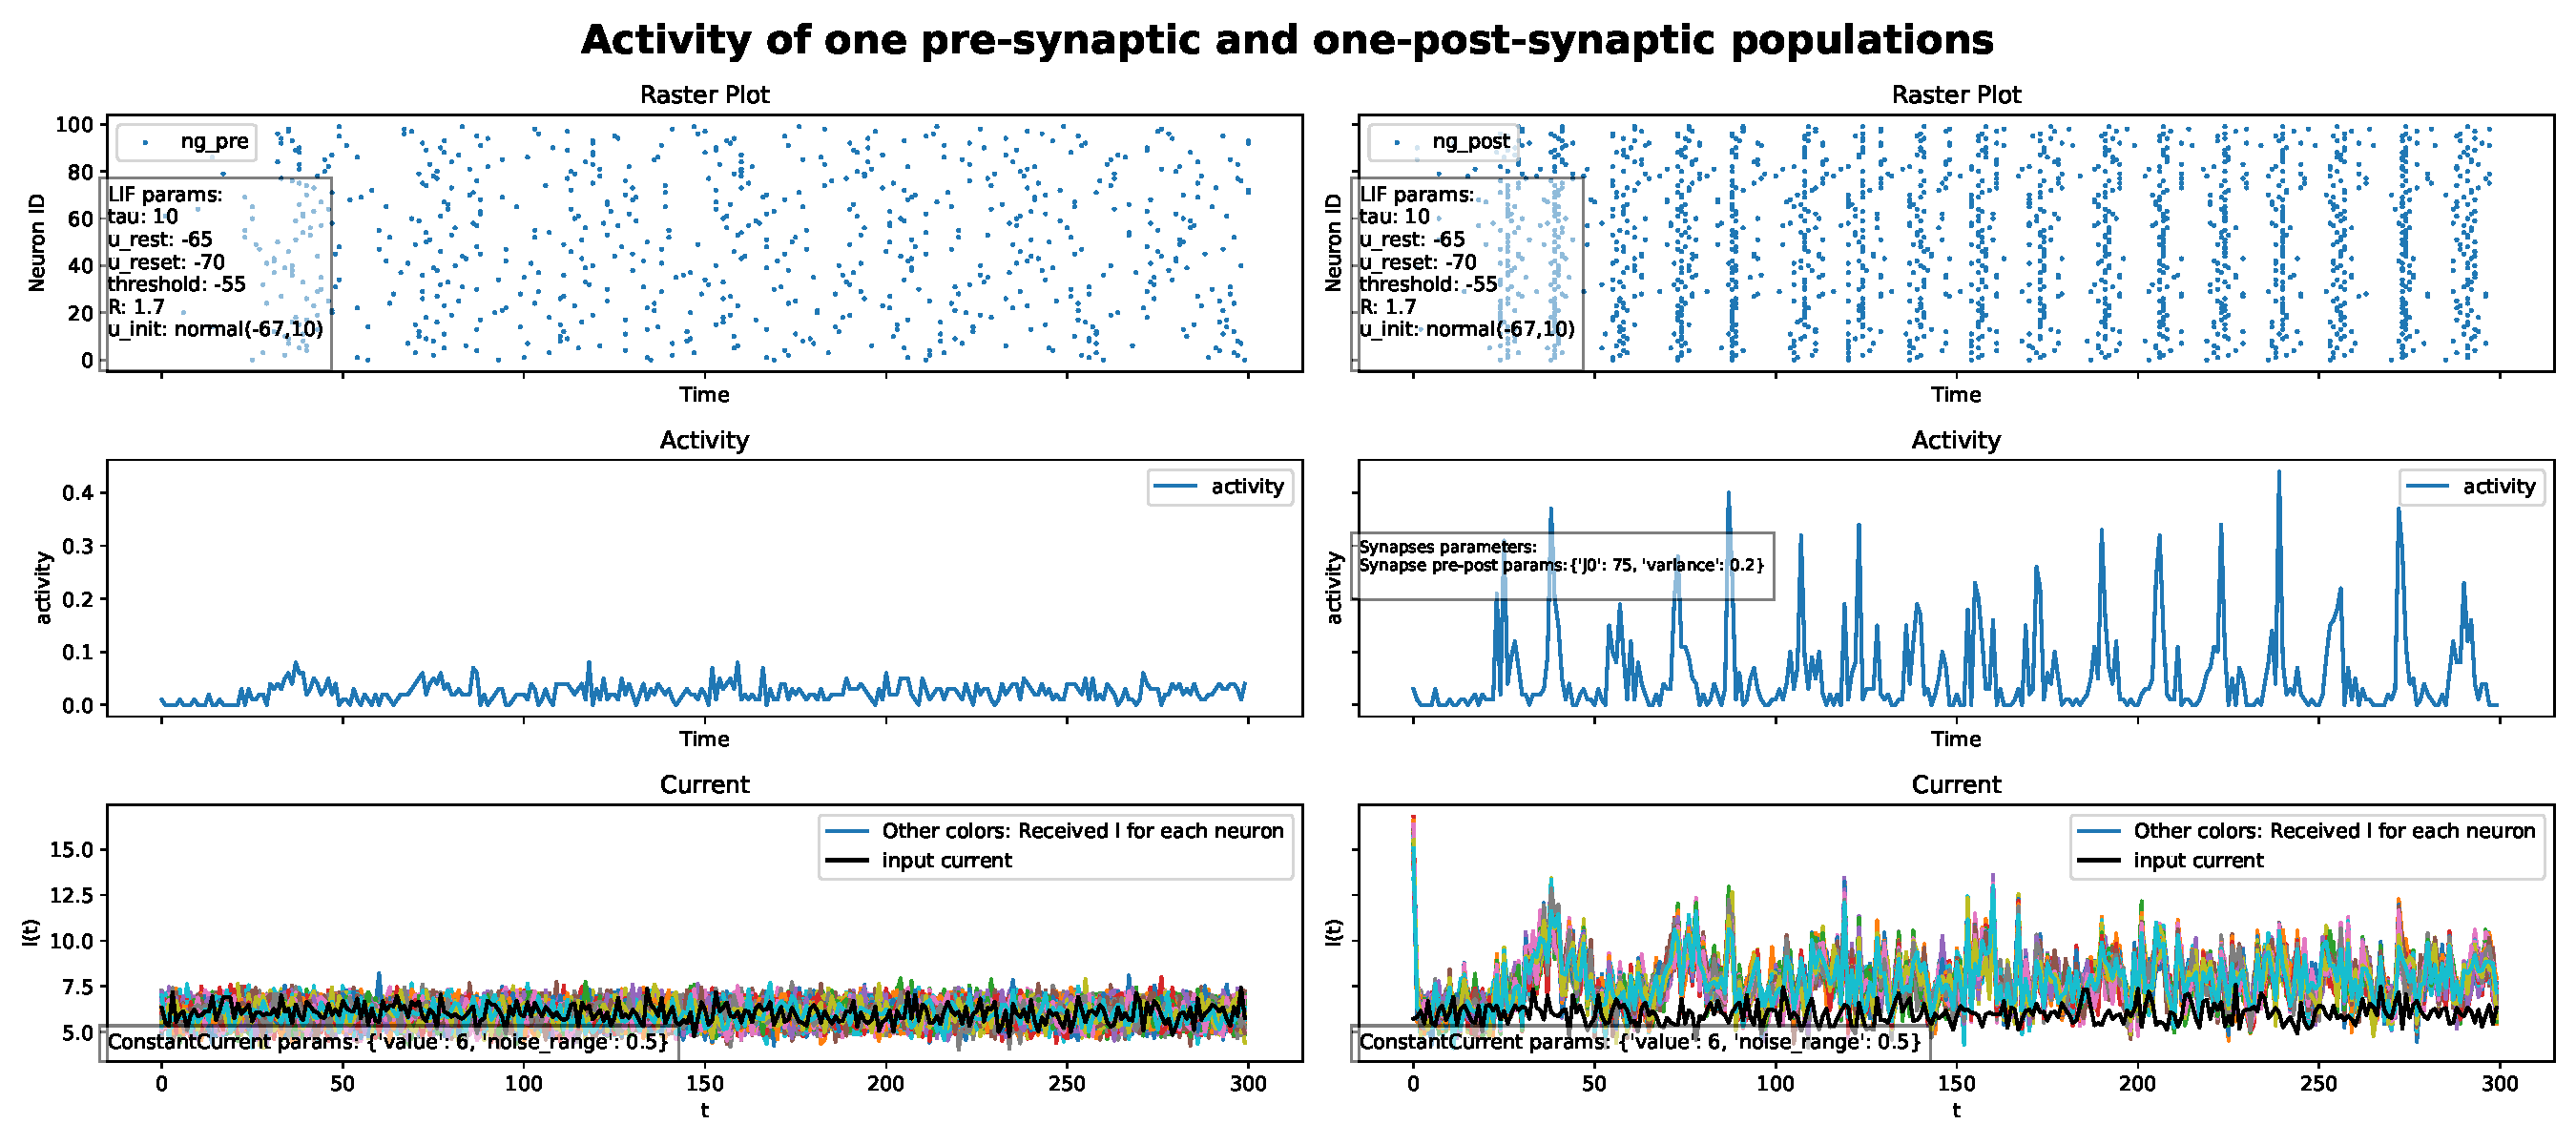
\includegraphics[width=0.9\textwidth]{plots/part1-two-ng-with-synapse-high-diff-curr-high-j.pdf} 
            \caption{جمعیت نورونی پیش سیناپسی و پس سیناپسی: تاثیر جریان نویزی غیریکسان}
            \label{fig:part1-two-ng-with-synapse-high-diff-curr-high-j}
        \end{figure}

\newpage
\section{الگو های ارتباطی}
    در این بخش از پروژه، به بررسی سه الگوی متفاوت ارتباطی، یعنی الگوی ارتباط کامل
    \footnote{\lr{Full connectivity}}، 
    ارتباط تصادفی با احتمال جفت شدن ثابت
    \footnote{\lr{Random coupling: Fixed coupling probability}}
    و ارتباط تصادفی با تعداد ثابت نورون پیش سیناپسی
    \footnote{\lr{Random coupling: Fixed number of presynaptic partners}}
    می پردازیم. در این بخش، با انجام آزمایش های مناسب، جریان حاصل و حساسیت به نویز را در هر یک از این الگو ها بررسی میکنیم.

    ارتباط واقعی بین نورون‌های قشری انواع مختلف و لایه‌های مختلف، یا درون گروه‌هایی از نورون‌های هم نوع و یک لایه هنوز تا حدی ناشناخته است، زیرا داده‌های تجربی محدود است. حداکثر، برخی برآوردهای قابل قبول از احتمالات اتصال وجود دارد. در برخی موارد احتمال اتصال به عنوان وابسته به فاصله در نظر گرفته می شود، در سایر تخمین های تجربی به عنوان یکنواخت در همسایگی محدود یک ستون
    ($column$)
    قشر مغز.

    در شبیه‌سازی های ما چند طرح جفت وجود دارد که اغلب مورد استفاده قرار می‌گیرند. اکثر اینها اتصال تصادفی درون و بین جمعیت ها را فرض می کنند. در ادامه این طرح‌ها را با تمرکز ویژه بر رفتار مقیاس‌بندی ناشی از هر انتخاب از طرح‌های جفت مورد بحث قرار می‌دهیم. در اینجا، رفتار مقیاس‌بندی به تغییر در تعداد 
    $N$
    نورون‌هایی که در جمعیت شرکت می‌کنند اشاره دارد.
    \cite{Neuronal-Dynamics}
    \subsection{الگوی ارتباط کامل}
        ساده ترین الگوی ارتباط، اتصال همه-به-همه در یک جمعیت است. همه اتصالات وزن یکسانی دارند. اگر بخواهیم تعداد 
        $N$
        نورون‌ها را در شبیه‌سازی یک جمعیت تغییر دهیم، یک فرمول مقیاس‌بندی مناسب، فرمول 
        $w_{ij} = \frac{j_0}{N}$
        است.

        این فرمول مقیاس‌بندی یک انتزاع ریاضی است که ما را قادر می‌سازد تا به طور فرمال حد 
        $\lim_{N\rightarrow \infty}$
        را بگیریم و در عین حال ورودی مورد انتظاری را که یک نورون از نورون های پیش سیناپسی خود در جمعیت دریافت می‌کند ثابت نگه داریم. در حد حد 
        $\lim_{N\rightarrow \infty}$
        ، نوسانات ناپدید می شوند و ورودی مورد انتظار را می توان به عنوان ورودی واقعی هر یک از نورون های 
        $N$ 
        در نظر گرفت. البته جمعیت های واقعی اندازه محدودی دارند، به طوری که همیشه برخی از نوسانات باقی می ماند. اما با افزایش 
        $N$
        نوسانات کاهش می یابد. \cite{Neuronal-Dynamics}
        
        حال به شبیه سازی و بررسی این ارتباط می پردازیم. در این قسمت، یکبار برای یک جمعیت و یکبار برای دو جمعیت، آزمایش هایمان را انجام می دهیم. از آنجا که تاثیر برخی پارامتر ها را در بخش قبل انجام دادیم، در این قسمت بیشتر روی آزمایش پارامتر های خود سیناپس ها متمرکز می شویم.
        \subsubsection*{بررسی رفتار یک جمعیت}
            برای بررسی رفتار رو یک جمعیت، کافی است که یک جمعیت نورونی به همراه سیناپس داخل آن تشکیل داده و آن را شبیه سازی کنیم. از آنجا که در بخش اول، تاثیر جریان نویز دار و همچنین اختلاف پتانسیل اولیه در آورده شده است، از بررسی دوباره آن ها در اینجا خودداری می شود و پارامتر های خود سیناپس مورد تحلیل قرار میگیرد. از این رو، 
            برای شروع، یک جمعیت نورونی با مدل 
            $LIF$
            (\lr{Leaky-integrate-and-fire})
            \footnote{مدل تجمیع و آتش نشتی}
            با پارامتر های 
            $\tau=10$,
            $u_{rest}=-65$,
            $u_{reset}=-70$,
            $threshold=-55$,
            $R=1.7$,
            $u_{init}=normal(-67,10)$
            و جریان ثابت نویزدار
            $6$ 
            میسازیم. 
            \paragraph{پارامتر $j_0$}
                در ابتدا تاثیر پارامتر 
                $j_0$
                را بر روی رفتار تحلیل میکنیم. برای این منظور، سه مقدار 
                $j_0=5$,
                $j_0=25$,
                $j_0=75$
                را شبیه سازی میکنیم. همچنین پارامتر واریانس را 
                $\tilde{\sigma}=0.25$ 
                میگیریم. از آنجا که فرمول موردنیاز برای واریانس به طور کامل برای هر سه مدل شرح داده نشده بود، به طور کلی برای سه مدل، این پارامتر در مقدار میانگین نهایی
                (فرمول $\frac{j_0}{N}$) 
                ضرب شده و مقدار واریانس در توزیع 
                $normal(\mu,\sigma)$ 
                را می سازد.
                % \begin{equation}
                %     w_{ij}=normal(\mu,\sigma); \mu=\frac{j0}{N}, \sigma=\mu\times\tilde{\sigma}
                % \end{equation}
                همانطور که در شکل 
                \ref{fig:part2-one-ng-full-synapse-diff-j}
                مشاهده میکنیم، با افزایش 
                $j_0$ 
                میزان نواسات کاهش می یابد. تحلیل من از این اتفاق این است که با زیاد شدن مقدار وزن های سیناپسی در یک جمعیت نورونی، بعد از ضربه زدن نورون های یک جمعیت، مقدار جریان حاصل از سیناپس نیز افزایش یافته، و در لحظه بعدی نورون ها جریان بیشتری دریافت کرده و در نتیجه سریع تر ضربه میزنند. از آنجا که سرعت ضربه زدن آن ها افزایش می یابد، تفاوت اختلاف پتانسیل متفاوتی که در مقدار دهی اولیه به آن ها داده شده بود نیز رفته رفته کمتر شده و پس از مدتی زمان ضربه زدن نورون ها نزدیک به یکدیگر می شود. علاوه بر کم شدن پراکندگی لحظات ضربه ها، میبینم که در نمودار سمت راست، نورون ها تعداد ضربه های بیشتری نیز در کل زده اند.
                \begin{figure}[!ht]
                    \centering
                    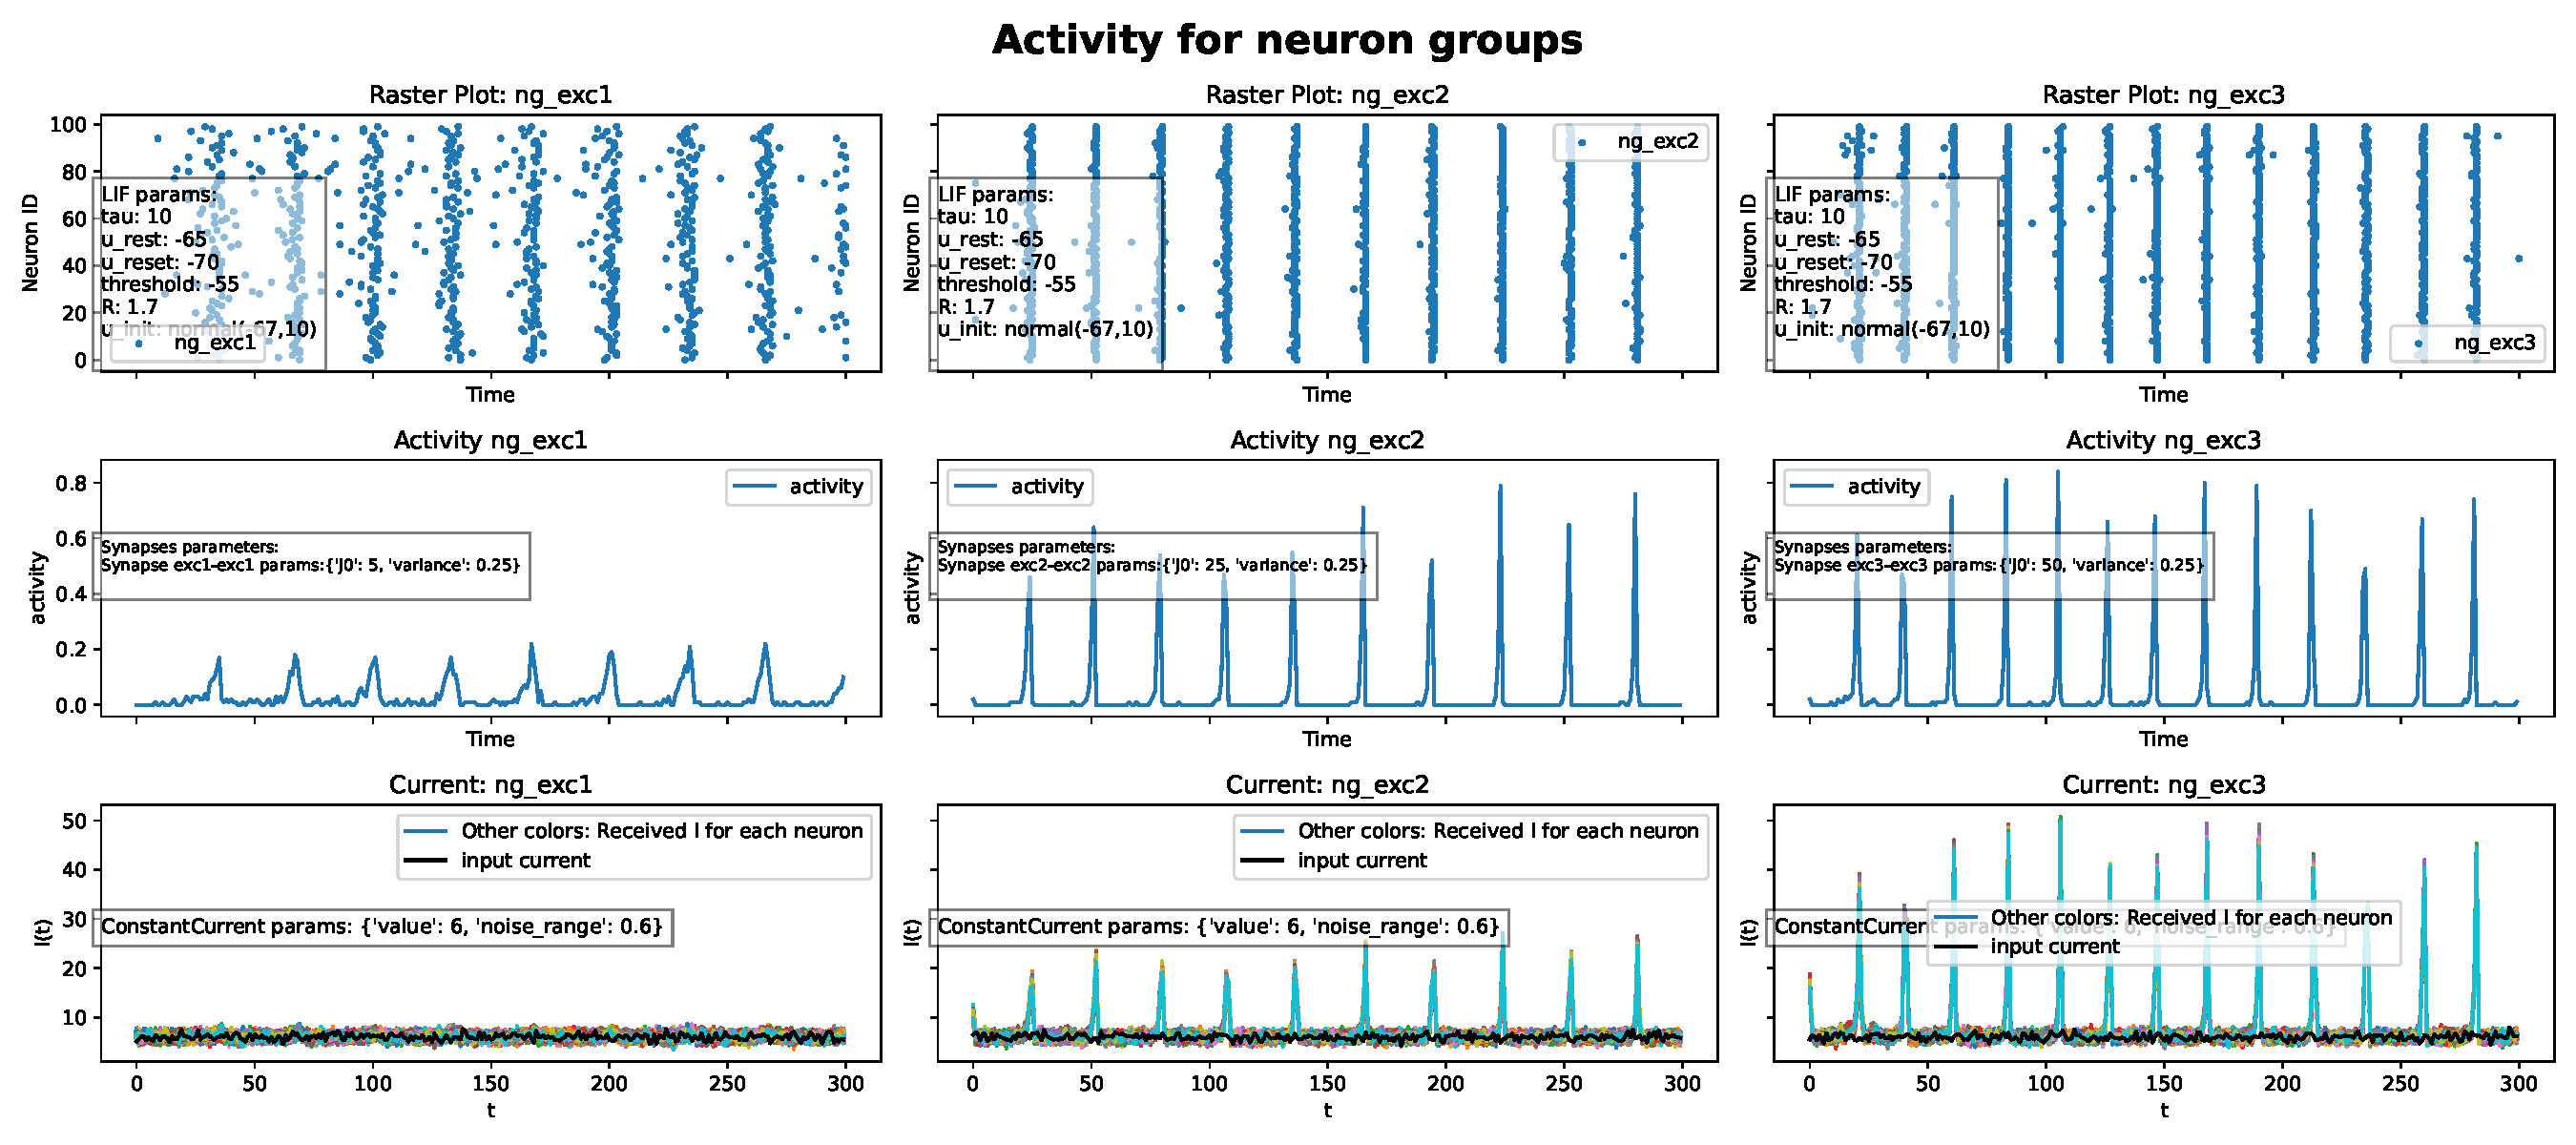
\includegraphics[width=0.9\textwidth]{plots/part2-one-ng-full-synapse-diff-j.pdf} 
                    \caption{رفتار یک جمعیت نورونی با مقادیر $j_0$ مختلف و جریان ثابت نویز دار}
                    \label{fig:part2-one-ng-full-synapse-diff-j}
                \end{figure}

                حال به جمعیت نورونی مان، یک جریان تصادفی میدهیم تا رفتار شبیه به نورون واقعی را بیشتر بررسی کنیم. مجددا در شکل
                \ref{fig:part2-one-ng-full-synapse-diff-j-rand-curr}
                مشاهده میکنیم که تصادفی بودن جریان، منجر به پراکندگی زمان ضربه زدن نورون ها می شود و به طور کلی فعالیت آن ها را کاهش داده است، اما با زیاد کردن وزن های سیناپسی، این نوسانات کمتر شده به طور که در نمودار سمت راست، میتوانیم زمان ضربه زدن نورون ها را در ستون هایی دسته بندی کنیم.
                \begin{figure}[!ht]
                    \centering
                    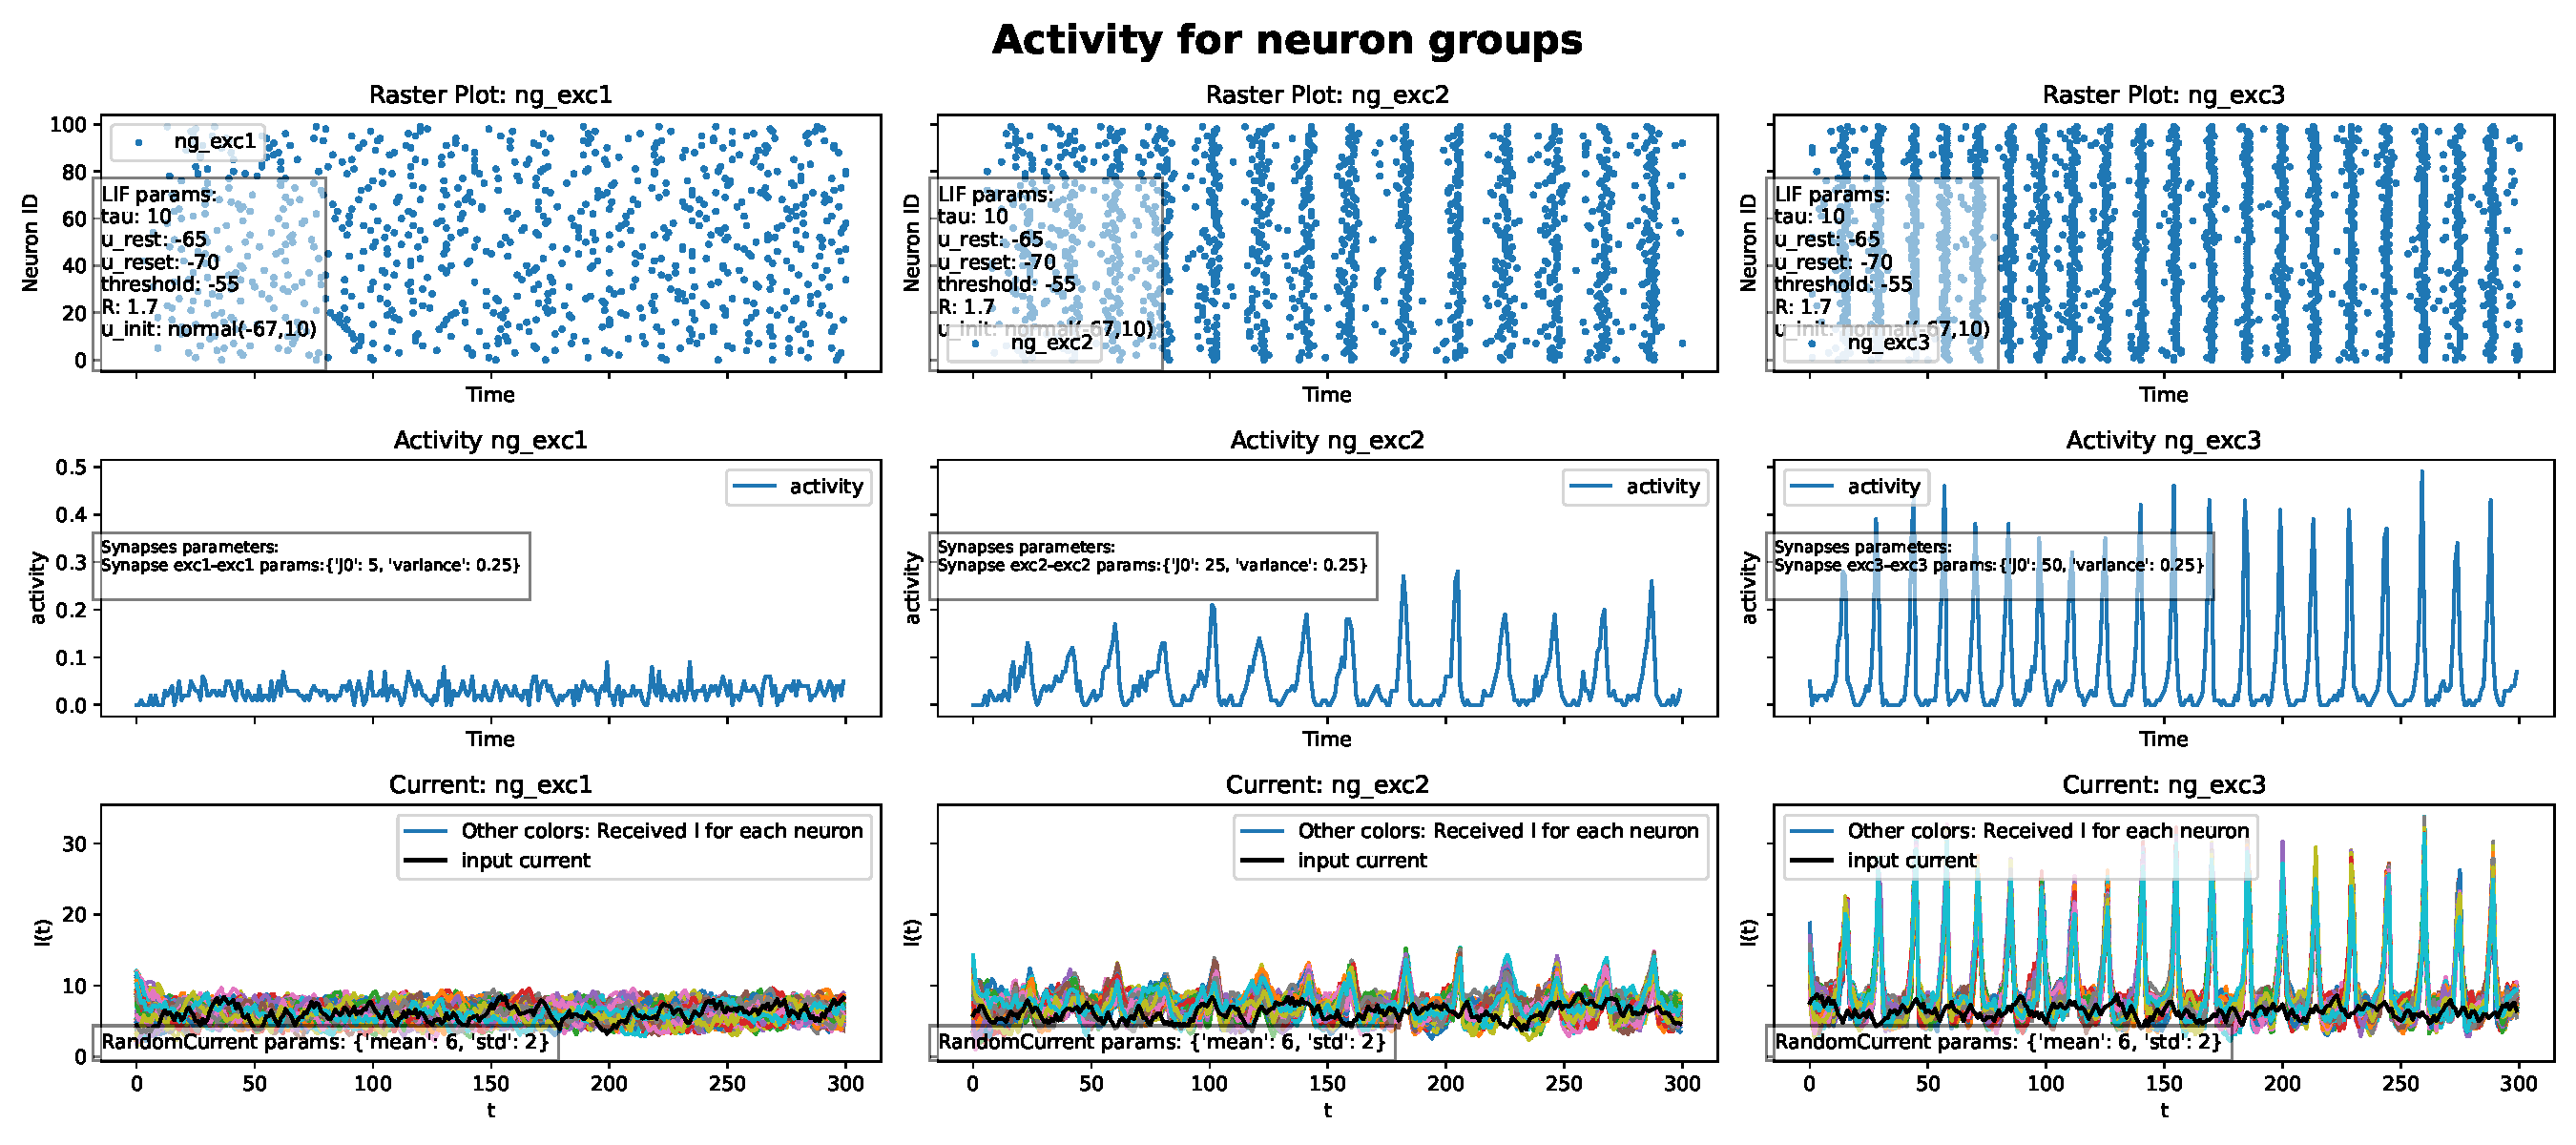
\includegraphics[width=0.9\textwidth]{plots/part2-one-ng-full-synapse-diff-j-rand-curr.pdf} 
                    \caption{رفتار یک جمعیت نورونی با مقادیر $j_0$ مختلف و جریان تصادفی}
                    \label{fig:part2-one-ng-full-synapse-diff-j-rand-curr}
                \end{figure}

            \paragraph*{پارامتر واریانس}
                حال رفتار جمعیت را به ازای مقادیر مختلف واریانس تحلیل میکنیم. برای این قسمت نیز از همان مدل نورونی بالا استفاده میکنیم. از آنجا که الگوی ارتباطی مان کامل است، انتظار داریم که تغییر معقول واریانس تفاوت زیادی در رفتار کلی نورون ها ایجاد نکند، چرا که هر نورون با تمام نورون های دیگر ارتباط دارد و از این رو برآیند جریان سناپسی وارد شده به نورون ها نزدیک به هم می باشد. شکل 
                \ref{fig:part2-one-ng-full-synapse-diff-variance}
                بیانگر همین موضوع است. هر چند تغییرات کوچکی میتواند رخ دهد. مثلا در نمودار سمت راست که واریانس برابر با خود میانگین دارد
                (گفتیم که عددی که به عنوان واریانس به مدل ورودی داده می شود در میانگین ضرب شده و سپس تشکیل واریانس اصلی توزیع را می دهد)،
                میزان فعالیت کلی نورون ها کمی از دو مدل دیگر بیشتر است.
                \begin{figure}[!ht]
                    \centering
                    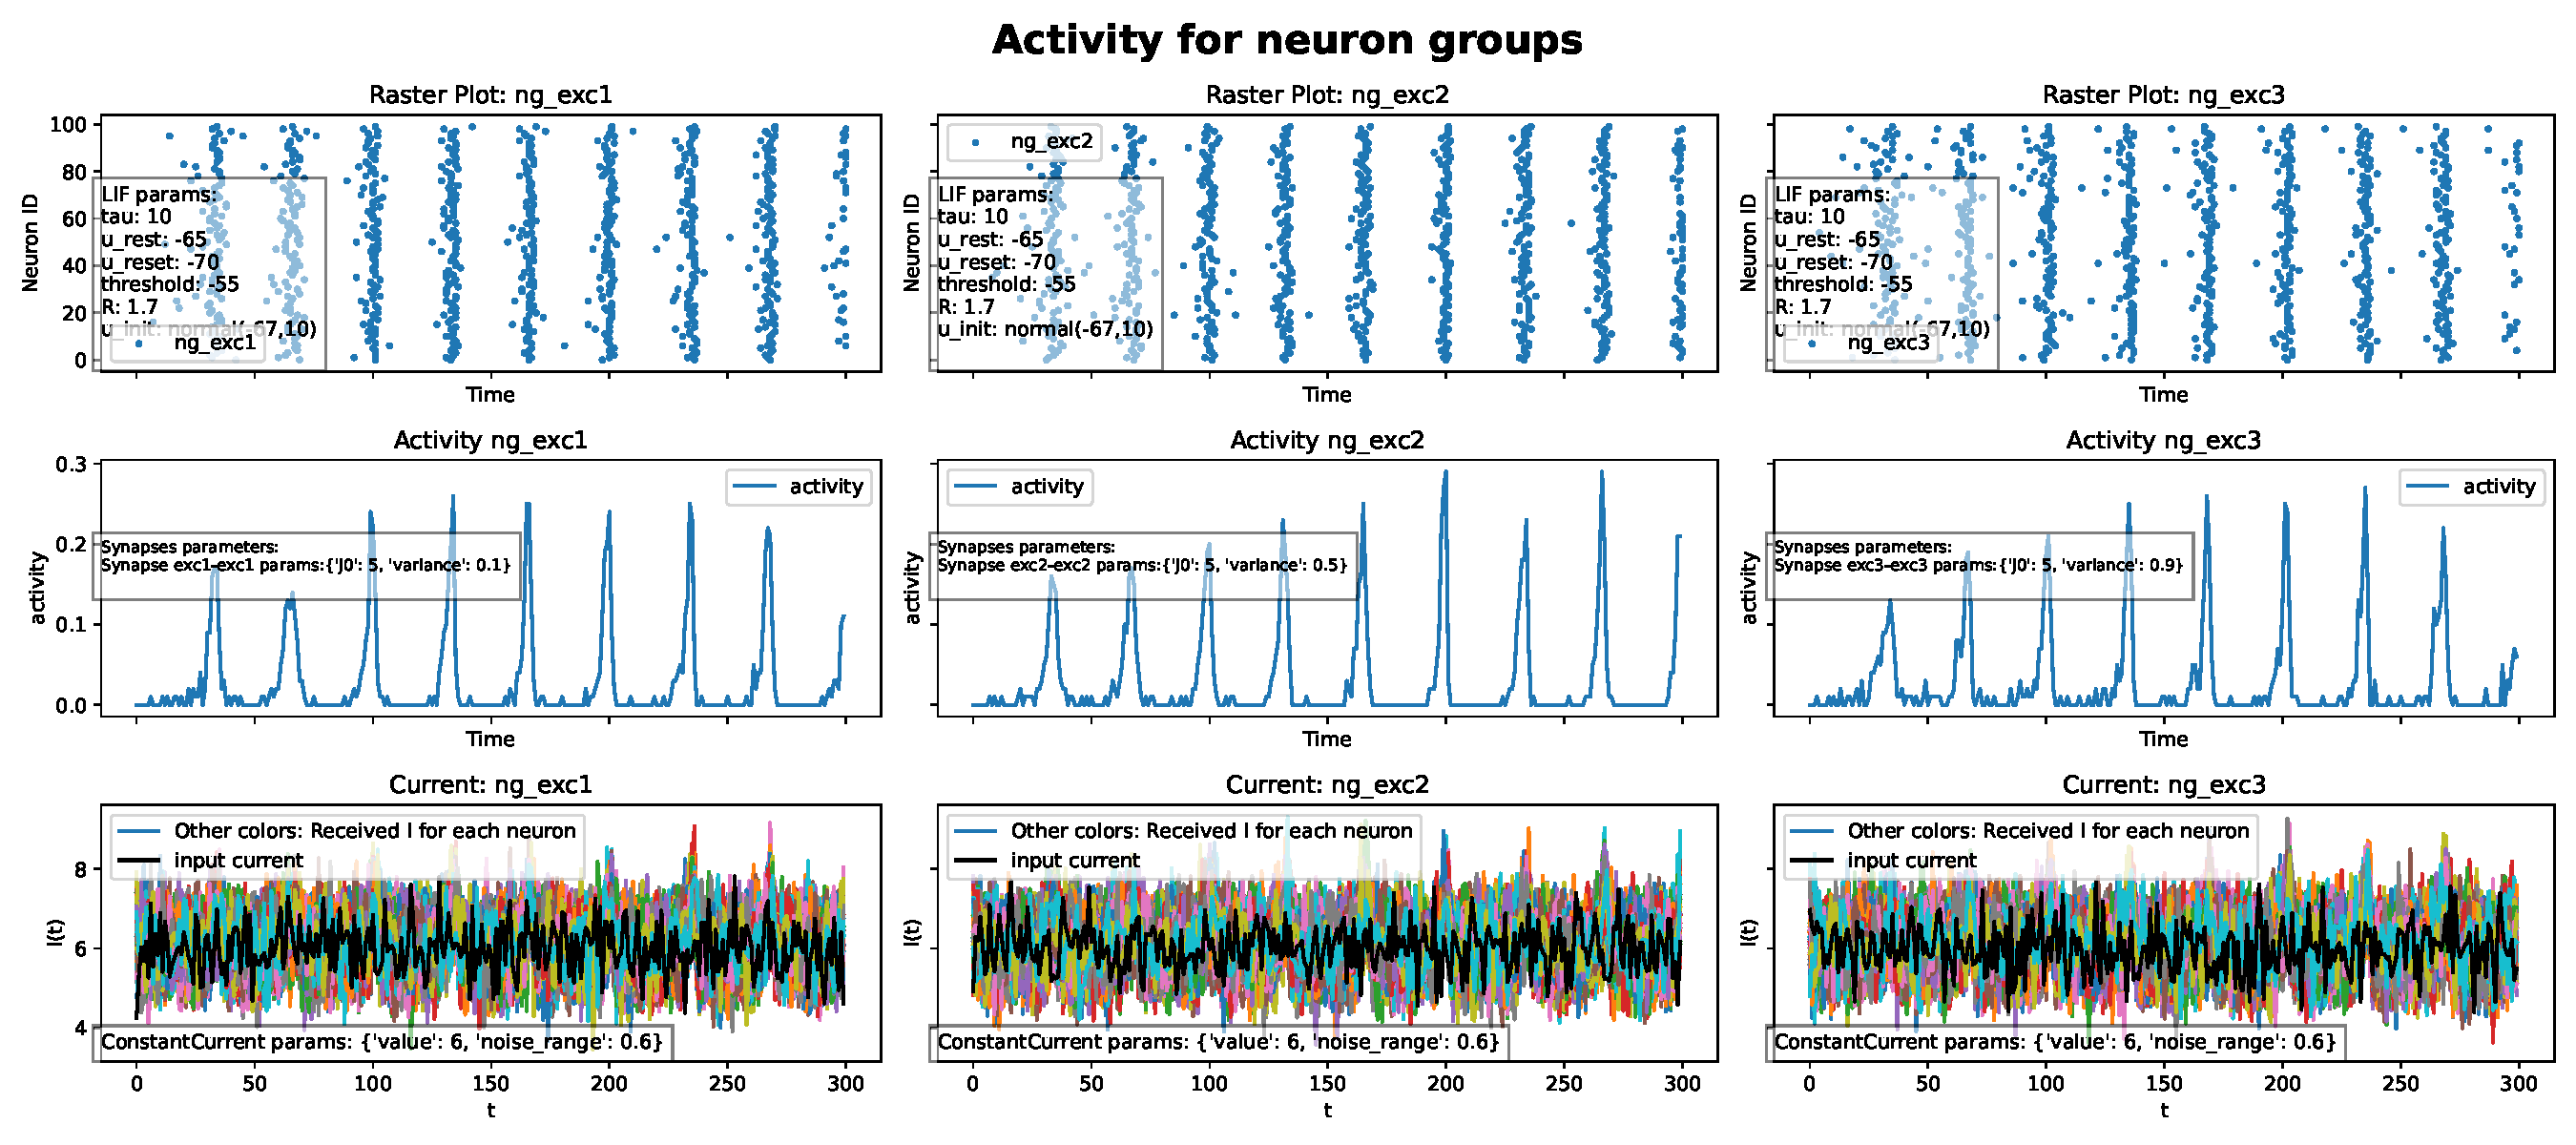
\includegraphics[width=0.9\textwidth]{plots/part2-one-ng-full-synapse-diff-variance.pdf} 
                    \caption{رفتار یک جمعیت نورونی با واریانس مختلف و جریان ثابت نویزدار}
                    \label{fig:part2-one-ng-full-synapse-diff-variance}
                \end{figure}

                حال رفتار را با یک جریان تصادفی آزمایش می کنیم. در جریان تصادفی نیز مطابق شکل
                \ref{fig:part2-one-ng-full-synapse-diff-variance-rand-curr}
                دریافت می شود که تغییر واریانس تاثیر چندانی بر روی رفتار جمعیت ندارد. به طور کلی میتوان این نتیجه را گرفت که در الگوی ارتباط کامل با جریان غیر ثابت، به دلیل اینکه همه نورون ها با یکدیگر در ارتباط هستند، افزودن واریانس به وزن ها نمیتواند روی جریان تصادفی تاثیر بگذارد.

                \begin{figure}[!ht]
                    \centering
                    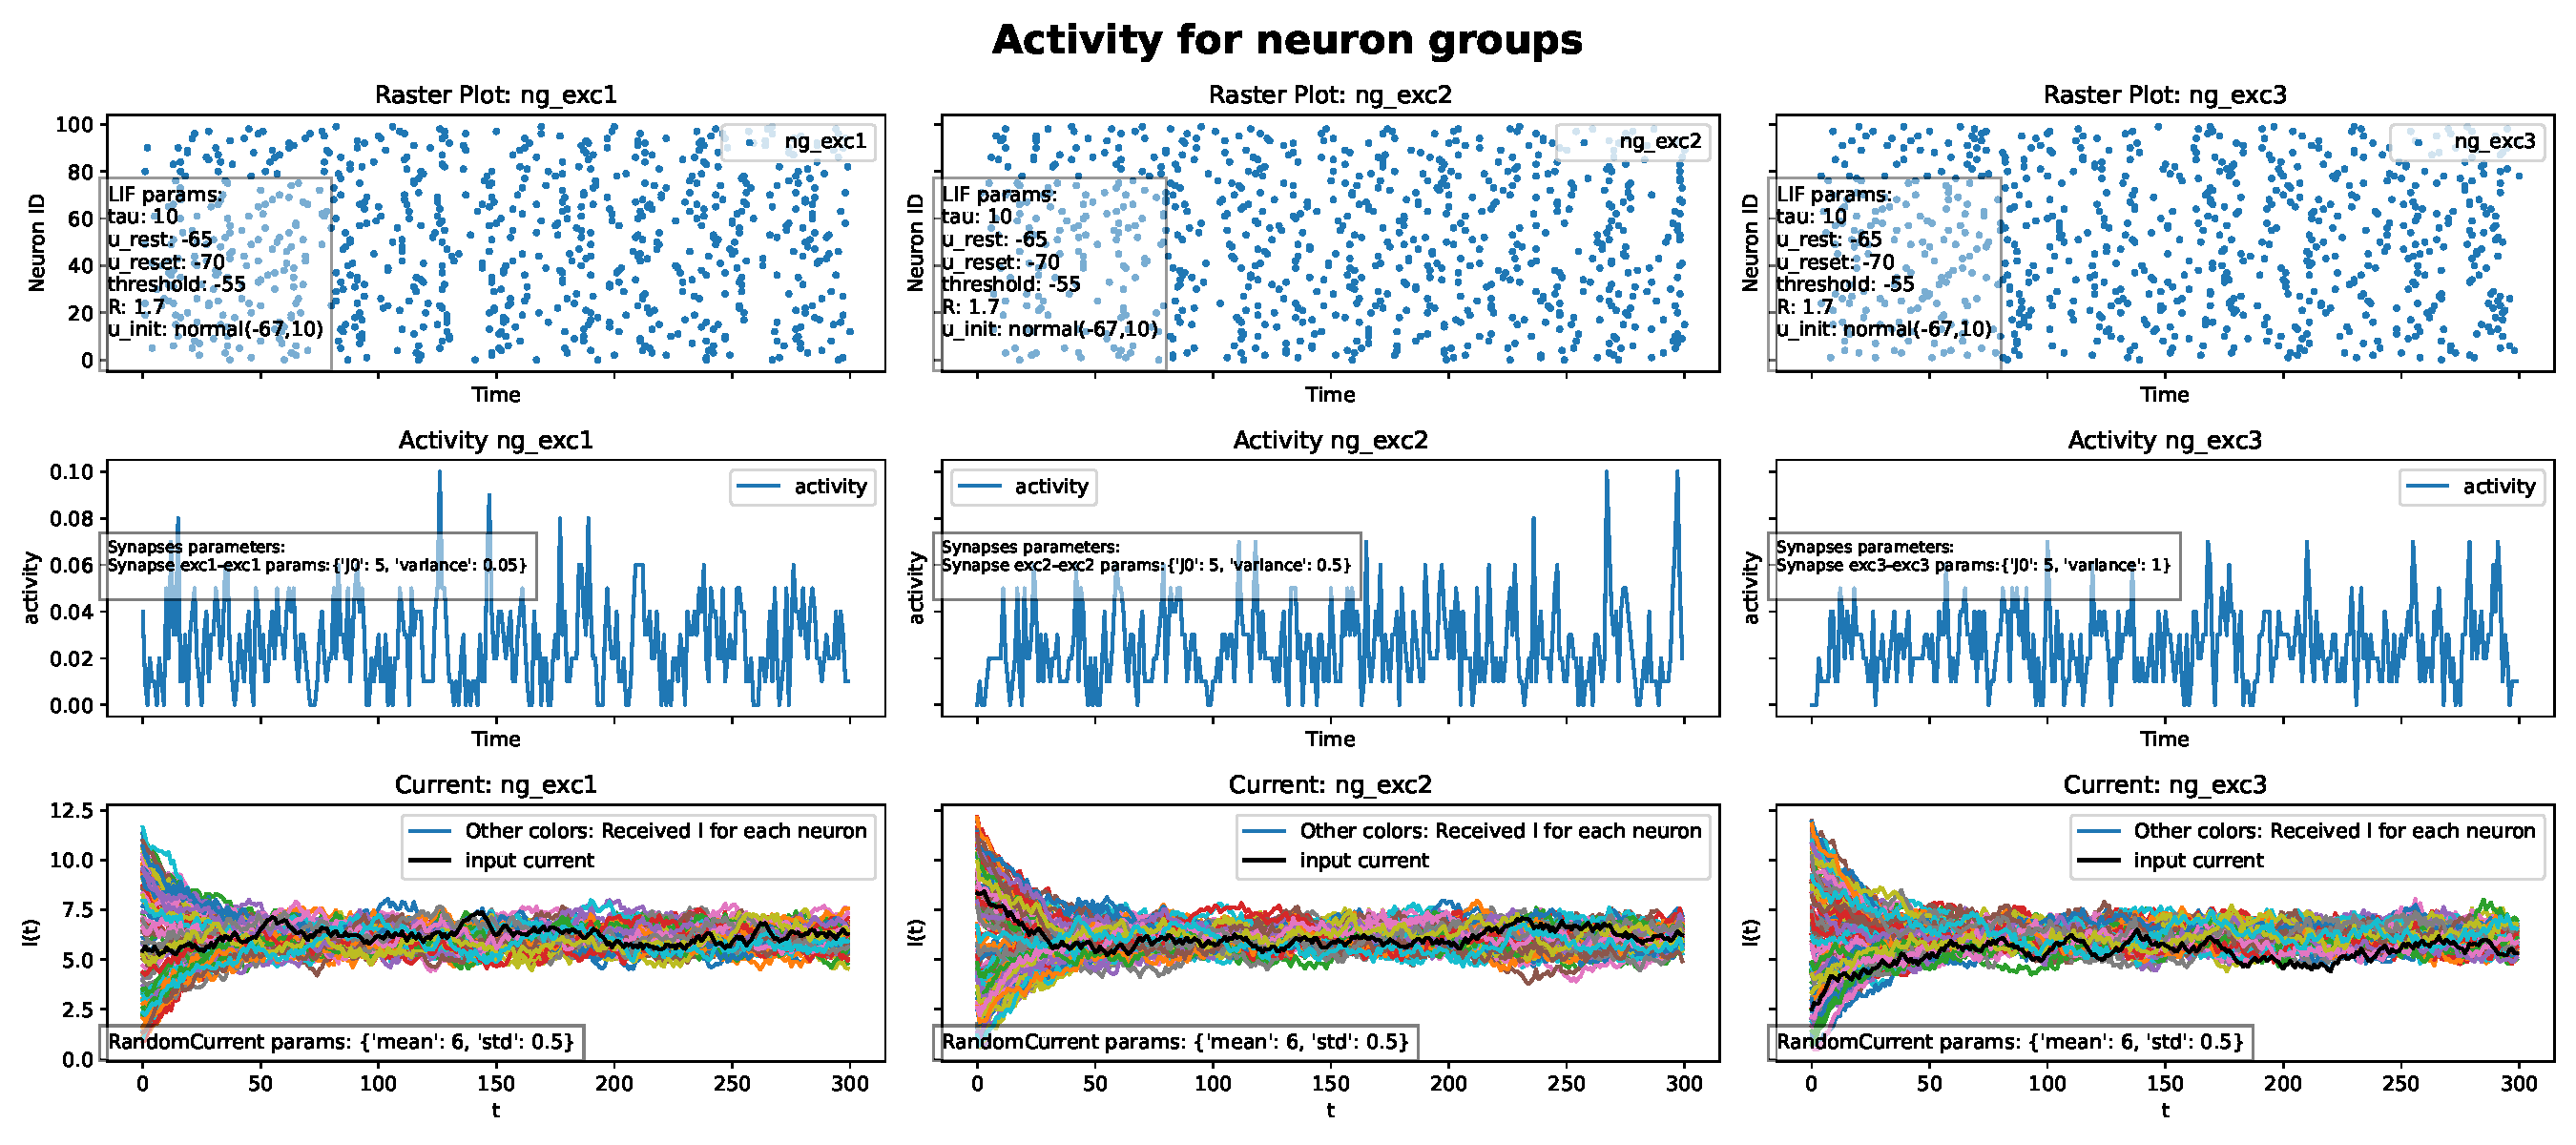
\includegraphics[width=0.9\textwidth]{plots/part2-one-ng-full-synapse-diff-variance-rand-curr.pdf} 
                    \caption{رفتار یک جمعیت نورونی با واریانس مختلف و جریان تصادفی}
                    \label{fig:part2-one-ng-full-synapse-diff-variance-rand-curr}
                \end{figure}

            \paragraph*{اندازه جمعیت}
                خالی از لطف نیست که تاثیر اندازه جمعیت را روی رفتار آن بررسی میکنیم. برای اینکار سه جمعیت نورونی به اندازه های ۵۰، ۱۰۰ و ۲۵۰ را بررسی میکنیم تا ببینیم اندازه چه تاثیری روی رفتار جمعیت دارد. طبق شکل
                \ref{fig:part2-one-ng-full-synapse-diff-size}
                مشاهده می کنیم که اگر مدل نورون ها و جریان را یکی بگیریم، برای جمعیت با اندازه های متفاوت، فعالیت نورونی تغییری نکرده و مستقل از اندازه جمعیت است.
                \begin{figure}[!ht]
                    \centering
                    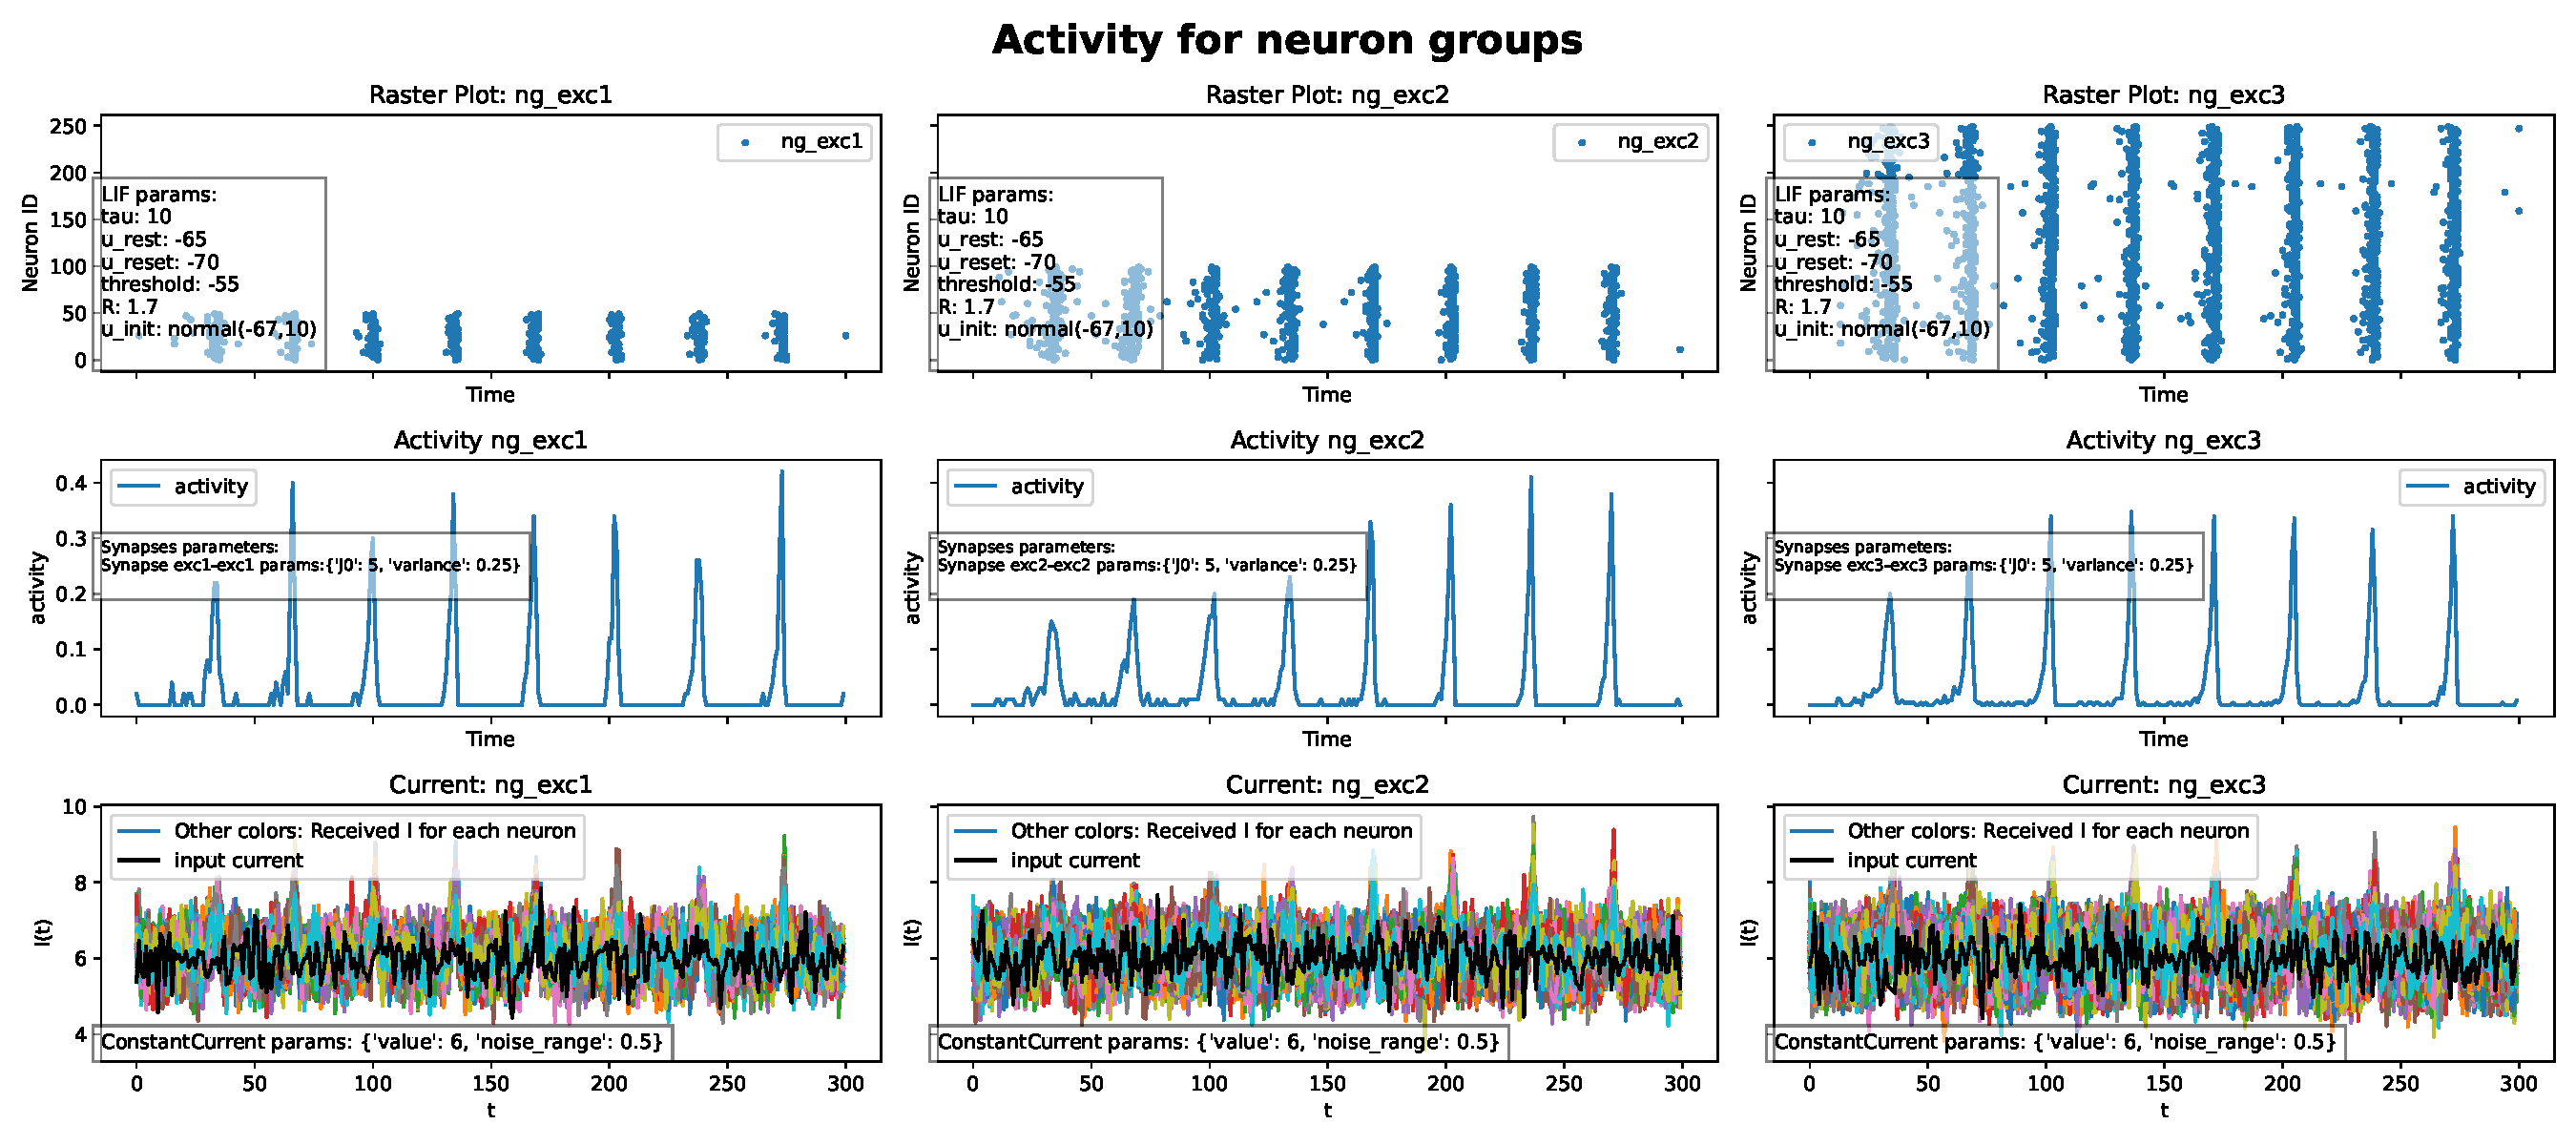
\includegraphics[width=0.9\textwidth]{plots/part2-one-ng-full-synapse-diff-size.pdf} 
                    \caption{رفتار یک جمعیت نورونی با واریانس مختلف و جریان تصادفی}
                    \label{fig:part2-one-ng-full-synapse-diff-size}
                \end{figure}
            \paragraph*{مدل های نورونی}
                در نهایت نیز به سراغ بررسی تاثیر انتخاب مدل نورونی روی رفتار جمعیت میرویم. همانطور که از شکل
                \ref{fig:part2-one-ng-full-synapse-diff-neuron-model}
                پیداست، رفتار مدل نورونی 
                $LIF$ و
                $ELIF$ 
                شبیه یکدیگر است در حالی که در مدل 
                $AELIF$ 
                با گذر زمان، فعالیت نورونی کاهش یافته و به مقدار کمتری همگرا می شود.
                \begin{figure}[!ht]
                    \centering
                    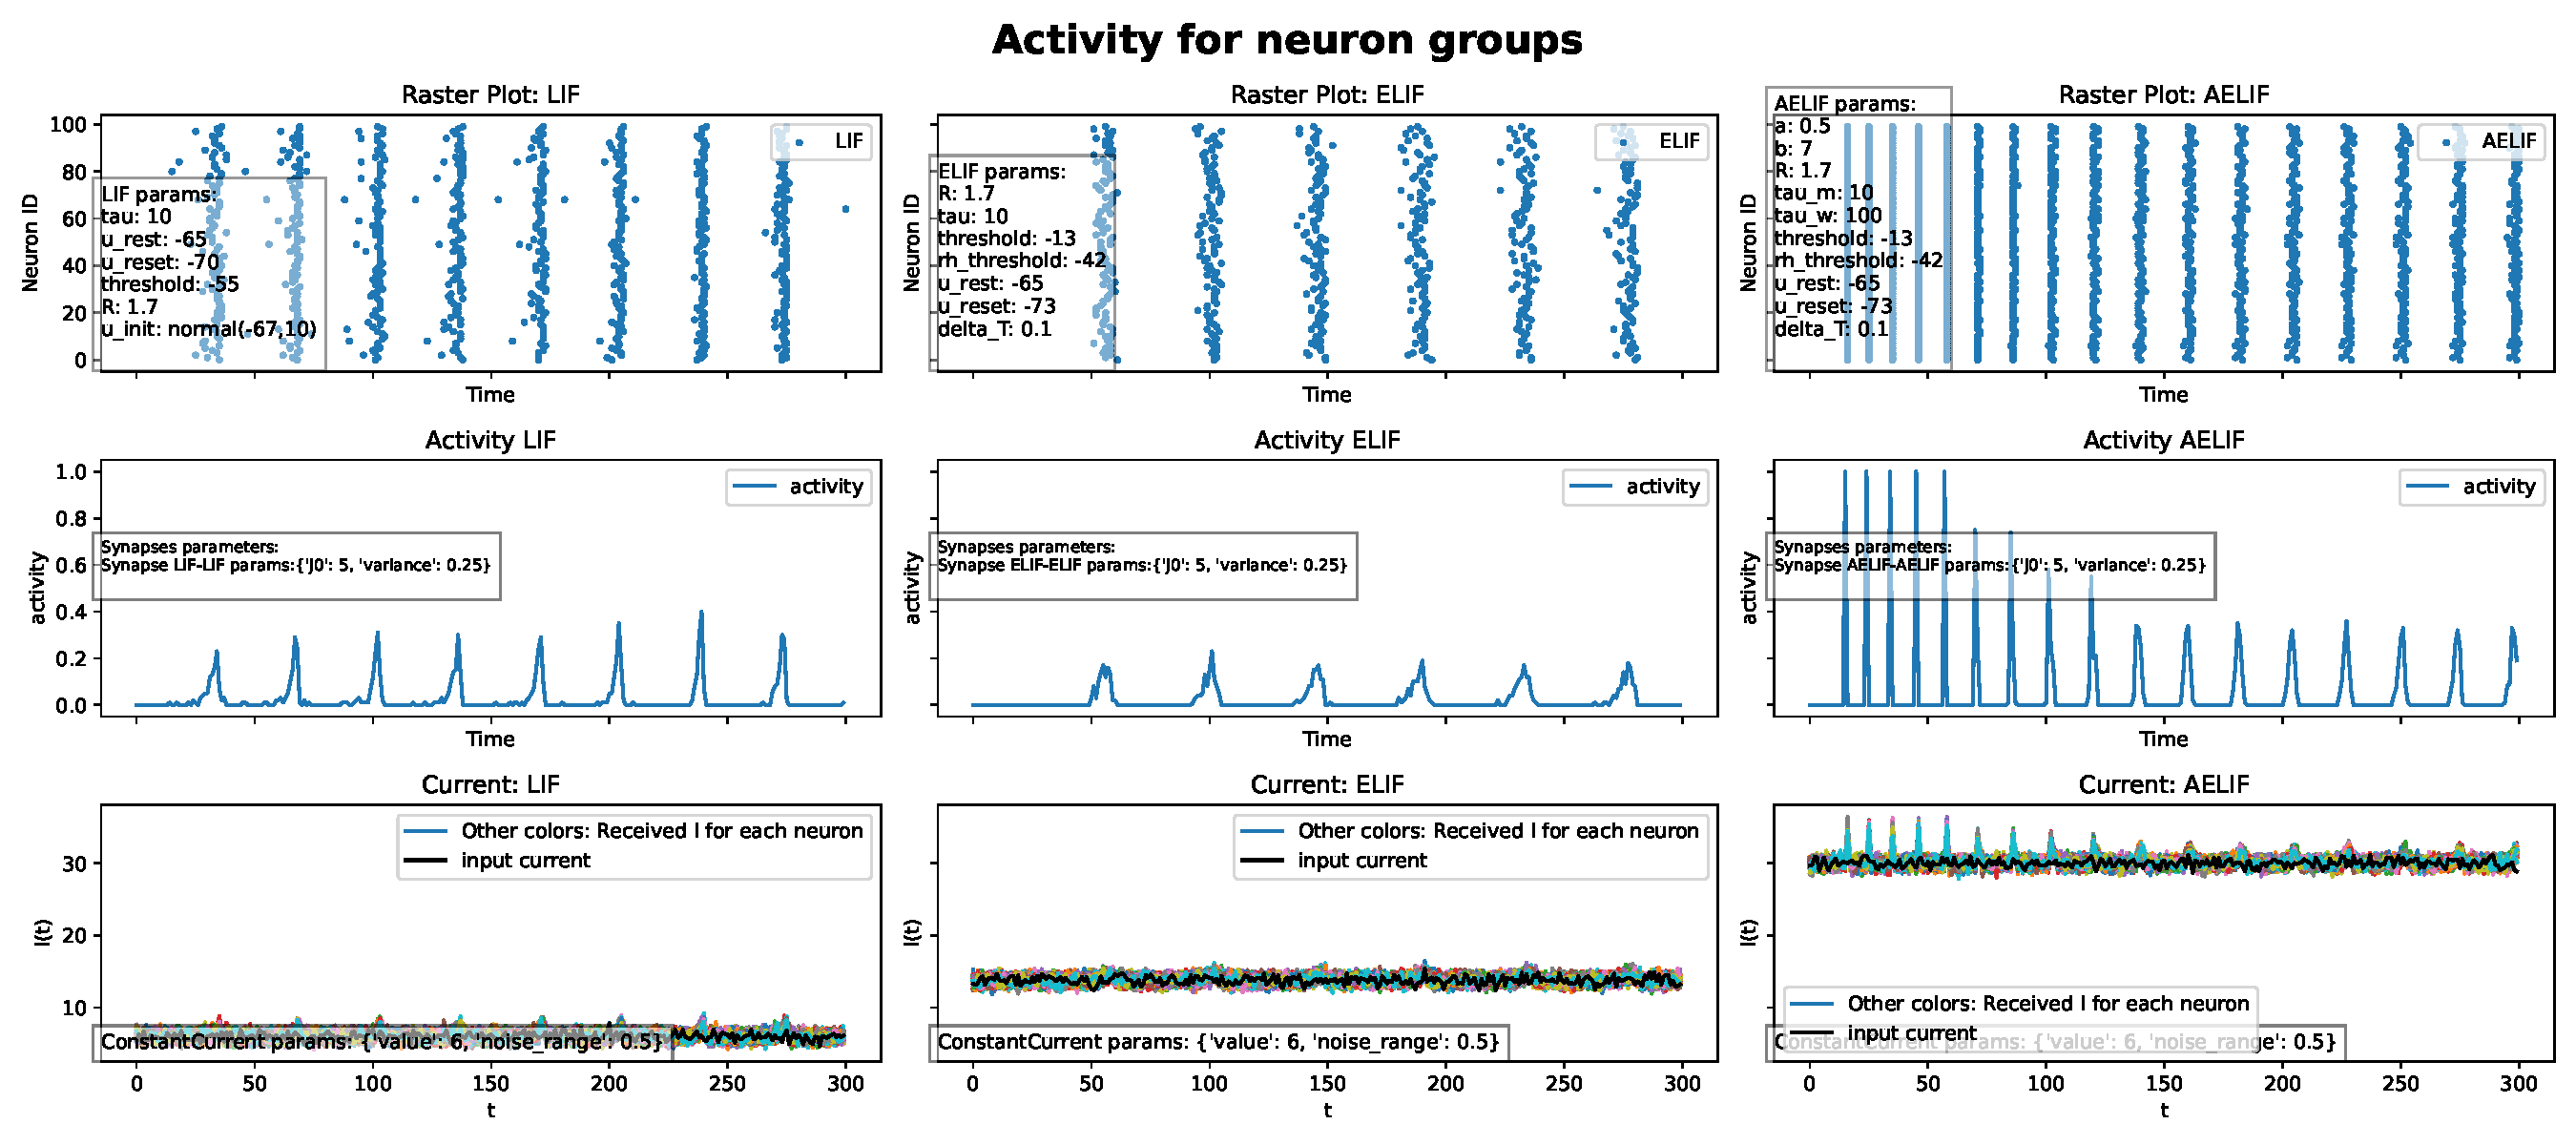
\includegraphics[width=0.9\textwidth]{plots/part2-one-ng-full-synapse-diff-neuron-model.pdf} 
                    \caption{رفتار یک جمعیت نورونی با واریانس مختلف و جریان تصادفی}
                    \label{fig:part2-one-ng-full-synapse-diff-neuron-model}
                \end{figure}
        \subsubsection*{بررسی رفتار دو جمعیت}
            \paragraph*{پارامتر $j_0$}
            حال به بررسی رفتار دو جمعیت که بین آن ها سیناپس قرار دارد می پردازیم. در این بخش   تاثیر دو جمعیت روی یکدیگر را بررسی میکنیم. اولین حالتی که مورد بررسی قرار می دهیم، حالتی است که دو حمعیت تحریکی هستند و فقط به یکدیگر سیناپس دارند و سیناپس داخلی بین نورون های آن ها وجود ندارد.
            در این حالت با نتایجی که تا الآن بدست آورده ایم انتظار داریم که فعالیت دو نورون شبیه یک دیگر باشند که شکل
            \ref{fig:part2-two-ng-full-synapse-noise-curr}
            نیز این موضوع را تایید میکند. جریان تصادفی نیز رفتار مشابهی از خود نشان می دهد. 
            (شکل \ref{part2-two-ng-full-synapse-rand-curr})
            \begin{figure}[!ht]
                \centering
                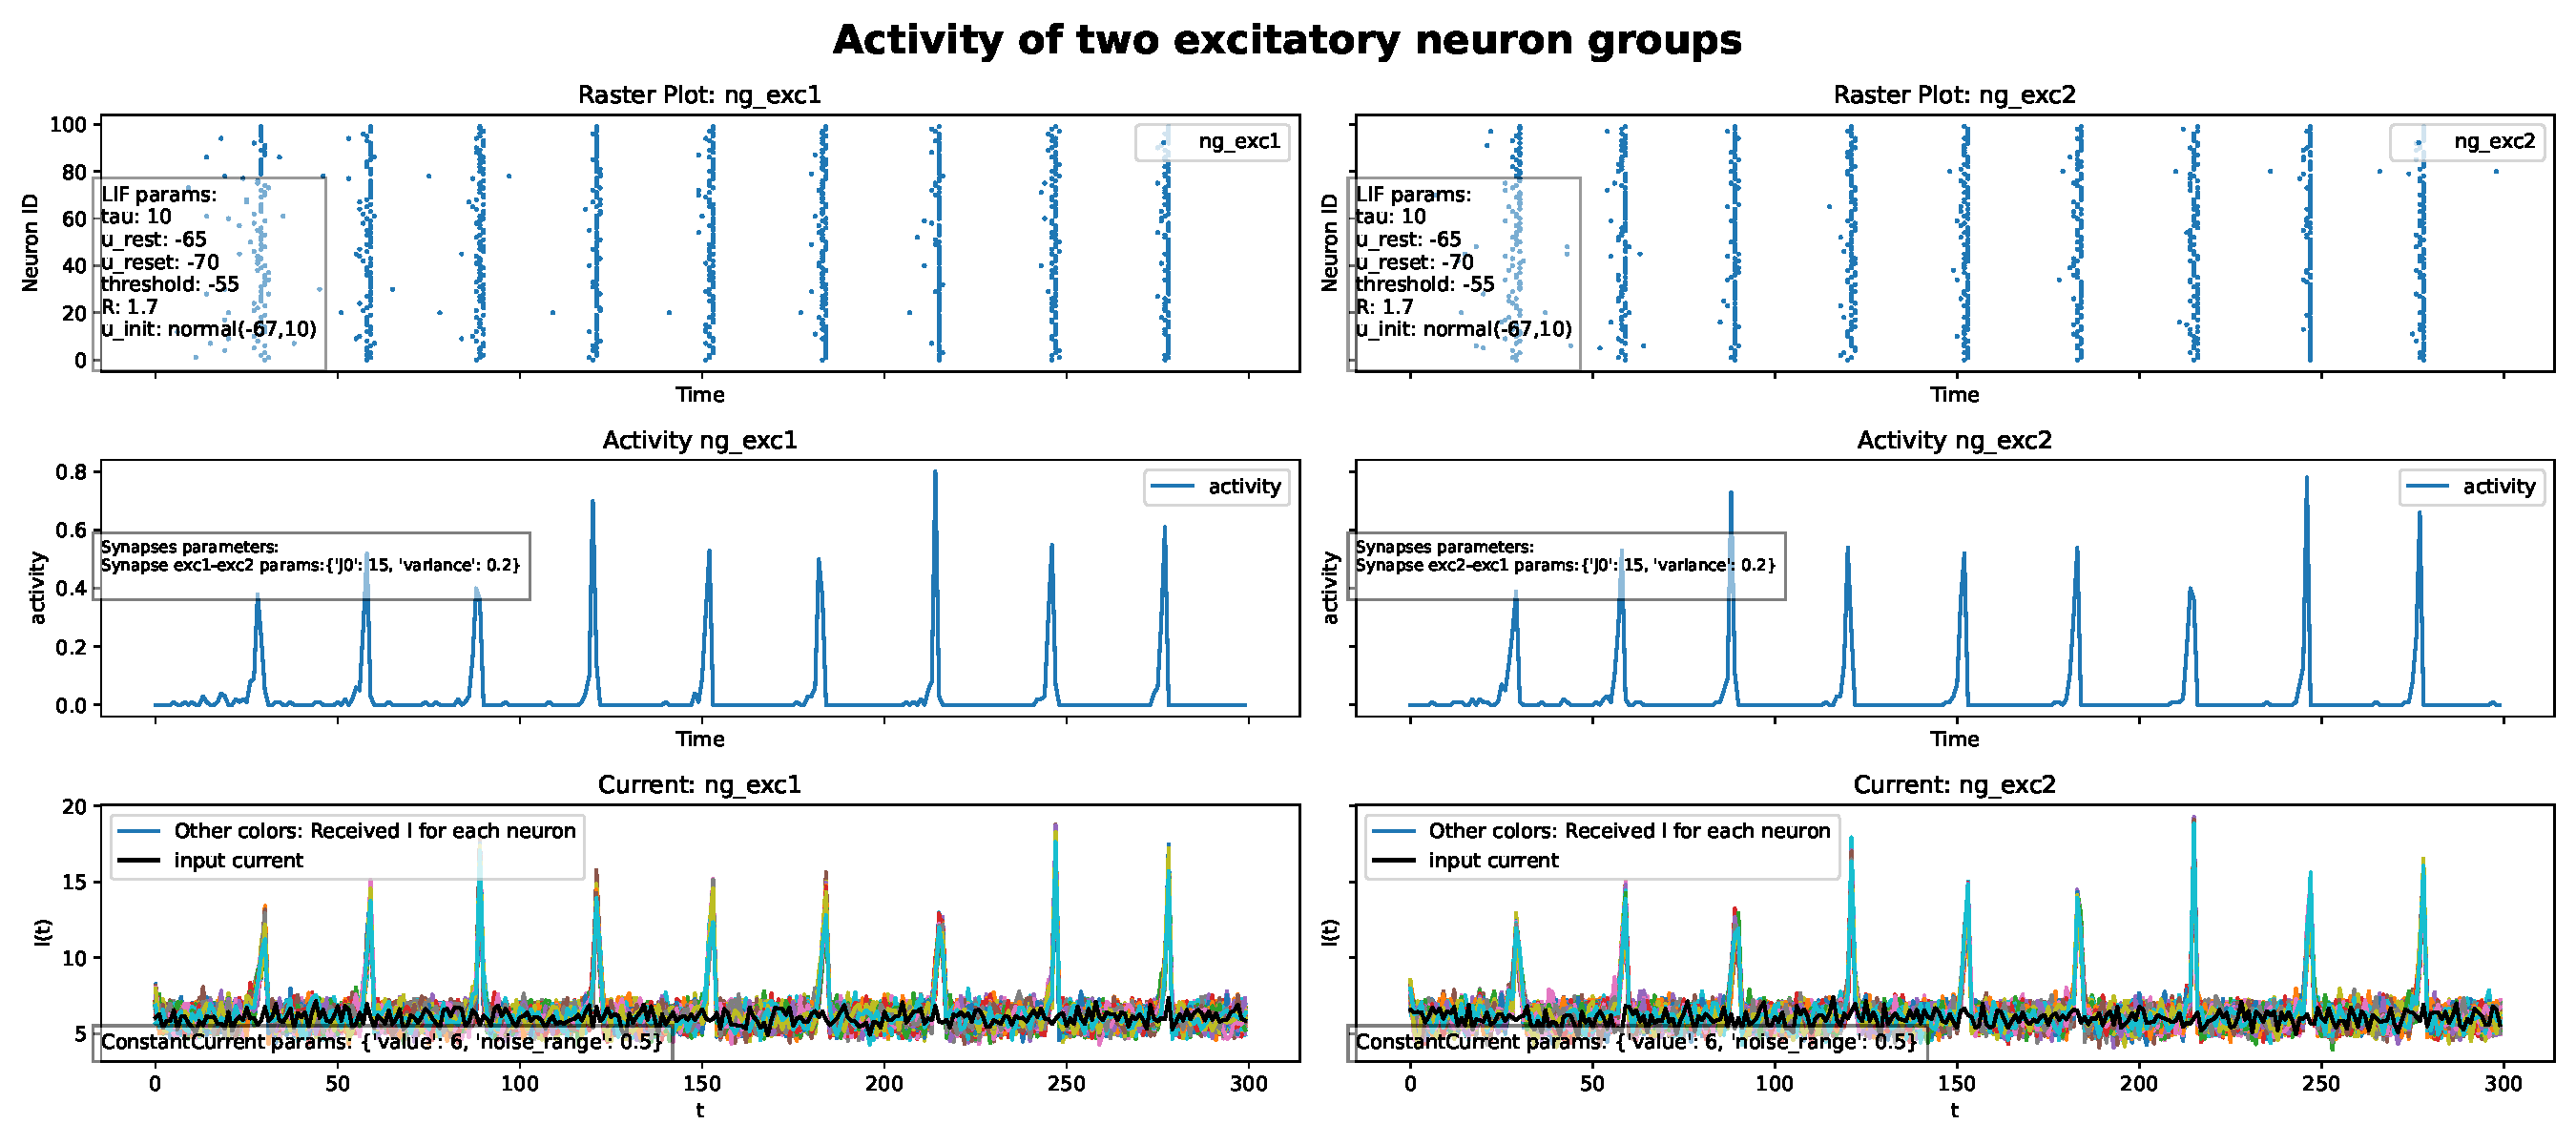
\includegraphics[width=0.9\textwidth]{plots/part2-two-ng-full-synapse-noise-curr.pdf} 
                \caption{رفتار دو جمعیت نورونی با دو سیناپس و جریان ثابت نویزی}
                \label{fig:part2-two-ng-full-synapse-noise-curr}
            \end{figure}
            \begin{figure}[!ht]
                \centering
                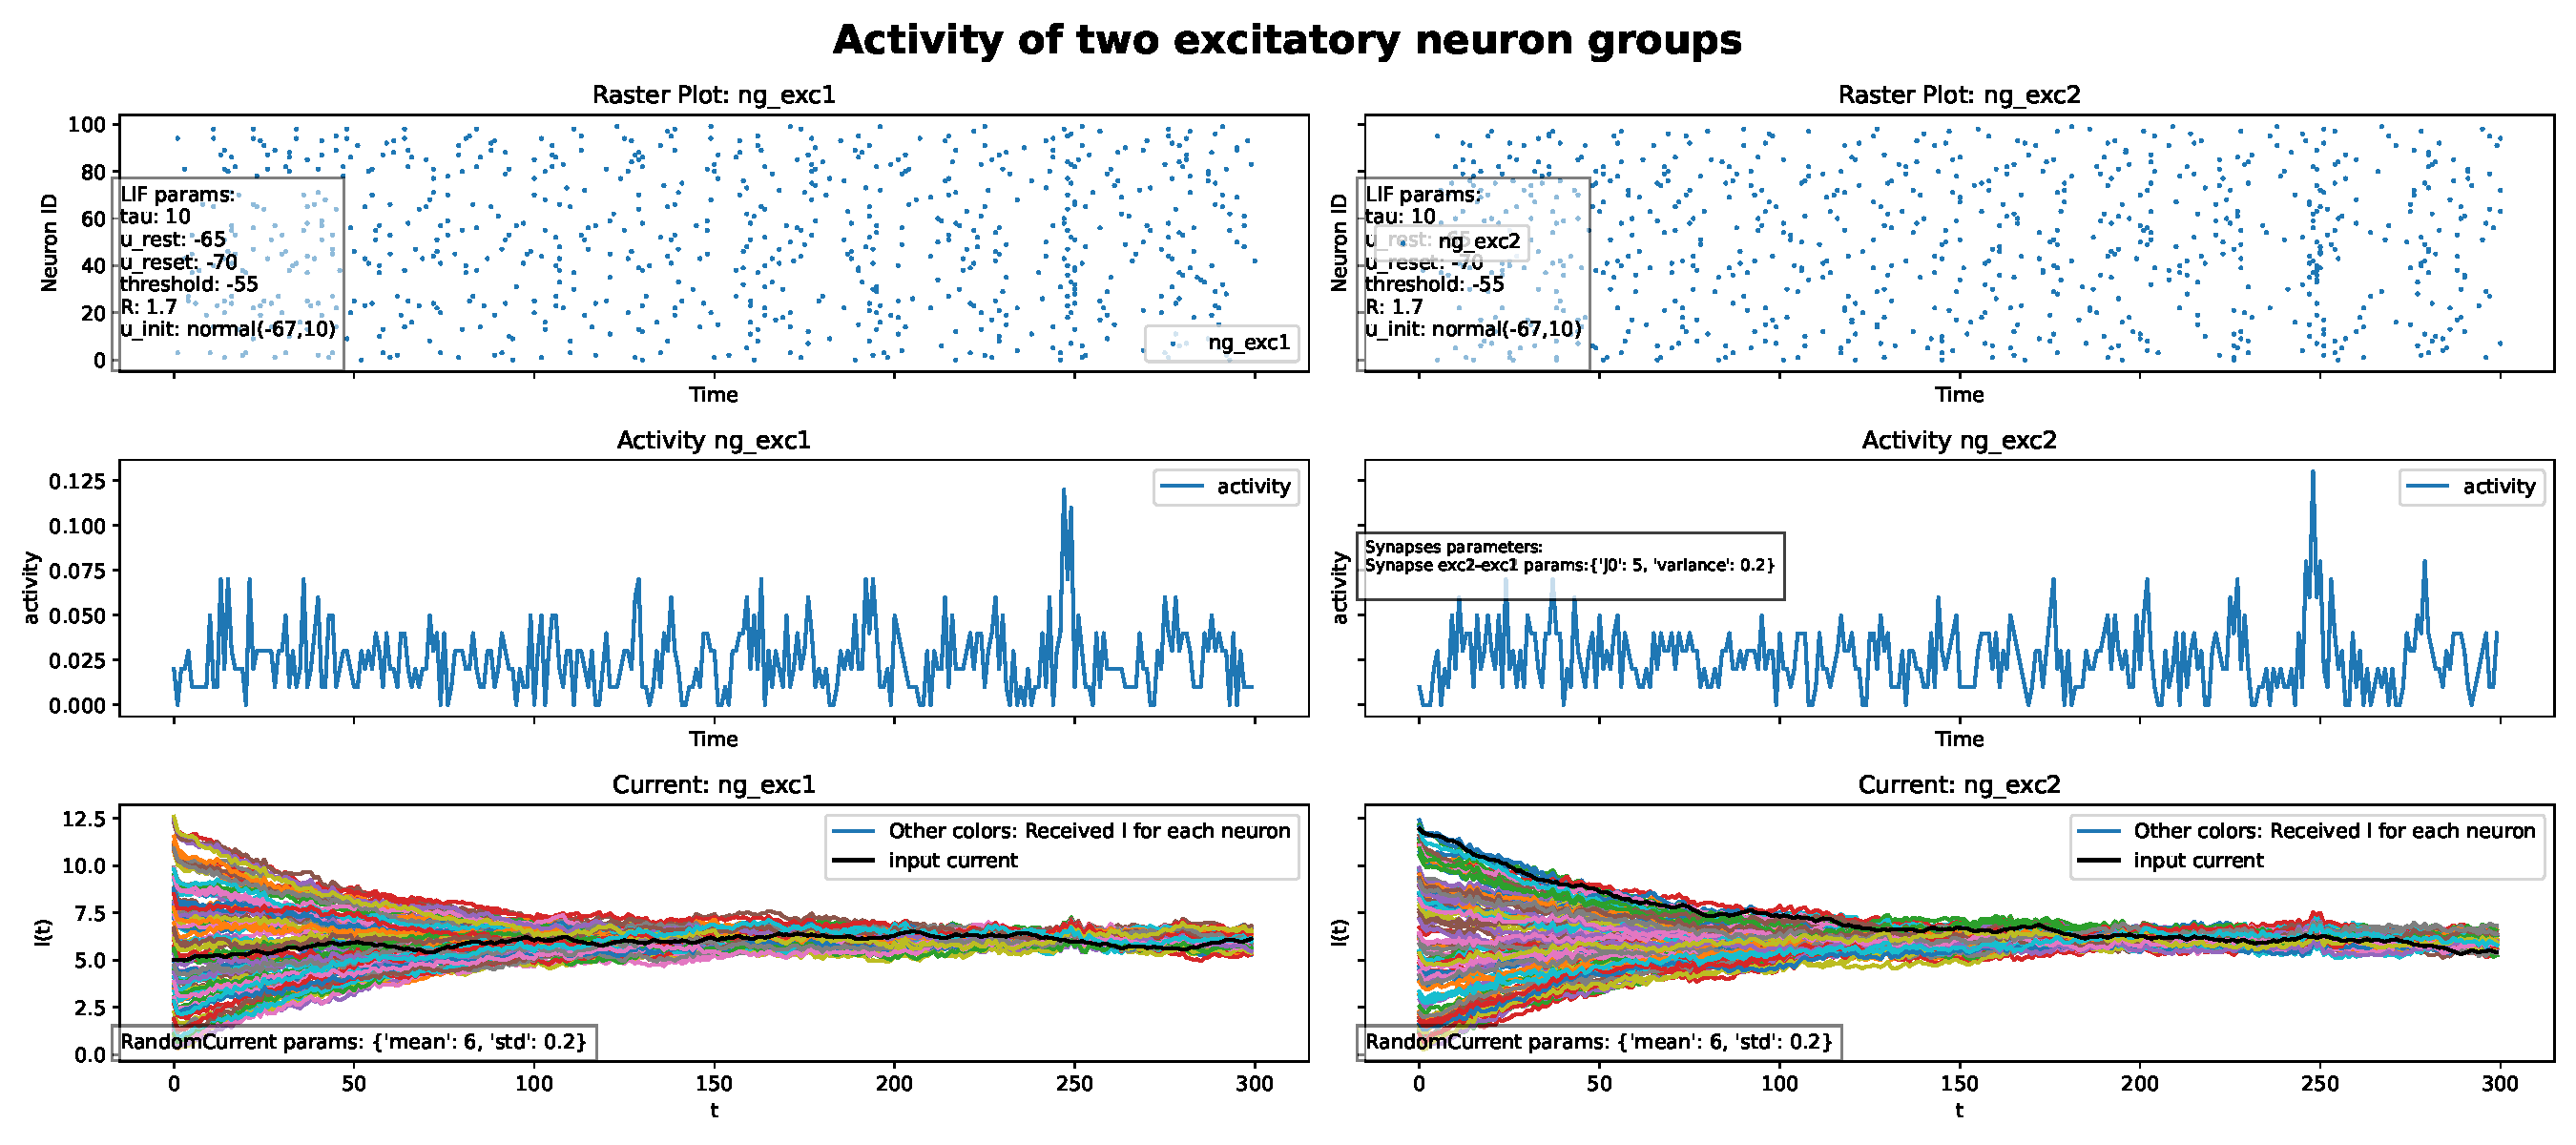
\includegraphics[width=0.9\textwidth]{plots/part2-two-ng-full-synapse-rand-curr.pdf} 
                \caption{رفتار دو جمعیت نورونی با دو سیناپس و جریان تصادفی}
                \label{fig:part2-two-ng-full-synapse-rand-curr}
            \end{figure}

            رفتار جالب دیگری که جریان تصادفی دارد، این است که در ابتدا پراکندگی زمان ضربه زدن نورون ها بسیار زیاد است و الگوی خای ندارد، و همچنین فعالیت نورونی کم است، اما همانطور که از نمودار پیداست، این پراکندگی رفته رفته کمتر شده و فعالیت نورونی نیز بیشتر می شود. این اتفاق تحت تاثیر این موضوع است که به دلیل وجود سنیاپس بین دو جمعیت که به صورت رفت و برگشتی است، به گونه ای عمل کرده که هر نورون از تمام نورون های جمعیت دیگر جریان دریافت میکند و درنتیجه جریان دریافتی به نورون زیاد می شود و این جریان زیاد باعث می شود تا پس از مدتی زمان ضربه زدن نورون ها به یکدیگر نزدیک شود.

            حال اگر مقدار 
            $j_0$ 
            را در هر ۲ سیناپس کاهش دهیم چه اتفاقی می افتد؟ شکل 
            \ref{part2-two-ng-full-synapse-low-j-rand-curr}
            به این سوال پاسخ می دهد و بیان می کند که کاهش مقدار 
            $j_0$ 
            باعث می شود تا جریان سیناپسی نتواند آنقدر زیاد شود که در زمان قبلی پراکندگی فعالیت نورون ها را کمتر کند و فعالیت جمعیت به صورت یک نمودار تصادفی با مقدار کم باقی می ماند.
            \begin{figure}[!ht]
                \centering
                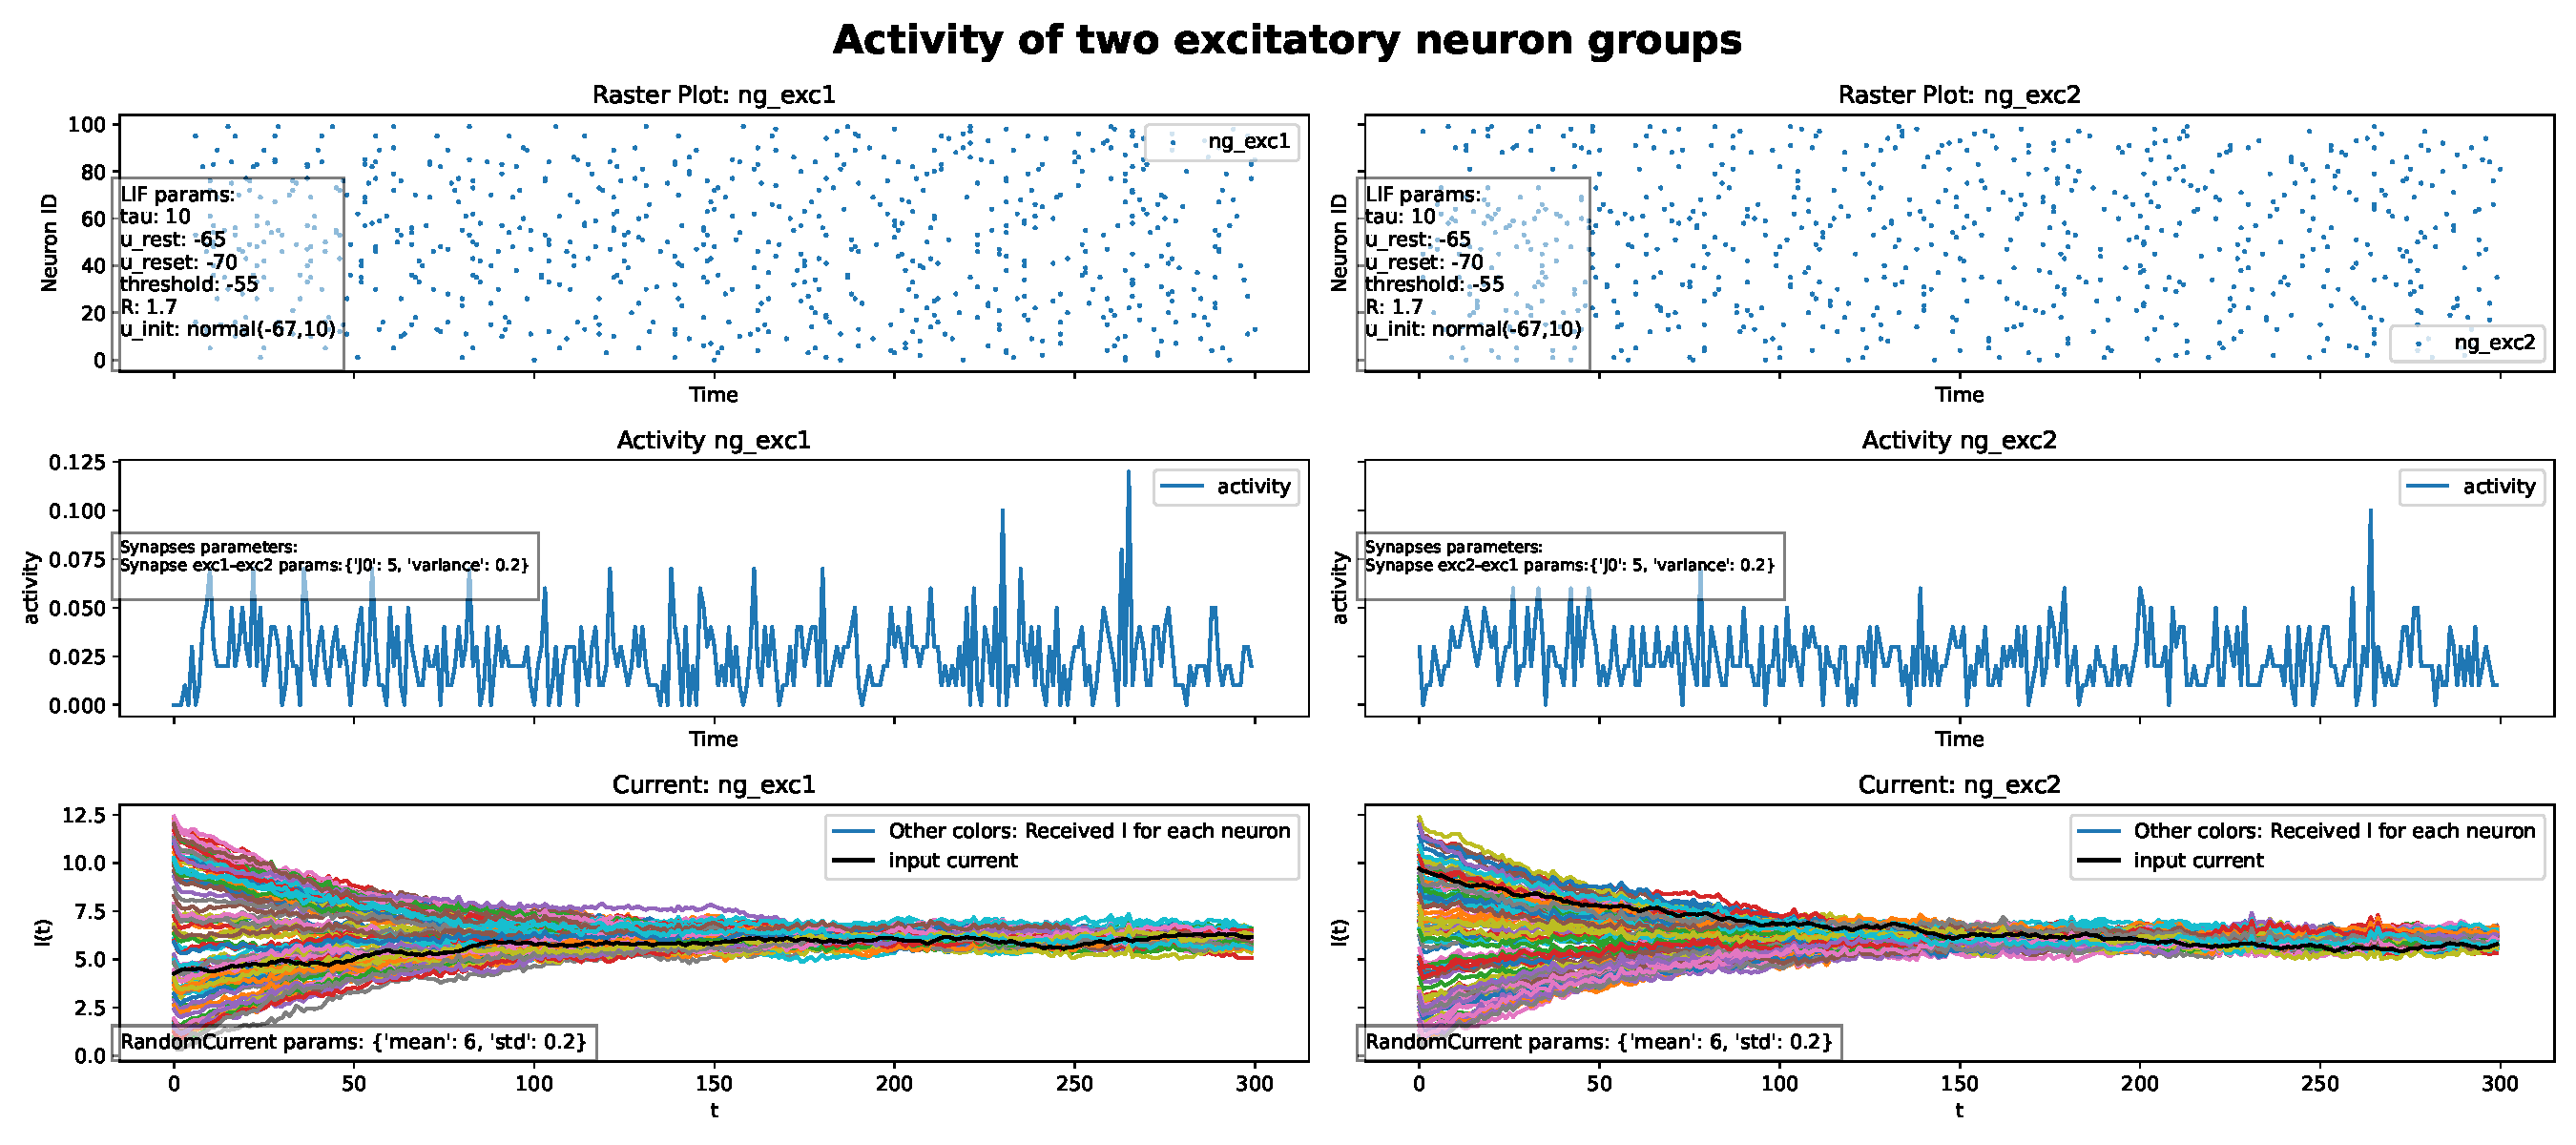
\includegraphics[width=0.9\textwidth]{plots/part2-two-ng-full-synapse-low-j-rand-curr.pdf} 
                \caption{رفتار دو جمعیت نورونی با دو سیناپس و جریان تصادفی و $j_0$ کم}
                \label{fig:part2-two-ng-full-synapse-low-j-rand-curr}
            \end{figure}

            حال مقدار وزن های سیناپس بین جمعیت ۱ به جمعیت ۲ را افزایش میدهیم تا ببینیم با 
            $j_0$
            متفاوت رفتار آن ها چه تغییری میکند. طبق شکل 
            \ref{fig:part2-two-ng-full-synapse-diff-j-rand-curr}
            مشاهده میکنیم که فعالیت هر دو جمعیت بیشتر شده ولی جمعیت ۲ در کل فعالیت بیشتری دارد. مشابه این رفتار را در بخش اول دیدیم، هنگامی که تنها یک سیناپس از جمعیتی به جمعیت دیگر داشتیم و جمعیت پس سیناپسی فعالیت بیشتری داشت. در اینجا نیز گویا همین اتفاق می افتد. بیشتر شدن وزن های سیناپس ۱به۲ باعث می شود که جمعیت ۲ بیشتر ضربه بزند و درنتیجه فعالیت آن بیشتر شود، این بیشتر شدن فعالیت خود باعث می شود که جریان سیناپسی 
            ۲ به ۱
            نیز بیشتر شده و فعالیت جمعیت ۱ نیز بیشتر شود. اما در کل از آنجا که وزن های سیناپسی جمعیت ۱ به ۲ بیشتر است، فعالیت جمعیت ۲ بیشتر از ۱ میماند.
            \begin{figure}[!ht]
                \centering
                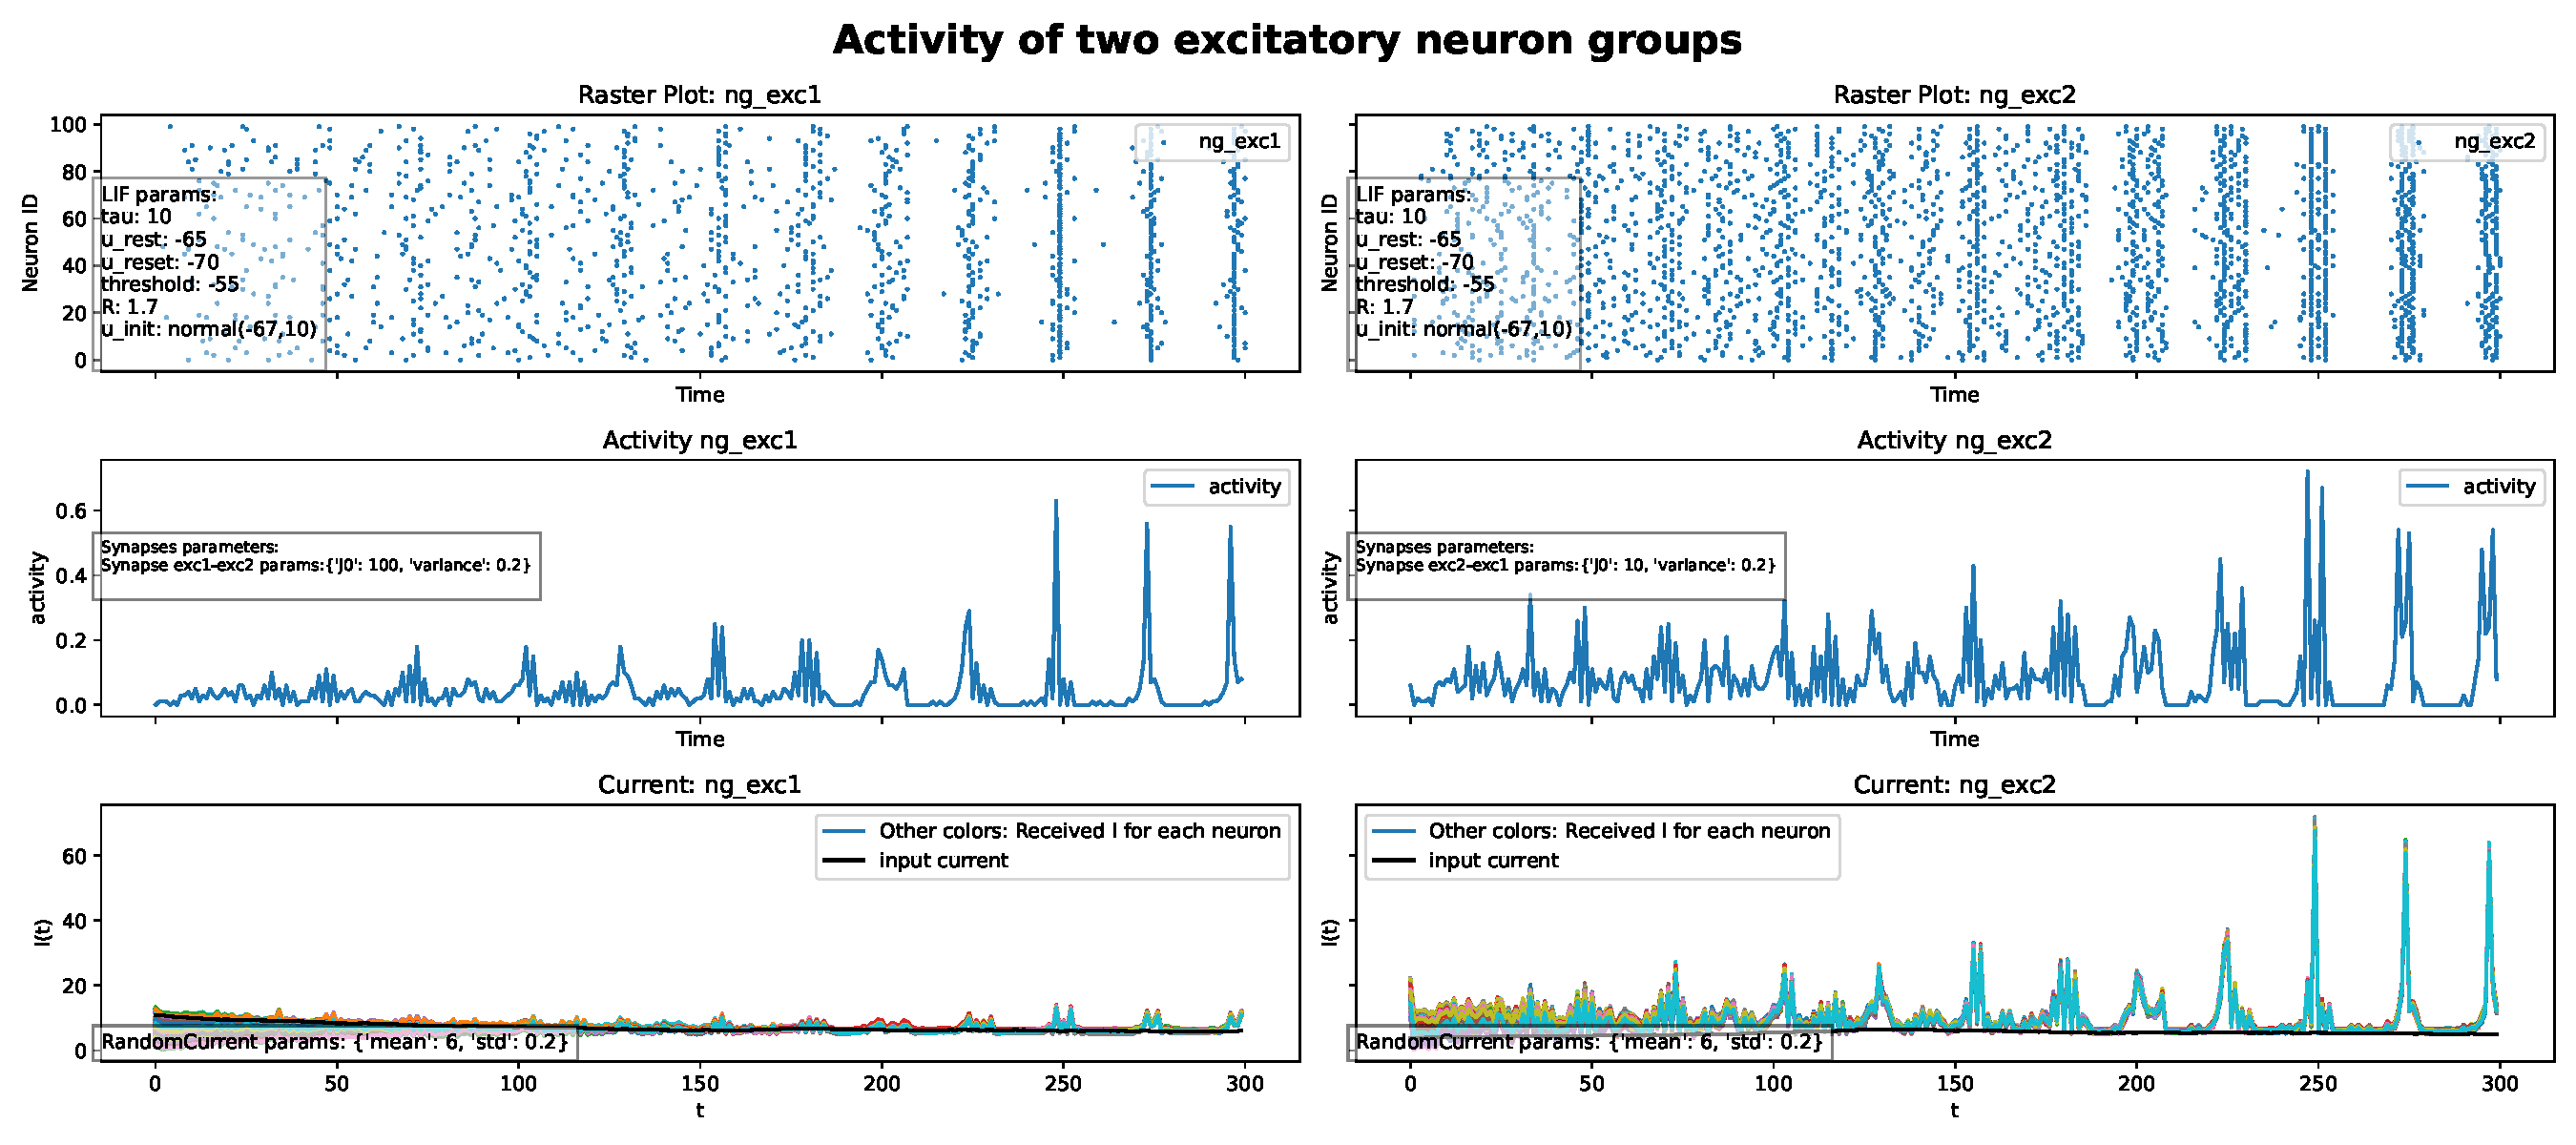
\includegraphics[width=0.9\textwidth]{plots/part2-two-ng-full-synapse-diff-j-rand-curr.pdf} 
                \caption{رفتار دو جمعیت نورونی با دو سیناپس و جریان تصادفی و $j_0$ متفاوت}
                \label{fig:part2-two-ng-full-synapse-diff-j-rand-curr}
            \end{figure}
        \paragraph*{پارامتر واریانس}
            حال با وزن های برابر با شکل 
            \ref{fig:part2-two-ng-full-synapse-noise-curr}
            مقادیر واریانس را افزایش داده و آن را تحلیل میکنیم.
            همانطور که در شکل 
            \ref{fig:part2-two-ng-full-synapse-high-variance-noise-curr} و \ref{fig:part2-two-ng-full-synapse-high-variance-rand-curr}
            مشاهده می شود، افزایش واریانس به علت مشابهی که قبل تر نتیجه گرفته شد، تغییر چندانی در رفتار نورون با جریان های متفاوت ایجاد نمی کند.
            \begin{figure}[!ht]
                \centering
                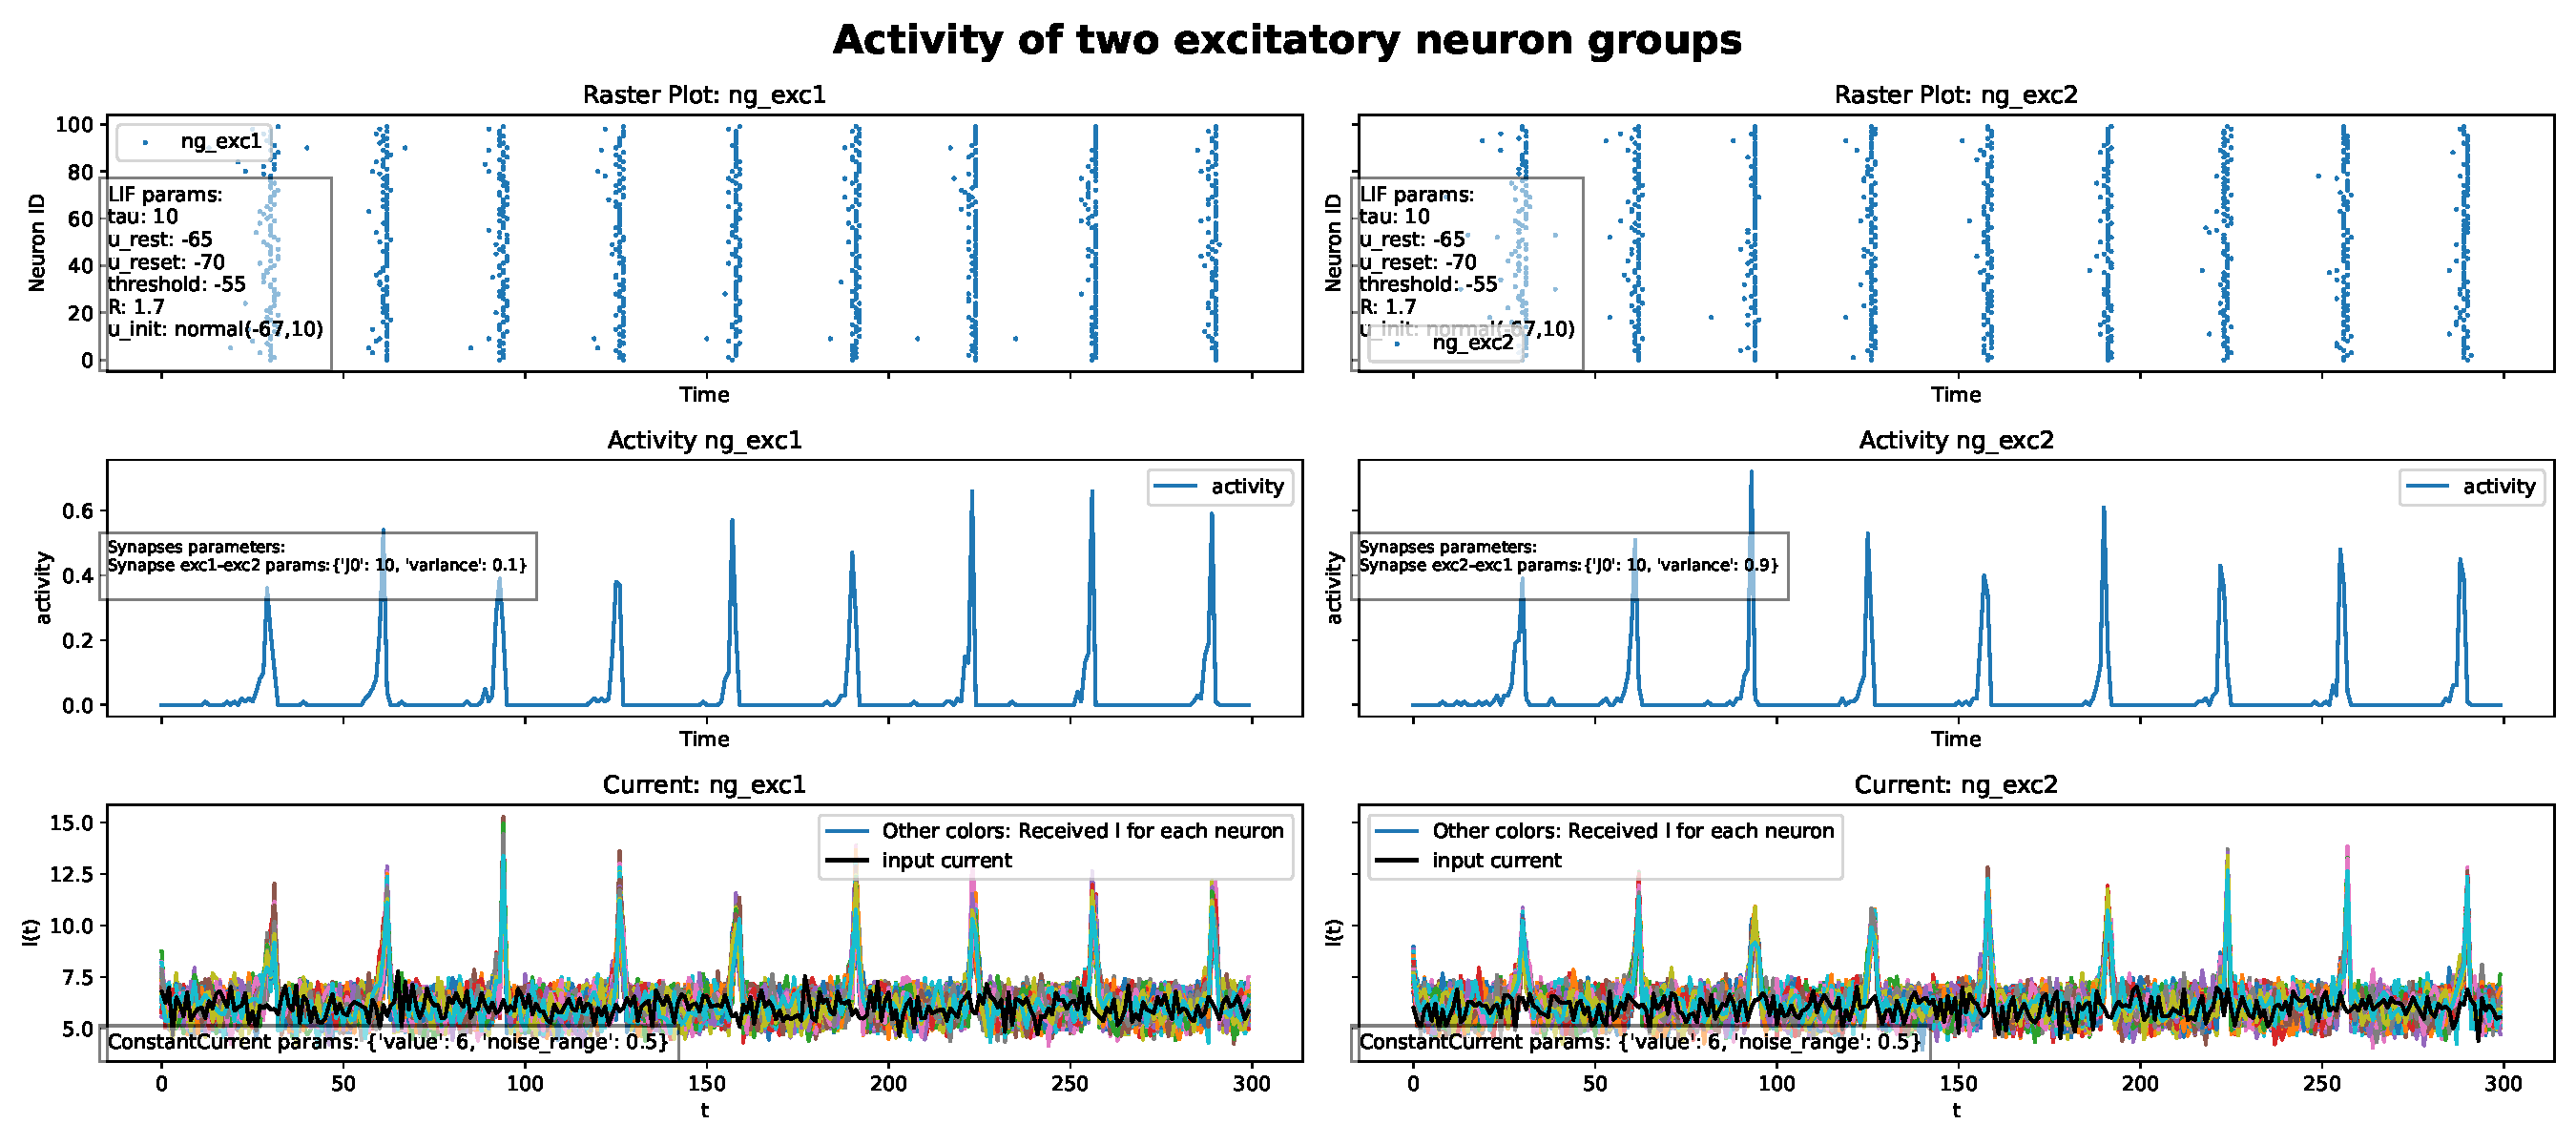
\includegraphics[width=0.9\textwidth]{plots/part2-two-ng-full-synapse-diff-variance-noise-curr.pdf} 
                \caption{رفتار دو جمعیت نورونی با دو سیناپس و جریان نویزی و واریانس زیاد}
                \label{fig:part2-two-ng-full-synapse-high-variance-noise-curr}
            \end{figure}
            \begin{figure}[!ht]
                \centering
                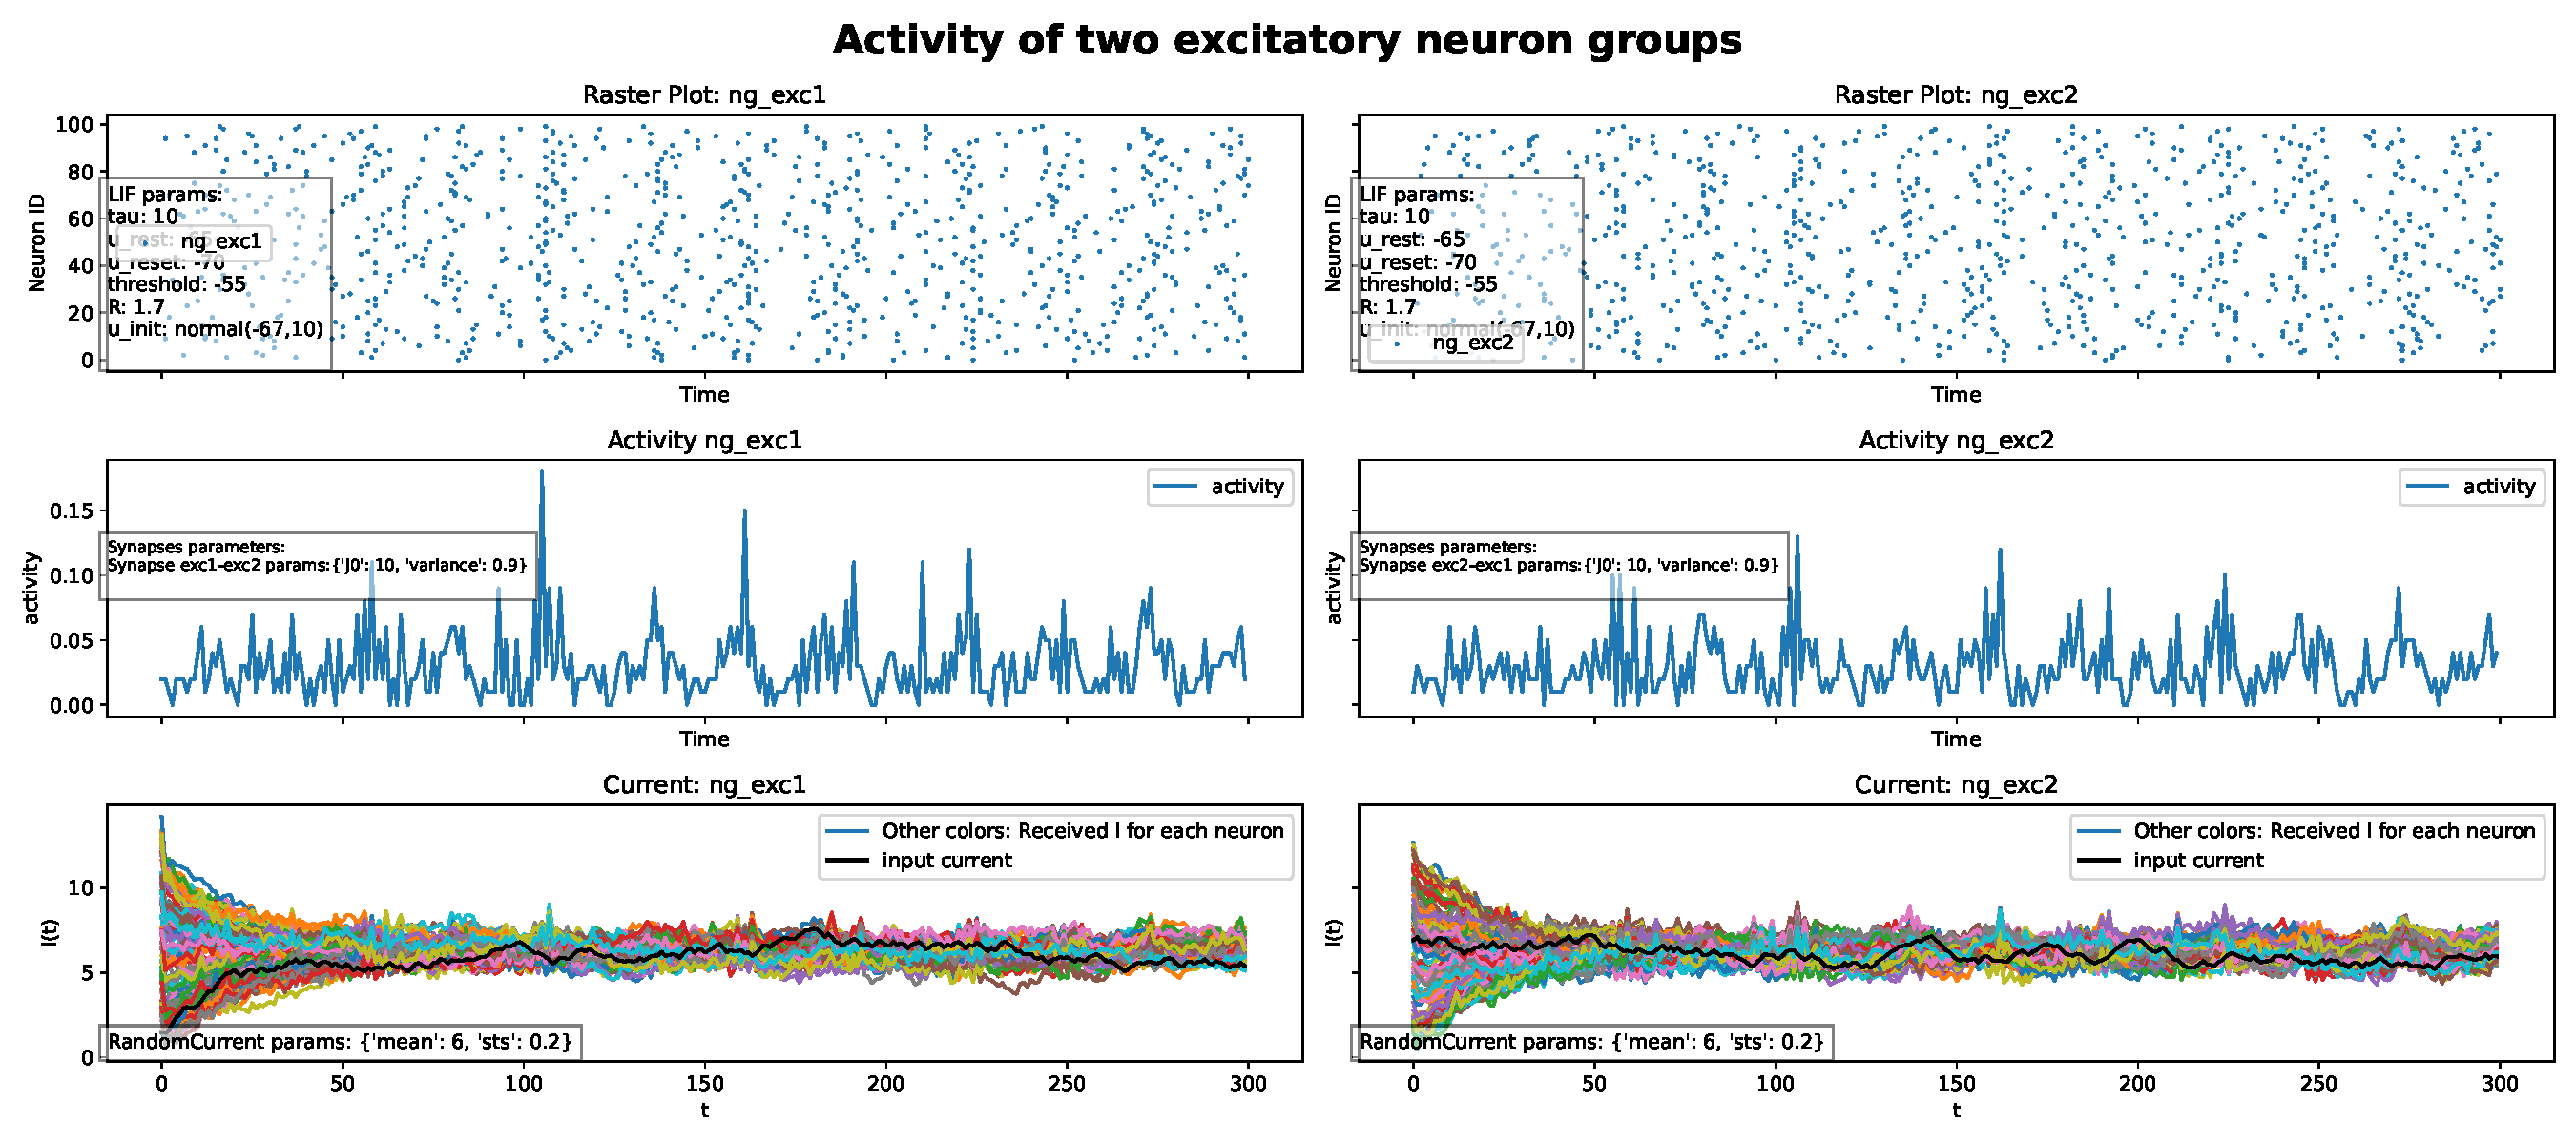
\includegraphics[width=0.9\textwidth]{plots/part2-two-ng-full-synapse-diff-variance-rand-curr.pdf} 
                \caption{رفتار دو جمعیت نورونی با دو سیناپس و جریان نویزی و واریانس زیاد}
                \label{fig:part2-two-ng-full-synapse-high-variance-rand-curr}
            \end{figure}

            مجددا مقدار واریانس ها را متفاوت در نظر میگریم و طبق شکل
            \ref{fig:part2-two-ng-full-synapse-diff-variance-rand-curr}
            مشاهده می شود که با واریانس متفاوت نیز تغییری در رفتار نورون ها اتفاق نمی افتد. طبعا نتیجه برای جریان تصادفی نیز به همین صورت است.
            \begin{figure}[!ht]
                \centering
                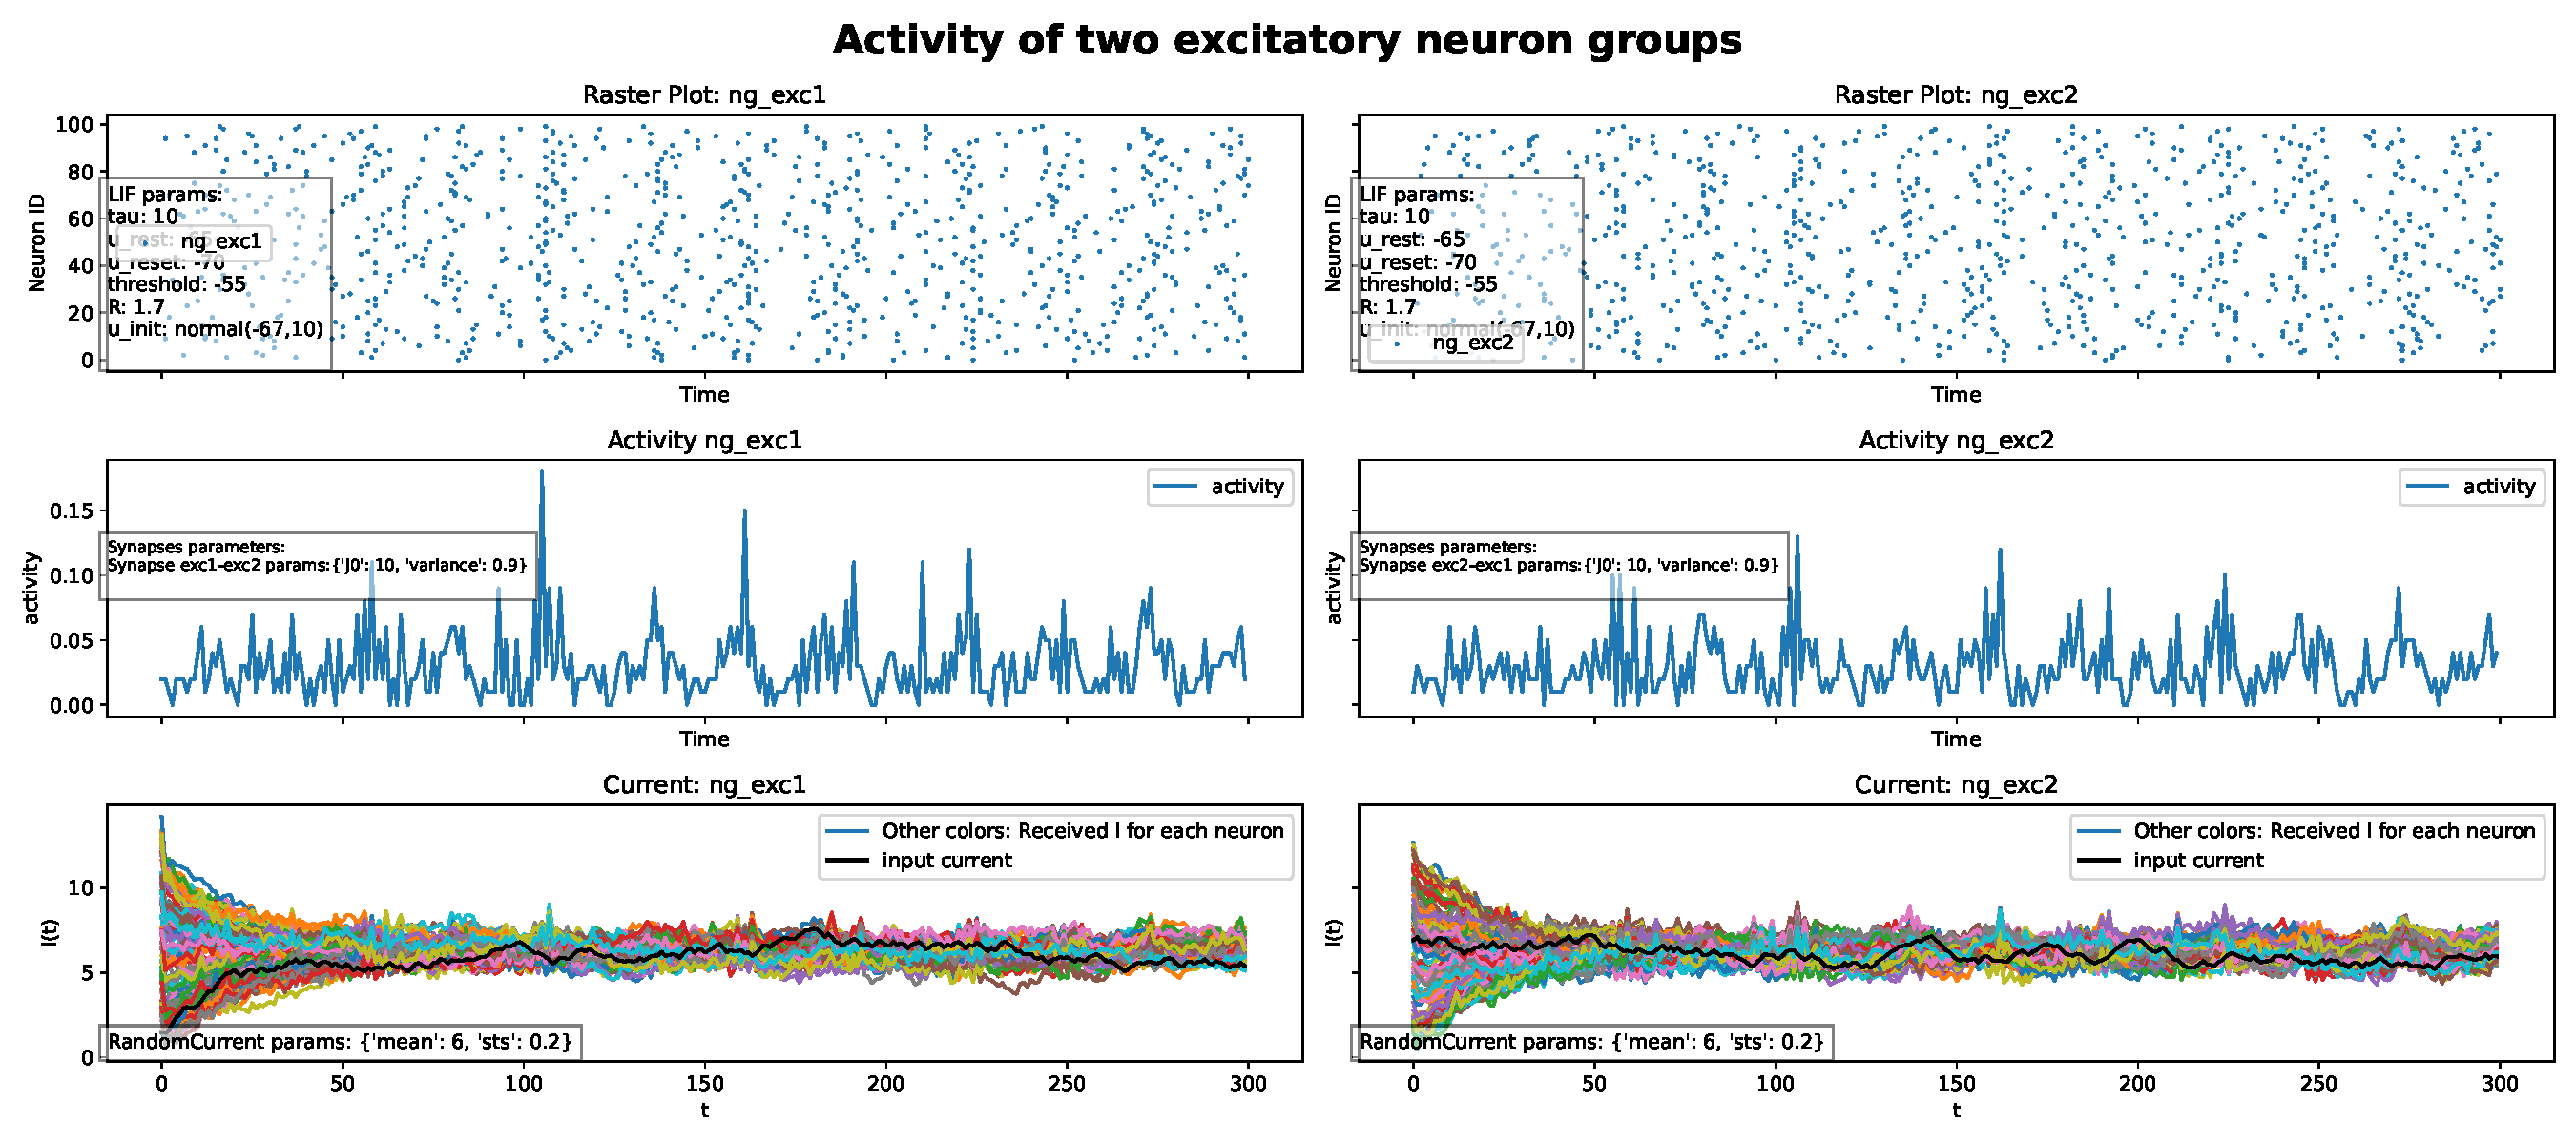
\includegraphics[width=0.9\textwidth]{plots/part2-two-ng-full-synapse-diff-variance-rand-curr.pdf} 
                \caption{رفتار دو جمعیت نورونی با دو سیناپس و جریان نویزی و واریانس متفاوت}
                \label{fig:part2-two-ng-full-synapse-diff-variance-rand-curr}
            \end{figure}
            همانطور که پیشتر گفته شد، اگر بخواهیم واریانس را به گونه ای تغییر دهیم که تاثیر قابل نمایشی داشته باشد، باید مقدار آن را زیادتر، مثلا ۱۰۰ بگیریم. مطابق شکل 
            \ref{fig:part2-two-ng-full-synapse-very-high-variance-noise-curr}
            تاثیر این مقدار نمایان است. این به این دلیل است که با خیلی زیاد شدن واریانس، بسیاری از وزن ها نیز آنقدر زیاد می شوند که تاثیر مجموع آن ها روی نورون های پس سیناپسی مشهود می شود.
            \begin{figure}[!ht]
                \centering
                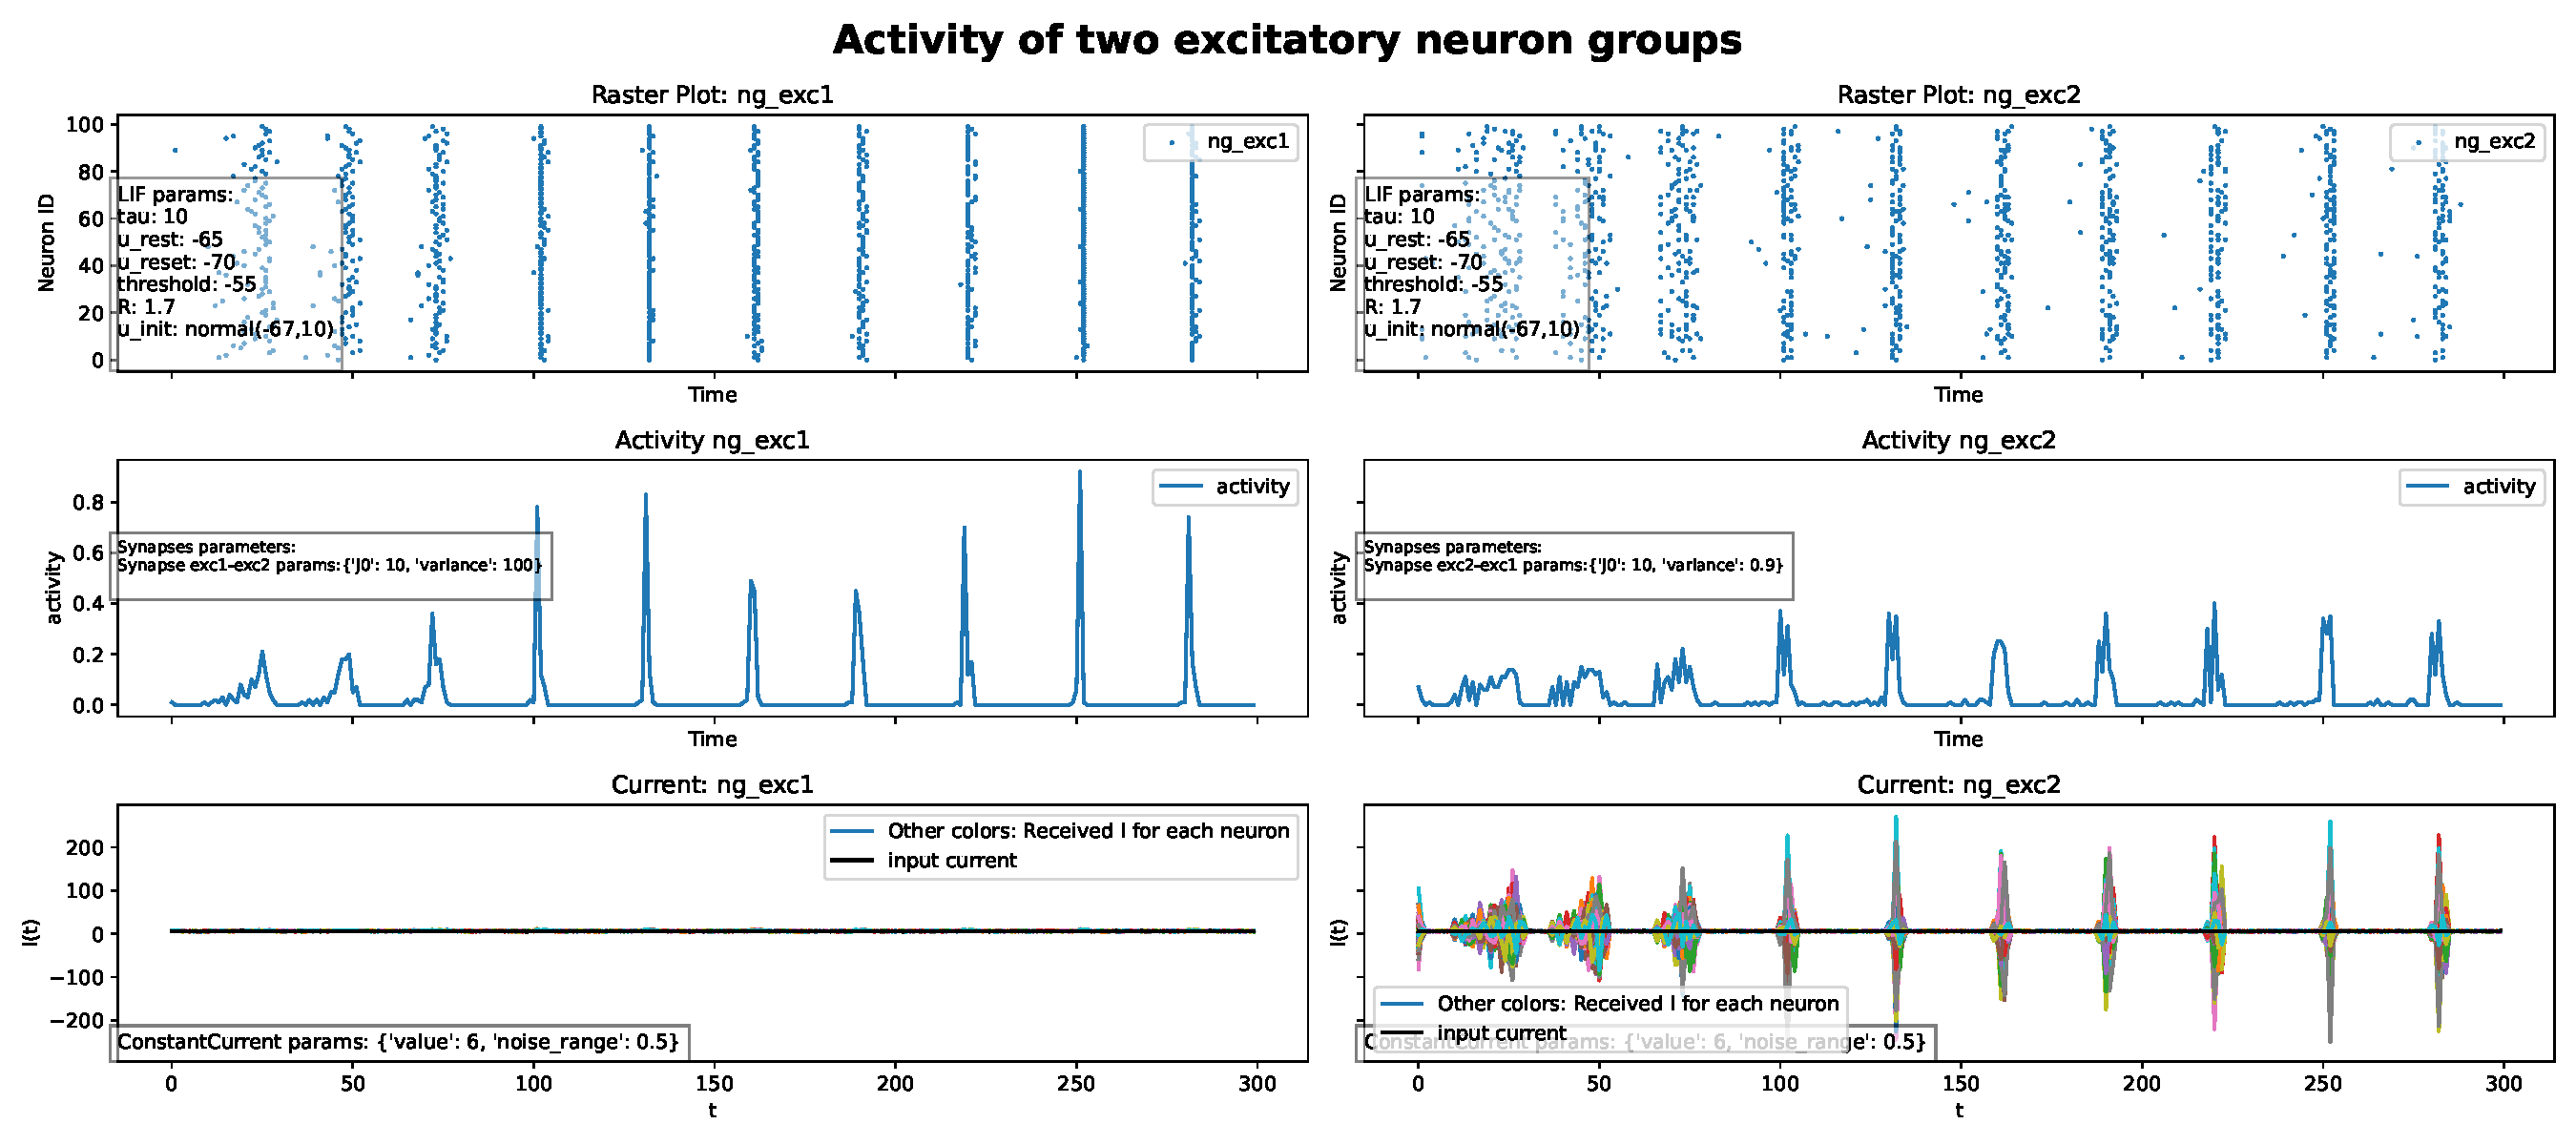
\includegraphics[width=0.9\textwidth]{plots/part2-two-ng-full-synapse-very-high-variance-noise-curr.pdf} 
                \caption{رفتار دو جمعیت نورونی با دو سیناپس و جریان نویزی و واریانس بسیار زیاد}
                \label{fig:part2-two-ng-full-synapse-very-high-variance-noise-curr}
            \end{figure}
            
            \paragraph*{تاثیر اندازه جمعیت}
            از آنجا که تنها دو جمعیت نورونی داریم، زیاد کردن هر دو جمعیت تاثیری مشابه تک جمعیت خواهد داشت، در نتیجه فقط حالتی را که یک جمعیت بزرگتر از دیگری است را آزمایش میکنیم. در این حالت نیز مشابه حالت های قبل میبینیم که فعالیت هر دو جمعیت پس از مدتی بیشتر می شود. هر چند میزان رشد جمعیت بزرگتر اندکی از جمعیت کوچکتر بیشتر است.
            (شکل \ref{fig:part2-two-ng-full-synapse-diff-size-noise-curr})
            \begin{figure}[!ht]
                \centering
                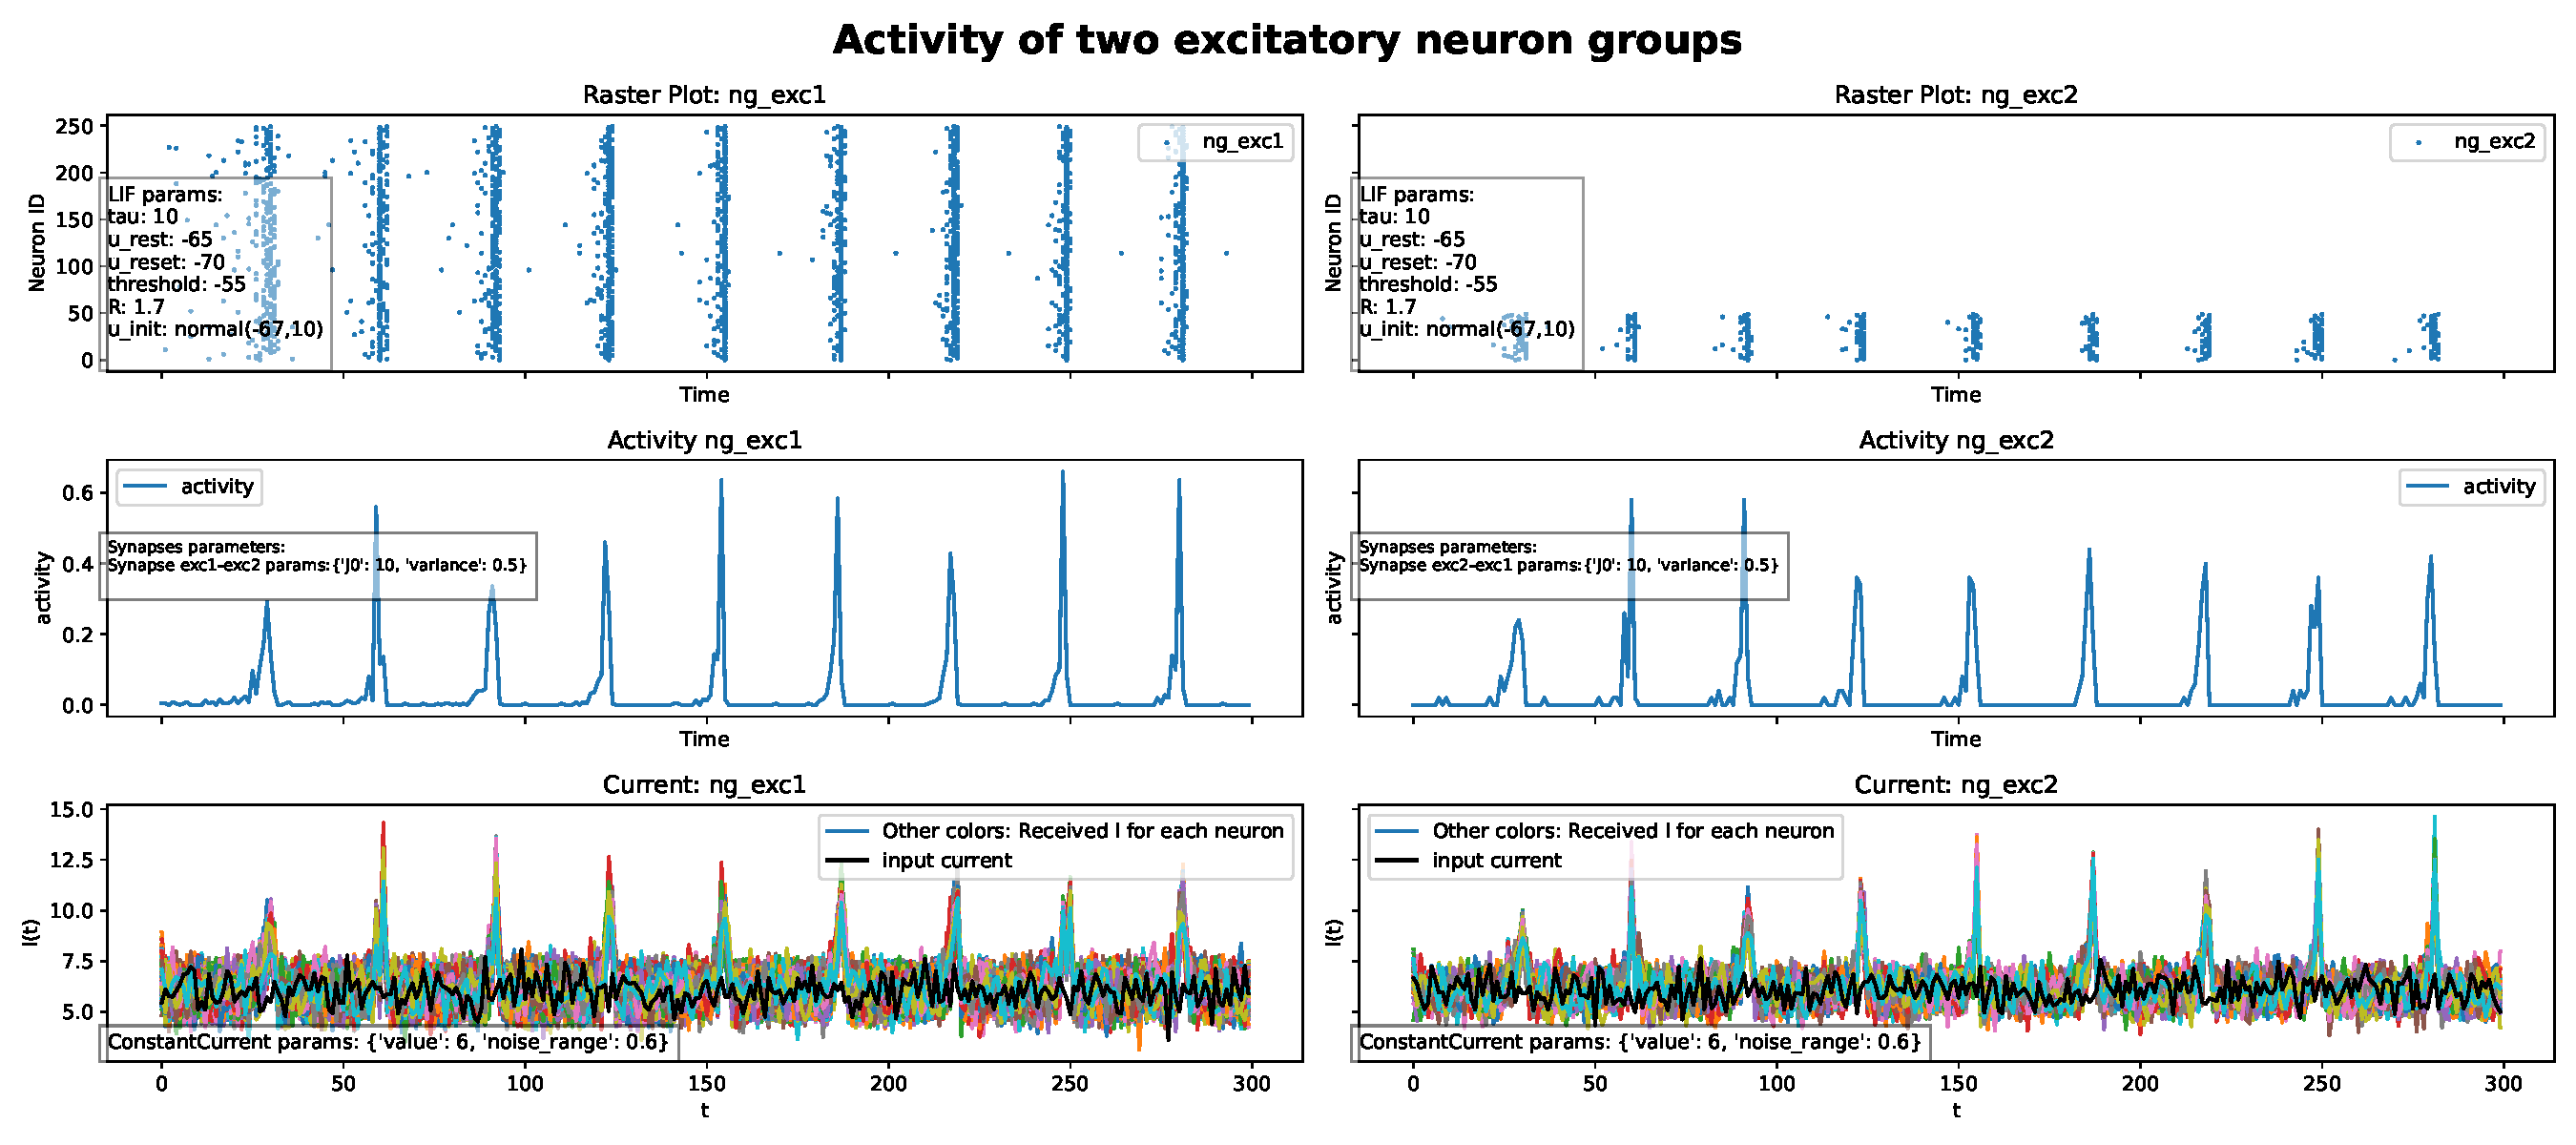
\includegraphics[width=0.9\textwidth]{plots/part2-two-ng-full-synapse-diff-size-noise-curr.pdf} 
                \caption{رفتار دو جمعیت نورونی با دو سیناپس و جریان نویزی و واریانس بسیار زیاد}
                \label{fig:part2-two-ng-full-synapse-diff-size-noise-curr}
            \end{figure}


    \subsection{الگوی ارتباط تصادفی با احتمال جفت شدن ثابت}
        در این قسمت به بررسی رفتار الگوی ارتباط تصادفی با احتمال جفت شدن ثابت می پردازیم. 

        از نظر تجربی، احتمال 
        $p$
        که یک نورون در داخل یک ستون قشر مغز، یک اتصال عملکردی به نورون دیگری در همان ستون برقرار کند، در محدوده 10 درصد است، هرچند این مقدار در بین لایه‌ها متفاوت است.

        در شبیه‌سازی‌ها، می‌توانیم یک احتمال اتصال 
        $p$ 
        را رفع کنیم و اتصالات را به‌طور تصادفی با احتمال 
        $p$ 
        از بین تمام اتصالات 
        $N^2$ 
        ممکن انتخاب کنیم. در این مورد، تعداد اتصال های ورودی پیش سیناپسی 
        $C_j$
        به یک نورون پس سیناپسی 
        $j$
        دارای مقدار میانگین 
        $\langle C_j = pN$
        است، اما بین یک نورون و نورون بعدی با واریانس 
        $p(1-p)N$ 
        در نوسان است.

        تا اینجای کار تاثیر بسیاری از پارامتر هایی که بررسی کردم شبیه تاثیر پارامتر های مشابه این الگو است. از این رو در این بخش تمرکزمان را روی پارامتر هایی میگذاریم که تاثیر متفاوت تری نسبت به حالت قبل دارند. در اینجا نیز مدل نورونی را مانند مدل های قبل درنظر میگیریم.
        \subsubsection*{بررسی رفتار یک جمعیت}
            برای شروع کار، بیایید رفتار یک جمعیت را با جریان ثابت بررسی کنیم. همانطور که از شکل 
            \ref{fig:part2-one-ng-prob-synapse-const-curr}
            بر می‌آید، رفتار نورون همانند الگوی ارتباط قبلی بوده و پس از مدتی، پراکندگی زمان ضربه زدن نورون ها کمتر شده و فعالیت رفته رفته بیشتر می شود. دلیل این امر نیز مشابه الگو های قبل، زیاد شدن جریان سیناپسی است.
            \begin{figure}[!ht]
                \centering
                \includegraphics[width=0.9\textwidth]{plots/part2-one-ng-prob-synapse-const-curr.pdf} 
                \caption{رفتار دو جمعیت نورونی با دو سیناپس و جریان نویزی و واریانس بسیار زیاد}
                \label{fig:part2-one-ng-prob-synapse-const-curr}
            \end{figure}
%%%%%%%%%%%%%%%%%%%%%%%%%%% Bibliography section %%%%%%%%%%%%%%%%%%%%%%%%%%%
\newpage
\begin{thebibliography}{1}
    \bibitem{textbook}
        \begin{latin}
            Computational Neuroscience Course, School of computer science, University of Tehran
        \end{latin}
    \bibitem{PymoNNtorch}
        \begin{latin}
            PymoNNtorchPytorch-adapted version of PymoNNto
        \end{latin}
    \bibitem{wikipedia-refractory-period}
        \begin{latin}
            \href{https://en.wikipedia.org/wiki/Refractory_period_(physiology)}{Wiki-pedia: Refractory\_period\_(physiology)}
        \end{latin}
    \bibitem{Neuronal-Dynamics}
        \begin{latin}
            \href{https://neuronaldynamics.epfl.ch/online/Ch12.S3.html}{Neuronal Dynamics, Wulfram Gerstner, Werner M. Kistler, Richard Naud and Liam Paninski
            }
        \end{latin}
    \end{thebibliography}
\end{document}
